\documentclass[10pt,twoside]{article}


\usepackage{iftex}

\ifPDFTeX
\usepackage[utf8]{inputenc}
\usepackage[T5]{fontenc}
\usepackage[vietnamese]{babel}
\usepackage{mathptmx}
\usepackage[scaled=0.92]{helvet}
\newcommand{\arialfont}{\fontfamily{phv}\selectfont}
\else
\usepackage[vietnamese]{babel}
\usepackage{fontspec}
\defaultfontfeatures{Ligatures=TeX}

\IfFontExistsTF{Times New Roman}
{\setmainfont{Times New Roman}}
{\setmainfont{TeX Gyre Termes}}

\IfFontExistsTF{Arial}
{\setsansfont{Arial}\newfontfamily\arialfont{Arial}}
{\setsansfont{TeX Gyre Heros}\newfontfamily\arialfont{TeX Gyre Heros}}
\fi

% ------------------ Page layout theo template FAIR ------------------
\usepackage[
paperwidth=20.5cm,
paperheight=29.5cm,
top=2.2cm,
bottom=1.8cm,
left=1.8cm,
right=1.8cm,
headheight=23pt,
headsep=0.55cm,
footskip=1cm
]{geometry}

% ------------------ Packages ------------------
\usepackage{amsmath,amssymb}
\usepackage{graphicx}
\usepackage{array}
\usepackage{booktabs}
\usepackage{caption}
\usepackage{subcaption}
\usepackage{float}
\usepackage{enumitem}
\usepackage{fancyhdr}
\usepackage{titlesec}
\usepackage{indentfirst}
\usepackage{etoolbox}
\usepackage{url}

% ------------------ Paragraph style ------------------
\setlength{\parindent}{1cm}
\setlength{\parskip}{6pt}
\linespread{1.0}
\emergencystretch=2em
\flushbottom

% ------------------ Float placement ------------------
% Cho phép LaTeX phân bố hình và bảng linh hoạt để tránh khoảng trắng lớn,
% nhưng vẫn giữ nguyên lề, cỡ chữ và khoảng cách đoạn của template.
\setcounter{topnumber}{5}
\setcounter{bottomnumber}{5}
\setcounter{totalnumber}{10}
\renewcommand{\topfraction}{0.95}
\renewcommand{\bottomfraction}{0.90}
\renewcommand{\textfraction}{0.05}
\renewcommand{\floatpagefraction}{0.80}

% ------------------ Paper metadata ------------------
\newcommand{\PaperTitle}{XẾP HẠNG TÍN DỤNG DOANH NGHIỆP DỰA TRÊN MÔ HÌNH HỌC MÁY}
\newcommand{\PaperShortTitle}{XẾP HẠNG TÍN DỤNG DOANH NGHIỆP DỰA TRÊN MÔ HÌNH HỌC MÁY}
\newcommand{\PaperAuthors}{Lê Nguyễn Thành Tài\textsuperscript{1}}
\newcommand{\PaperShortAuthors}{Lê Nguyễn Thành Tài}
\newcommand{\PaperAffiliations}{%
\textsuperscript{1}Khoa Công nghệ Thông tin, Trường Đại học Sư phạm kỹ thuật Vĩnh Long
}
\newcommand{\PaperEmail}{22022001@st.vlute.edu.vn}
\newcommand{\FairConference}{}

% ------------------ Header/Footer ------------------
\pagestyle{fancy}
\fancyhf{}

% Trang chẵn: số trang bên trái, tên bài bên phải.
% Trang lẻ: tác giả bên trái, số trang bên phải.
\fancyhead[LE]{\fontsize{9pt}{11pt}\selectfont\thepage}
\fancyhead[RE]{\fontsize{9pt}{11pt}\selectfont\PaperShortTitle}
\fancyhead[LO]{\fontsize{9pt}{11pt}\selectfont\PaperShortAuthors}
\fancyhead[RO]{\fontsize{9pt}{11pt}\selectfont\thepage}

% Template có đường kẻ mảnh dưới header ở các trang sau.
\renewcommand{\headrulewidth}{0.4pt}
\renewcommand{\footrulewidth}{0pt}

\fancypagestyle{firstpage}{%
\fancyhf{}%
\fancyhead[C]{\fontsize{9pt}{11pt}\selectfont\FairConference}%
\renewcommand{\headrulewidth}{0.4pt}
\renewcommand{\footrulewidth}{0pt}%
}

% ------------------ Title block ------------------
\newcommand{\makefairtitle}{%
\thispagestyle{firstpage}%
\begin{center}
{\arialfont\bfseries\fontsize{14pt}{16pt}\selectfont\MakeUppercase{\PaperTitle}\par}
\vspace{3pt}
{\bfseries\normalsize\PaperAuthors\par}
\vspace{3pt}
{\fontsize{9pt}{11pt}\selectfont\PaperAffiliations\par}
\vspace{3pt}
{\itshape\fontsize{9pt}{11pt}\selectfont\PaperEmail\par}
\end{center}
\vspace{6pt}%
}

% ------------------ Abstract / Keywords ------------------
\newcommand{\FairDash}{\unskip\textemdash\space}

\newenvironment{fairabstract}{%
\begingroup
\fontsize{9pt}{11pt}\selectfont
\itshape
\setlength{\parindent}{1cm}%
\setlength{\parskip}{6pt}%
}{%
\par\endgroup
}

\newcommand{\fairabstracttext}[1]{%
\begin{fairabstract}
\textbf{TÓM TẮT}\FairDash #1
\end{fairabstract}
}

\newcommand{\fairkeywords}[1]{%
\begin{fairabstract}
\textbf{Từ khóa}\FairDash #1
\end{fairabstract}
}

% ------------------ Section numbering ------------------
\setcounter{secnumdepth}{4}

\renewcommand{\thesection}{\Roman{section}}
\renewcommand{\thesubsection}{\Alph{subsection}}
\renewcommand{\thesubsubsection}{\arabic{subsubsection}}
\renewcommand{\theparagraph}{\alph{paragraph}}

\titleformat{\section}
{\centering\normalsize\bfseries}
{\thesection.}{0.5em}{}

\titleformat{\subsection}
{\normalsize\bfseries\itshape}
{\thesubsection.}{0.5em}{}

\titleformat{\subsubsection}
{\normalsize\bfseries\itshape}
{\thesubsubsection.}{0.5em}{}

\titleformat{\paragraph}[block]
{\normalsize}
{\theparagraph)}{0.5em}{}

\titlespacing*{\section}{0pt}{6pt}{6pt}
\titlespacing*{\subsection}{0pt}{6pt}{3pt}
\titlespacing*{\subsubsection}{0pt}{6pt}{3pt}
\titlespacing*{\paragraph}{0pt}{6pt}{3pt}

% ------------------ Figure/Table captions ------------------
\renewcommand{\figurename}{Hình}
\renewcommand{\tablename}{Bảng}

\captionsetup{
font=small,
labelsep=period,
justification=centering,
singlelinecheck=true,
skip=3pt
}


% ------------------ Lists ------------------
\setlist[itemize]{
leftmargin=1.27cm,
itemsep=0pt,
topsep=0pt,
parsep=0pt
}

\setlist[enumerate]{
leftmargin=1.27cm,
itemsep=0pt,
topsep=0pt,
parsep=0pt
}

% ------------------ Bibliography ------------------
% Giữ tiêu đề TÀI LIỆU THAM KHẢO theo kiểu section nhưng không đánh số.
\makeatletter
\renewenvironment{thebibliography}[1]{%
\section*{TÀI LIỆU THAM KHẢO}%
\fontsize{9pt}{11pt}\selectfont
\hbadness=10000
\setlength{\parskip}{0pt}%
\list{[\arabic{enumiv}]}{%
\settowidth\labelwidth{[#1]}%
\leftmargin\labelwidth
\advance\leftmargin\labelsep
\usecounter{enumiv}%
\let\p@enumiv\@empty
\renewcommand{\theenumiv}{\arabic{enumiv}}%
}%
\sloppy
\clubpenalty4000
\widowpenalty4000
}{%
\endlist
}
\makeatother

\urlstyle{same}

% =========================================================
% DOCUMENT
% =========================================================
\begin{document}

\makefairtitle

\fairabstracttext{%
Xếp hạng tín dụng doanh nghiệp hỗ trợ đánh giá sức khỏe tài chính, khả năng thực hiện nghĩa vụ nợ và cảnh báo sớm rủi ro. Nghiên cứu này xây dựng một hệ thống xếp hạng tín dụng dựa trên dữ liệu tài chính và so sánh các mô hình LightGBM, XGBoost, LSTM, TCN, PatchTST, Transformer-LSTM và GraphSAGE. Tập dữ liệu thực nghiệm gồm 8.680 quan sát của 1.623 doanh nghiệp trong giai đoạn 2005--2016. Mỗi quan sát được biểu diễn bằng 12 chỉ số thuộc các nhóm thanh khoản, đòn bẩy, sinh lời, hiệu quả hoạt động và dòng tiền, đồng thời được phân loại thành ba nhóm Distressed, High Yield và Investment Grade. Bên cạnh các mô hình riêng lẻ, nghiên cứu triển khai Fuzzy Choquet Integral, Gompertz Fuzzy Ranking và đề xuất Dynamic Model Fusion kết hợp Transformer-LSTM với GraphSAGE. Khi hai mô hình thành phần đưa ra dự báo khác nhau, cơ chế Dynamic Classifier Selection lựa chọn mô hình dựa trên năng lực trên tập xác thực và độ tin cậy đối với từng mẫu. Dynamic Model Fusion đạt kết quả tổng thể cao nhất trên tập kiểm thử, với Accuracy 92,98\%, Precision 92,67\%, Recall 92,98\% và F1-score 92,60\%. GradientSHAP và LIME được sử dụng để phân tích ảnh hưởng của các đặc trưng tài chính. Kết quả giải thích ghi nhận vai trò đáng kể của biên lợi nhuận, tỷ lệ nợ trên vốn chủ sở hữu và khả năng thanh khoản, qua đó hỗ trợ diễn giải quyết định phân loại của hệ thống.
}

\fairkeywords{%
Xếp hạng tín dụng doanh nghiệp, Học máy, Học sâu, Học tập hợp, Trí tuệ nhân tạo có khả năng giải thích.
}

\section{GIỚI THIỆU}
\subsection{Giới thiệu bài toán}
Xếp hạng tín dụng doanh nghiệp phản ánh khả năng thanh toán, mức độ rủi ro và sức khỏe tài chính của doanh nghiệp. Trong bối cảnh lãi suất và thị trường vốn biến động, việc đánh giá rủi ro vỡ nợ có ý nghĩa đối với ngân hàng, nhà đầu tư và cơ quan quản lý.

Theo S\&P Global Ratings, năm 2025 ghi nhận 117 vụ vỡ nợ trên toàn cầu, với tổng giá trị nợ mất khả năng thanh toán vượt 140 tỷ USD \cite{noauthor_default_nodate}. Quy mô thị trường trái phiếu bằng đồng nội tệ tại Đông Á mới nổi đạt khoảng 29,5 nghìn tỷ USD vào cuối năm 2025 \cite{bank_asia_2025}. Tại Việt Nam, quy mô thị trường trái phiếu doanh nghiệp đạt khoảng 1,42 triệu tỷ đồng, tương đương gần 11\% GDP; lượng phát hành mới trong năm 2025 tăng 32\% và vượt 624 nghìn tỷ đồng \cite{noauthor_tong_nodate}. Các số liệu này cho thấy nhu cầu đối với phương pháp đánh giá tín dụng có khả năng kiểm chứng và diễn giải.

Dữ liệu tài chính thường biến động, trong khi quan hệ giữa các chỉ số tài chính và rủi ro tín dụng có thể phi tuyến. Phương pháp đánh giá truyền thống phụ thuộc vào chuyên gia; ngược lại, các mô hình học máy có thể khó diễn giải khi được sử dụng như hệ thống ``hộp đen''. Nghiên cứu này vì vậy xây dựng và so sánh các mô hình học máy, học sâu và mô hình đồ thị cho phân loại rủi ro tín dụng, đồng thời sử dụng XAI để phân tích vai trò của các chỉ số tài chính trong dự báo.
\subsection{Bối cảnh và khoảng trống nghiên cứu}
Các nghiên cứu về dữ liệu doanh nghiệp dạng bảng cho thấy các mô hình cây tăng cường vẫn là đường cơ sở cạnh tranh. Trương Thị Thùy Dương và Lê Hải Trung \cite{thuy_ung_2023} đánh giá sáu thuật toán trên 300 doanh nghiệp Việt Nam giai đoạn 2017--2019; XGBoost đạt Accuracy 87,73\%, cao hơn Random Forest với 83,49\%. Trên bộ dữ liệu lớn hơn, Andersson \cite{andersson_masters_nodate} ghi nhận Gradient Boosting đạt Accuracy xấp xỉ 90\% khi dự báo xếp hạng của Standard \& Poor's, Moody's và Fitch.

Các kiến trúc học sâu mở rộng khả năng khai thác phụ thuộc theo thời gian và thông tin đa phương thức. Kofune và cộng sự \cite{kofune_enhancing_2026} đề xuất Transformer-LSTM và đạt Accuracy 89,96\%. Chen và Long \cite{chen_novel_2020} sử dụng Self-Attention trong mô hình SMAGRU, với Accuracy 93,33\%. Morthens \cite{morthens_credit_nodate} kết hợp mô hình tuần tự và mô hình đồ thị để khai thác dữ liệu tài chính theo thời gian cùng quan hệ doanh nghiệp; GRU và GRU-GCNGRU lần lượt đạt 75,25\% và 74,44\%. Fang và cộng sự \cite{fang_design_2025} kết hợp chọn lọc đặc trưng, lấy mẫu tăng cường và CNN-BiLSTM-AM trên dữ liệu văn bản tài chính, đạt Accuracy 88\%.

Đối với hướng tiếp cận đồ thị, Feng và cộng sự \cite{feng_every_2020} đề xuất CCR-GNN cho xếp hạng tín dụng doanh nghiệp và báo cáo Accuracy 95\% trên dữ liệu doanh nghiệp niêm yết tại Trung Quốc. Công trình tiếp theo phát triển HHGNN để khai thác cấu trúc phân cấp, tính không đồng nhất và dữ liệu chưa gán nhãn trong mạng lưới doanh nghiệp, đạt Accuracy 97,557\% \cite{feng_corporate_2024}. Liu và Kok \cite{liu_prediction_2025} sử dụng Heterogeneous Topological Graph Neural Network cho dự báo xếp hạng tín dụng ngân hàng và đạt Accuracy 70,57\%. Các kết quả này cho thấy hiệu quả của từng kiến trúc phụ thuộc đáng kể vào nguồn dữ liệu và giao thức đánh giá. Nghiên cứu hiện tại vì vậy đánh giá thống nhất các mô hình cây, mô hình chuỗi và mô hình đồ thị trên cùng một tập dữ liệu, đồng thời khảo sát cơ chế kết hợp động và khả năng giải thích dự báo.
\section{CÁC CÔNG VIỆC LIÊN QUAN}

\subsection{Đặc điểm của Xếp hạng tín dụng doanh nghiệp}

Xếp hạng tín dụng doanh nghiệp đánh giá mức độ tin cậy tài chính và khả năng thực hiện nghĩa vụ nợ trong một khoảng thời gian xác định \cite{phu_nghi_nodate}. Kết quả xếp hạng hỗ trợ ngân hàng, nhà đầu tư và cơ quan quản lý trong cấp tín dụng, đầu tư trái phiếu và giám sát rủi ro \cite{hai_mo_2023}. Doanh nghiệp có khả năng sinh lời, dòng tiền ổn định và đòn bẩy thấp thường thuộc nhóm tín dụng tốt hơn; doanh nghiệp có dòng tiền yếu, nợ vay lớn hoặc nguy cơ mất khả năng thanh toán thuộc nhóm rủi ro cao hơn \cite{thuy_ung_2023}.

Nghiên cứu phân chia xếp hạng thành ba nhóm: Investment Grade (IG), High Yield (HY) và Distressed. IG biểu thị mức rủi ro thấp; HY có mức rủi ro cao hơn; Distressed đại diện cho tình trạng tài chính yếu và nguy cơ vỡ nợ lớn \cite{hung_xep_2023}. Mối quan hệ giữa các chỉ số thanh khoản, đòn bẩy, sinh lời và dòng tiền với rủi ro tín dụng thường phi tuyến và thay đổi theo thời gian \cite{hai_mo_2023}. Vì vậy, nghiên cứu kết hợp học máy, học sâu và trí tuệ nhân tạo có khả năng giải thích (Explainable AI, XAI) để đánh giá hiệu quả phân loại và hỗ trợ diễn giải vai trò của các chỉ số tài chính \cite{gramegna_shap_2021}.
\subsection{Các mô hình học máy và học sâu}

\subsubsection{Mô hình LightGBM (Light Gradient Boosting Machine)}
LightGBM (Light Gradient Boosting Machine) là thuật toán học tập hợp thuộc họ cây quyết định tăng cường theo gradient (GBDT) \cite{ke_lightgbm_2017}. Thuật toán sử dụng chiến lược phát triển cây theo lá và các kỹ thuật lấy mẫu, gom đặc trưng để giảm chi phí tính toán và bộ nhớ trên dữ liệu nhiều chiều.
\subsubsection{Mô hình XGBoost (eXtreme Gradient Boosting)}
XGBoost (eXtreme Gradient Boosting) là một triển khai GBDT có khả năng mở rộng, kết hợp hàm mục tiêu chính quy hóa và các kỹ thuật tối ưu tính toán \cite{chen_xgboost_2016}. Cơ chế này hỗ trợ kiểm soát độ phức tạp của mô hình và xử lý hiệu quả dữ liệu dạng bảng.
\subsubsection{Mạng tích chập thời gian (Temporal Convolutional Network - TCN)}
Mạng tích chập thời gian (Temporal Convolutional Network, TCN) sử dụng tích chập nhân quả và tích chập giãn để xử lý dữ liệu tuần tự \cite{bai_empirical_2018}. So với kiến trúc hồi tiếp, TCN cho phép tính toán song song và mở rộng trường tiếp nhận mà không làm vi phạm thứ tự thời gian.
\subsubsection{Mạng nơ-ron bộ nhớ ngắn hạn dài (Long Short-Term Memory - LSTM)}
Mạng bộ nhớ dài-ngắn hạn (Long Short-Term Memory, LSTM) là một biến thể của mạng nơ-ron hồi tiếp, sử dụng trạng thái bộ nhớ và các cổng điều khiển để giảm ảnh hưởng của hiện tượng tiêu biến gradient \cite{hochreiter_long_1997}. Nhờ đó, LSTM có thể học phụ thuộc dài hạn trong chuỗi dữ liệu.
\subsubsection{Kiến trúc PatchTST (Patch Time Series Transformer)}
PatchTST chia chuỗi thời gian thành các đoạn con (patch) và sử dụng Transformer để học biểu diễn giữa các đoạn \cite{nie_time_2023}. Cách biểu diễn này giảm độ dài chuỗi đầu vào và hỗ trợ mô hình khai thác đồng thời cấu trúc cục bộ và phụ thuộc dài hạn.
\subsubsection{Mô hình lai T-LSTM (Transformer-Long Short-Term Memory)}
Mô hình lai T-LSTM (Transformer-Long Short-Term Memory) \cite{kofune_enhancing_2026} là kiến trúc kết hợp giữa Transformer và LSTM nhằm khai thác hiệu quả dữ liệu tài chính dạng chuỗi thời gian. Trong bài toán xếp hạng tín dụng doanh nghiệp, dữ liệu tài chính không chỉ phản ánh trạng thái tại một thời điểm mà còn thể hiện xu hướng biến động của doanh nghiệp qua nhiều kỳ liên tiếp. Vì vậy, mô hình T-LSTM được sử dụng để học đồng thời các quan hệ dài hạn và sự phụ thuộc tuần tự trong chuỗi chỉ số tài chính.
\subsubsection{Mạng nơ ron đồ thị GraphSAGE (Graph Sample and Aggregate)}
GraphSAGE là một khung học biểu diễn nút theo hướng quy nạp, trong đó biểu diễn của mỗi nút được hình thành bằng cách tổng hợp đặc trưng của nút và các nút lân cận \cite{hamilton_inductive_2018}. Khác với phương pháp học một vector cố định cho từng nút, GraphSAGE có thể tạo biểu diễn cho các nút chưa xuất hiện trong quá trình huấn luyện.
\subsubsection{Độ đo đánh giá mô hình} 
\paragraph{Accuracy} 
Accuracy \cite{grandini_metrics_2020} hay độ chính xác, là tỷ lệ giữa số mẫu được mô hình dự đoán đúng trên tổng số mẫu trong tập dữ liệu. Đây là một độ đo đơn giản, dễ hiểu và thường được sử dụng trong các bài toán phân loại để đánh giá hiệu suất tổng quát của mô hình. Công thức tính Accuracy được biểu diễn như sau: 
\begin{equation} Accuracy = \frac{TP + TN}{TP + TN + FP + FN} 
\end{equation} Trong đó: 
\begin{itemize} 
\item $TP$ (True Positive): số lượng mẫu dương tính được dự đoán đúng. 
\item $TN$ (True Negative): số lượng mẫu âm tính được dự đoán đúng. 
\item $FP$ (False Positive): số lượng mẫu âm tính nhưng bị dự đoán nhầm là dương tính. 
\item $FN$ (False Negative): số lượng mẫu dương tính nhưng bị dự đoán nhầm là âm tính. 
\end{itemize}
\paragraph{Precision} 
Precision \cite{grandini_metrics_2020} đo lường tỷ lệ dự đoán dương chính xác trên tổng số dự đoán dương. Điều này đặc biệt quan trọng trong các ứng dụng mà dự đoán dương giả (false positives) có thể gây hậu quả nghiêm trọng.
\begin{equation} 
\mathrm{Precision}=\frac{TP}{TP+FP}
\end{equation}
\paragraph{Recall} 
Recall \cite{grandini_metrics_2020} đo lường tỷ lệ dự đoán dương chính xác trên tổng số các mẫu thực tế là dương. Recall quan trọng trong các tình huống cần phát hiện tất cả các trường hợp dương, ngay cả khi điều đó dẫn đến việc dự đoán một số trường hợp âm là dương (false negatives).
\begin{equation} 
\mathrm{Recall}=\frac{TP}{TP+FN}
\end{equation}
\paragraph{F1-score} 
F1-score \cite{grandini_metrics_2020} là trung bình điều hòa của Precision và Recall. Chỉ số này cân bằng giữa độ chính xác của các dự đoán dương và khả năng phát hiện các mẫu dương.
\begin{equation} 
F1=2\times\frac{\mathrm{Precision}\times\mathrm{Recall}}{\mathrm{Precision}+\mathrm{Recall}}
\end{equation}
\paragraph{AUC-ROC} 
ROC Curve biểu diễn mối quan hệ giữa True Positive Rate (Recall) và False Positive Rate. AUC là diện tích dưới đường cong ROC và thể hiện khả năng phân biệt giữa các lớp của mô hình \cite{fawcett_introduction_2006}. Một mô hình với AUC gần 1 là một mô hình tốt, trong khi AUC gần 0.5 cho thấy mô hình hoạt động như ngẫu nhiên.
\begin{equation} 
\mathrm{TPR}=\frac{TP}{TP+FN}\quad;\quad \mathrm{FPR}=\frac{FP}{FP+TN}
\end{equation}

\subsection{Các phương pháp học kết hợp}
\subsubsection{Fuzzy Choquet Integral} Fuzzy Choquet Integral là phương pháp học kết hợp dựa trên độ đo mờ, được sử dụng để tổng hợp kết quả dự đoán từ nhiều mô hình thành phần. Khác với trung bình có trọng số, phương pháp này không chỉ xét mức độ quan trọng riêng lẻ của từng mô hình mà còn biểu diễn được quan hệ tương tác giữa các mô hình trong ensemble \cite{zadeh_fuzzy_1965, choquet_theory_1954}. Giả sử $x_1, x_2, \ldots, x_n$ là xác suất dự đoán của $n$ mô hình, được sắp xếp tăng dần $x_{(1)} \leq x_{(2)} \leq \cdots \leq x_{(n)}$. Tích phân Choquet rời rạc được tính như sau: \begin{equation} C_{\mu}(x) = \sum_{i=1}^{n} \left(x_{(i)} - x_{(i-1)}\right)\mu(A_{(i)}), \end{equation} trong đó $x_{(0)}=0$, $A_{(i)}=\{(i),(i+1),\ldots,(n)\}$ và $\mu(A_{(i)})$ là độ đo mờ biểu diễn mức độ quan trọng của tập các mô hình tương ứng.

\subsubsection{Gompertz Fuzzy Ranking} 
Gompertz Fuzzy Ranking là phương pháp học kết hợp sử dụng hàm Gompertz để gán trọng số mờ cho các mô hình dựa trên thứ hạng xác suất dự báo. Thay vì trung bình trực tiếp đầu ra của các mô hình, phương pháp này ưu tiên các mô hình có dự đoán tin cậy hơn và giảm ảnh hưởng của các mô hình có xác suất thấp \cite{kundu_fuzzy_2021}. Giả sử $p_i^{(c)}$ là xác suất dự báo của mô hình thứ $i$ đối với lớp $c$. Các xác suất được sắp xếp theo thứ hạng $r_i$, trong đó mô hình có xác suất cao hơn sẽ có thứ hạng tốt hơn. Trọng số mờ Gompertz được xác định như sau: 
\begin{equation} 
w_i = \frac{\exp \left(-\alpha e^{-\beta r_i}\right)} {\sum_{j=1}^{M} \exp \left(-\alpha e^{-\beta r_j}\right)} 
\end{equation} 
trong đó $M$ là số mô hình thành phần, $\alpha$ và $\beta$ là các tham số điều chỉnh độ dốc của hàm Gompertz. Điểm dự báo tổng hợp cho lớp $c$ được tính bởi: 
\begin{equation} 
S_c = \sum_{i=1}^{M} w_i p_i^{(c)} 
\end{equation} 
Nhãn dự đoán cuối cùng được xác định theo lớp có điểm tổng hợp lớn nhất. Trong nghiên cứu này, Gompertz Fuzzy Ranking được sử dụng để điều chỉnh đóng góp của các mô hình thành phần theo thứ hạng xác suất dự báo.
\subsubsection{Dynamic Model Fusion} Dynamic Model Fusion (DMF) là phương pháp kết hợp mô hình theo hướng động, trong đó kết quả cuối cùng được điều chỉnh theo mức độ tin cậy của từng mô hình đối với từng mẫu dữ liệu. Khác với các phương pháp voting hoặc averaging sử dụng trọng số cố định, DMF kết hợp với Dynamic Classifier Selection (DCS) để lựa chọn mô hình phù hợp hơn trong từng trường hợp \cite{toufiq_explainable_2026}. Trong nghiên cứu này, DMF được sử dụng để kết hợp hai mô hình T-LSTM và GraphSAGE. T-LSTM có ưu thế trong khai thác xu hướng tài chính theo thời gian, trong khi GraphSAGE hỗ trợ học quan hệ đồ thị giữa các doanh nghiệp. Gọi $\hat{y}_{T}$ và $\hat{y}_{G}$ lần lượt là nhãn dự đoán của T-LSTM và GraphSAGE. Nếu hai mô hình cho cùng một nhãn, kết quả cuối cùng được xác định như sau: 
\begin{equation} 
\hat{y} = \hat{y}_{T} = \hat{y}_{G} 
\end{equation} Ngược lại, nếu hai mô hình dự đoán khác nhau, hệ thống tính điểm tin cậy động cho từng mô hình dựa trên năng lực trên tập xác thực và xác suất dự đoán của mẫu kiểm thử: 
\begin{equation} 
R_m(x) = \lambda V_m(\hat{y}_m) + (1-\lambda) P_m(\hat{y}_m|x), 
\end{equation} trong đó $R_m(x)$ là điểm tin cậy của mô hình $m$, $V_m(\hat{y}_m)$ là năng lực của mô hình trên tập xác thực đối với lớp được dự đoán, $P_m(\hat{y}_m|x)$ là xác suất dự đoán của mô hình đối với mẫu $x$, và $\lambda$ là hệ số cân bằng. Nhãn cuối cùng được chọn từ mô hình có điểm tin cậy cao hơn: 
\begin{equation} 
\hat{y} = \hat{y}_{m^*}, \quad m^* = \arg\max_{m \in \{T,G\}} R_m(x). 
\end{equation} Cơ chế lựa chọn động cho phép DMF khai thác thông tin bổ sung từ mô hình chuỗi thời gian và mô hình đồ thị.
\subsection{Các phương pháp trí tuệ nhân tạo có khả năng giải thích}
\subsubsection{GradientSHAP} 
GradientSHAP là phương pháp giải thích dựa trên gradient, kết hợp ý tưởng của SHAP với cách lấy mẫu ngẫu nhiên giữa dữ liệu cần giải thích và các mẫu nền. Phương pháp này ước lượng mức đóng góp của từng đặc trưng bằng cách tính gradient của đầu ra mô hình theo đầu vào tại nhiều điểm nội suy giữa mẫu cần giải thích và các mẫu baseline \cite{lundberg_unified_2017, kokhlikyan_captum_2020}. 
\subsubsection{LIME} 
LIME là phương pháp giải thích cục bộ độc lập với mô hình, được Ribeiro và cộng sự đề xuất nhằm giải thích một dự báo cụ thể bằng một mô hình đơn giản tại vùng lân cận của mẫu cần phân tích \cite{ribeiro_why_2016}. Ý tưởng chính của LIME là tạo ra nhiều mẫu nhiễu xung quanh quan sát gốc, đưa các mẫu này vào mô hình để lấy xác suất dự báo, sau đó huấn luyện một mô hình tuyến tính cục bộ có trọng số để xấp xỉ hành vi của mô hình gốc.
\section{PHƯƠNG PHÁP ĐỀ XUẤT}
Nghiên cứu đề xuất một hệ thống gồm hai pha: huấn luyện và kiểm thử. Quy trình tổng thể được trình bày trong Hình~\ref{fig:proposed_model}.
\begin{figure}[!htbp]
    \centering % Căn giữa hình ảnh
    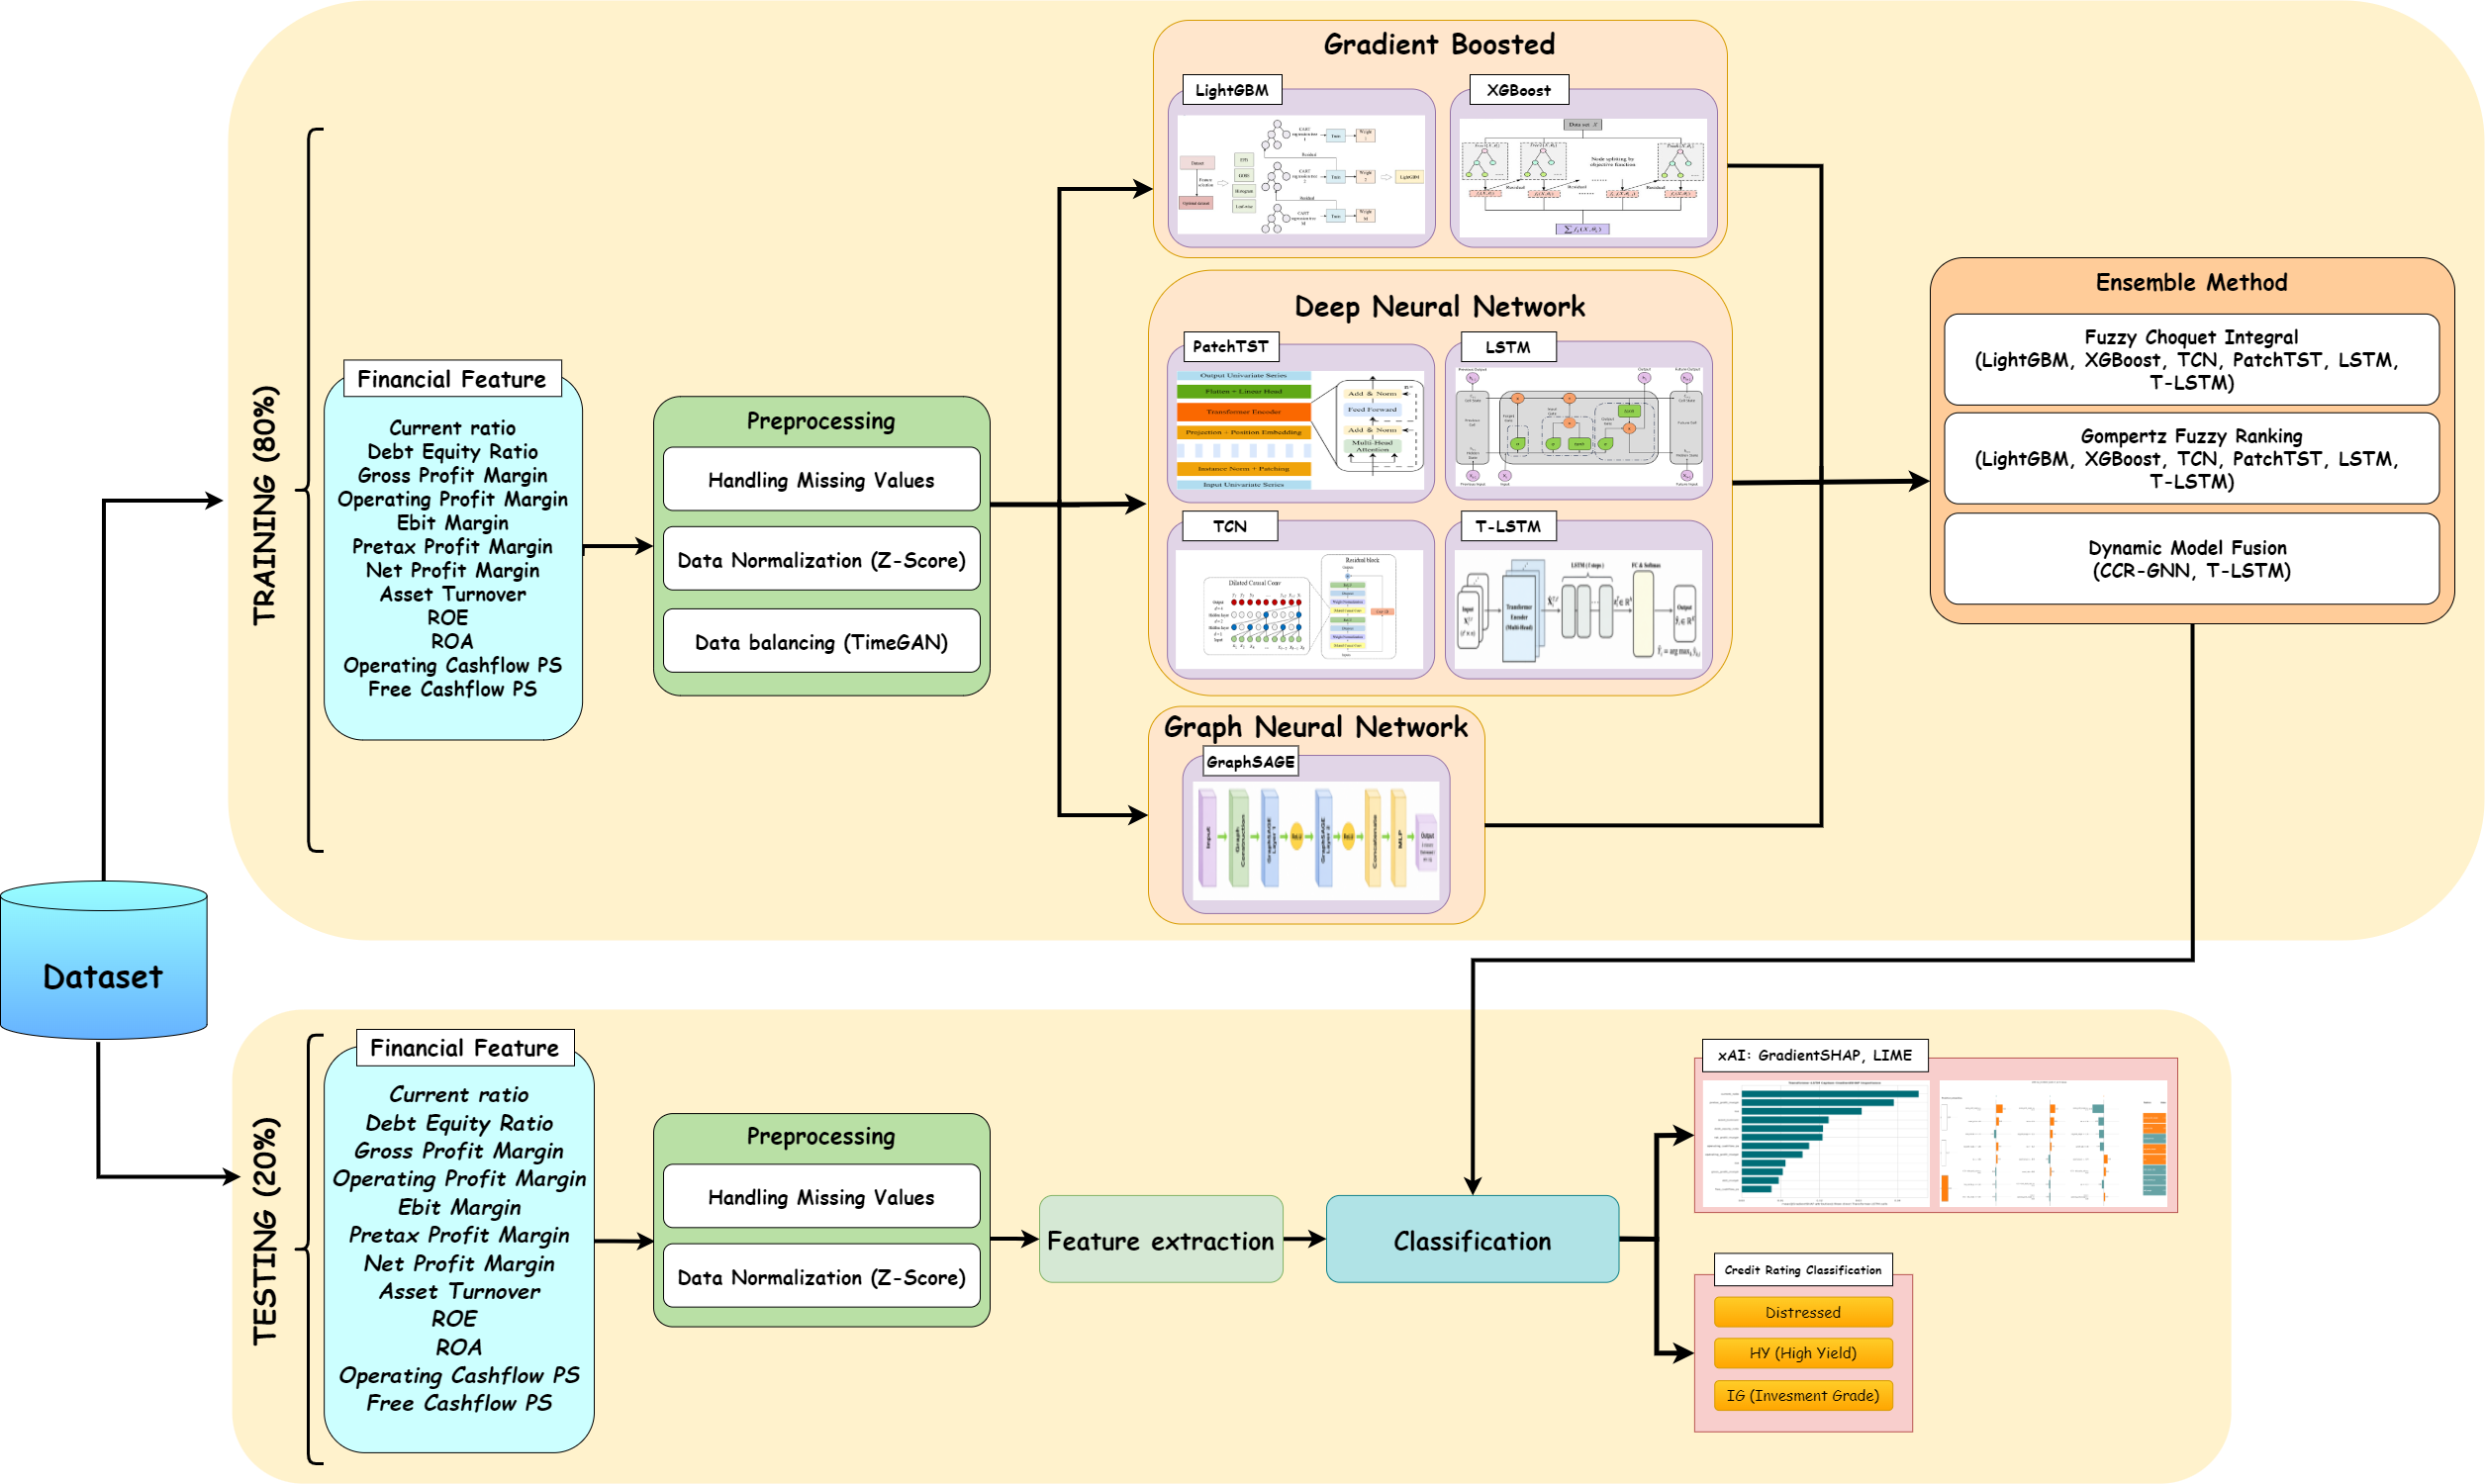
\includegraphics[width=1\textwidth]{uploads/sodo.drawio.drawio.png} % Thay 'ten-file-anh' bằng tên ảnh của bạn (không cần đuôi .png/.jpg)
    \caption{Mô hình đề xuất} % Dòng chú thích dưới ảnh
    \label{fig:proposed_model}
\end{figure}
\subsection{Pha huấn luyện} 
\subsubsection{Tiền xử lý dữ liệu và chuẩn bị dữ liệu} 
Trong pha huấn luyện, các bản ghi trùng lặp theo mã chứng khoán và ngày xếp hạng được gộp lại. Giá trị trung vị được sử dụng cho các chỉ số tài chính, còn nhãn xếp hạng được chọn theo mức rủi ro cao hơn để duy trì nguyên tắc thận trọng. Giá trị khuyết thiếu được điền bằng trung vị ước lượng từ tập huấn luyện nhằm hạn chế ảnh hưởng của ngoại lệ và tránh rò rỉ dữ liệu.

Các đặc trưng có phân phối lệch được biến đổi logarit khi độ lệch vượt ngưỡng xác định trước. Sau đó, 12 chỉ số tài chính được chuẩn hóa bằng Z-score để giảm ảnh hưởng của khác biệt về thang đo. Hai mươi mốt hạng tín dụng ban đầu được gộp thành ba nhóm Investment Grade (IG), High Yield (HY) và Distressed nhằm giảm độ thưa của nhãn trong khi vẫn duy trì thứ tự rủi ro.

Dữ liệu được sắp xếp theo doanh nghiệp và thời gian để tạo các cửa sổ chuỗi có độ dài cố định. TimeGAN được sử dụng để sinh thêm chuỗi tài chính cho các lớp thiểu số trong tập huấn luyện, qua đó giảm mức độ mất cân bằng lớp.
\subsubsection{Rút trích đặc trưng và huấn luyện}
Các mô hình học sâu rút trích đặc trưng chuỗi trực tiếp từ các cửa sổ thời gian. Đầu vào gồm các chỉ số tài chính đã chuẩn hóa, đặc trưng gia số và các biến phân loại được nhúng. Quá trình huấn luyện sử dụng AdamW và hàm mất mát cross-entropy. Gradient clipping được áp dụng để kiểm soát gradient, còn chỉ số F1 được sử dụng để theo dõi quá trình hội tụ. Các mô hình được huấn luyện độc lập trên cùng quy trình tiền xử lý; hàm mất mát và Accuracy được ghi nhận để phục vụ đánh giá.

\subsection{Pha kiểm thử}
Sau khi huấn luyện, các mô hình được đánh giá trên tập kiểm thử chưa xuất hiện trong quá trình học. Các mô hình học sâu được chuyển sang chế độ đánh giá bằng \texttt{eval()} để vô hiệu hóa Dropout và cố định hành vi của các lớp chuẩn hóa. Đầu ra gồm dự báo cho ba nhóm IG, HY và Distressed; hiệu quả được đánh giá bằng Accuracy, Precision, Recall, F1-score, AUC-ROC, hàm mất mát và ma trận nhầm lẫn.

Các kịch bản học tập hợp gồm TTX (TCN, T-LSTM, XGBoost), PLL (PatchTST, LSTM, LightGBM) và TTLPXL (T-LSTM, TCN, LSTM, PatchTST, XGBoost, LightGBM). Xác suất của các mô hình thành phần được tổng hợp bằng Fuzzy Choquet Integral hoặc Gompertz Fuzzy Ranking. Kịch bản DMF kết hợp T-LSTM và GraphSAGE; khi hai mô hình bất đồng, Dynamic Classifier Selection lựa chọn dự báo dựa trên năng lực trên tập xác thực và xác suất của mẫu kiểm thử.

GradientSHAP và LIME được áp dụng trong pha kiểm thử để hỗ trợ diễn giải. GradientSHAP ước lượng đóng góp của từng chỉ số tài chính ở mức toàn cục, trong khi LIME giải thích cục bộ từng dự báo.


\section{KẾT QUẢ THỰC NGHIỆM}

\subsection{Môi trường cài đặt và tập dữ liệu thực nghiệm}

\subsubsection{Môi trường cài đặt}
Các thử nghiệm được thực hiện trên Kaggle Notebooks \cite{noauthor_notebooks_nodate}, sử dụng CPU Intel Xeon 2,00 GHz với 4 vCPU, 32 GB RAM và GPU NVIDIA Tesla P100 với 16 GB VRAM. Các mô hình được triển khai bằng Python 3.8+ và PyTorch. Pandas và NumPy được sử dụng để xử lý dữ liệu; Matplotlib và Scikit-learn hỗ trợ trực quan hóa và đánh giá. Giới hạn thời gian GPU của Kaggle được xem xét khi lựa chọn kích thước lô và cấu hình bộ nhớ.

\subsubsection{Tập dữ liệu thực nghiệm}
Tập dữ liệu được tổng hợp từ hai nguồn công khai trên Kaggle: \textit{Corporate Credit Rating} \cite{noauthor_corporate_credit_rating_nodate} và \textit{Corporate Credit Rating with Financial Ratios} \cite{noauthor_corporate_financial_ratios_nodate}. Hai nguồn được liên kết theo tên công ty, mã chứng khoán, tổ chức xếp hạng và ngày xếp hạng. Sau khi làm sạch, hợp nhất và loại bỏ bản ghi trùng lặp, dữ liệu gồm 8.680 quan sát của 1.623 doanh nghiệp trong giai đoạn 2005--2016.

Mỗi quan sát gồm 12 chỉ số tài chính: Current Ratio, Debt-to-Equity Ratio, Gross Profit Margin, Operating Profit Margin, EBIT Margin, Pretax Profit Margin, Net Profit Margin, ROE, ROA, Asset Turnover, Operating Cash Flow per Share và Free Cash Flow per Share. Các chỉ số đại diện cho thanh khoản, đòn bẩy, khả năng sinh lời, hiệu quả hoạt động và dòng tiền. Hai mươi mốt hạng tín dụng ban đầu được gộp thành ba nhóm IG, HY và Distressed.

Mỗi doanh nghiệp có trung bình khoảng 5,35 lần xếp hạng, vì vậy dữ liệu có cả cấu trúc bảng và yếu tố thời gian. Để hạn chế rò rỉ dữ liệu giữa các doanh nghiệp, tập huấn luyện, tập xác thực và tập kiểm thử được chia độc lập theo mã chứng khoán. Phân bố lớp sau khi gộp nhãn được trình bày trong Bảng~\ref{tab:class_distribution}. 
\begin{table}[!htbp] 
\centering 
\caption{Thông tin chi tiết về số dữ liệu của từng lớp ban đầu} 
\label{tab:class_distribution} 
\begin{tabular}{lccc} 
\hline \textbf{Lớp} & \textbf{Train} & \textbf{Val} & \textbf{Test} \\ \hline Investment Grade (IG) & 3898 & 557 & 1114 \\ High Yield (HY) & 1970 & 281 & 563 \\ Distressed & 208 & 30 & 59 \\ \hline 
\end{tabular} 
\end{table}
\subsection{Kịch bản thực nghiệm}
Mười bốn kịch bản thực nghiệm được chia thành hai nhóm. Nhóm thứ nhất gồm bảy mô hình đơn, mô hình lai và mô hình đồ thị: LightGBM, XGBoost, TCN, LSTM, PatchTST, T-LSTM và GraphSAGE. Nhóm thứ hai gồm bảy kịch bản học tập hợp sử dụng Tích phân Choquet mờ (FI), Xếp hạng mờ Gompertz (FR) hoặc Dynamic Model Fusion (DMF). Cấu hình từng kịch bản được trình bày trong Bảng~\ref{tab:experimental_scenarios}.
\begin{table}[!htbp] 
\centering 
\caption{Các kịch bản thực nghiệm} 
\label{tab:experimental_scenarios} 
\begin{tabular}{c l l >{\raggedright\arraybackslash}p{6.5cm}} 
\hline 
\textbf{Kịch bản} & \textbf{Tên kịch bản} & \textbf{Phương pháp kết hợp} & \textbf{Mô hình sử dụng} \\ \hline 
1 & LightGBM & -- & LightGBM \\ 
2 & XGBoost & -- & XGBoost \\ 
3 & TCN & -- & Temporal Convolutional Networks (TCN) \\ 
4 & LSTM & -- & Long Short-Term Memory (LSTM) \\ 
5 & PatchTST & -- & Patch Time Series Transformer (PatchTST) \\ 
6 & T-LSTM & -- & Transformer--Long Short-Term Memory (T-LSTM) \\ 
7 & GraphSAGE & -- & GraphSAGE, Multilayer Perceptron (MLP) \\ 
8 & FI-TTX & Fuzzy Choquet Integral & TCN + T-LSTM + XGBoost \\ 
9 & FI-PLL & Fuzzy Choquet Integral & PatchTST + LSTM + LightGBM \\ 
10 & FI-TTLPXL & Fuzzy Choquet Integral & TCN + T-LSTM + LSTM + PatchTST + XGBoost + LightGBM \\ 
11 & FR-TTX & Gompertz Fuzzy Ranking & TCN + T-LSTM + XGBoost \\ 
12 & FR-PLL & Gompertz Fuzzy Ranking & PatchTST + LSTM + LightGBM \\ 
13 & FR-TTLPXL & Gompertz Fuzzy Ranking & TCN + T-LSTM + LSTM + PatchTST + XGBoost + LightGBM \\ 
14 & DMF & Dynamic Model Fusion & GraphSAGE + T-LSTM \\ \hline \end{tabular} 
\end{table}
Bảng~\ref{tab:hyperparameter} trình bày các tham số huấn luyện của bảy mô hình thuộc kịch bản 1--7.
\begin{table}[!htbp] 
\centering 
\caption{Tham số huấn luyện các kịch bản} 
\label{tab:hyperparameter} 
\begin{tabular}{c c c l c} 
\hline 
\textbf{Kịch bản} & \textbf{Tốc độ học} & \textbf{Số epoch} & \textbf{Hàm mất mát} & \textbf{Số lớp} \\ 
\hline 
1 & 3e-2 & 100 & Cross Entropy & 12 \\ 
2 & 3e-2 & 100 & Cross Entropy & 12 \\ 
3 & 3e-2 & 100 & Cross Entropy & 12 \\ 
4 & 3e-4 & 100 & Cross Entropy & 12 \\ 
5 & 3e-4 & 100 & Cross Entropy & 12 \\ 
6 & 3e-4 & 100 & Cross Entropy & 12 \\ 
7 & 3e-2 & 100 & Cross Entropy & 12 \\ 
\hline 
\end{tabular} 
\end{table}
\subsection{Kết quả huấn luyện}

\begin{table}[!htbp]
\centering
\caption{Bảng tổng hợp kết quả huấn luyện của các mô hình (\%)}
\label{tab:training_results}
\begin{tabular}{c l c c c c}
\hline
\textbf{Kịch bản} & \textbf{Mạng huấn luyện} & \textbf{Train Loss} & \textbf{Val Loss} & \textbf{Train Acc} & \textbf{Val Acc} \\
\hline
1 & LightGBM  & 0.123 & 0.266 & 94.0 & 92.0 \\
2 & XGBoost   & 0.177 & 0.267 & 94.0 & 92.4 \\
3 & TCN       & 0.248 & 0.276 & 92.7 & 92.3 \\
4 & LSTM      & 0.190 & 0.268 & 94.0 & 92.2 \\
5 & PatchTST  & 0.217 & 0.279 & 93.2 & 91.7 \\
6 & T-LSTM    & 0.167 & 0.223 & 94.0 & 92.4 \\
7 & GraphSAGE & 0.343 & 0.399 & 92.1 & 92.2 \\
\hline
\end{tabular}
\end{table}
\subsubsection{Độ chính xác (Accuracy)}
\begin{figure}[!htbp]
    \centering % Căn giữa hình ảnh
    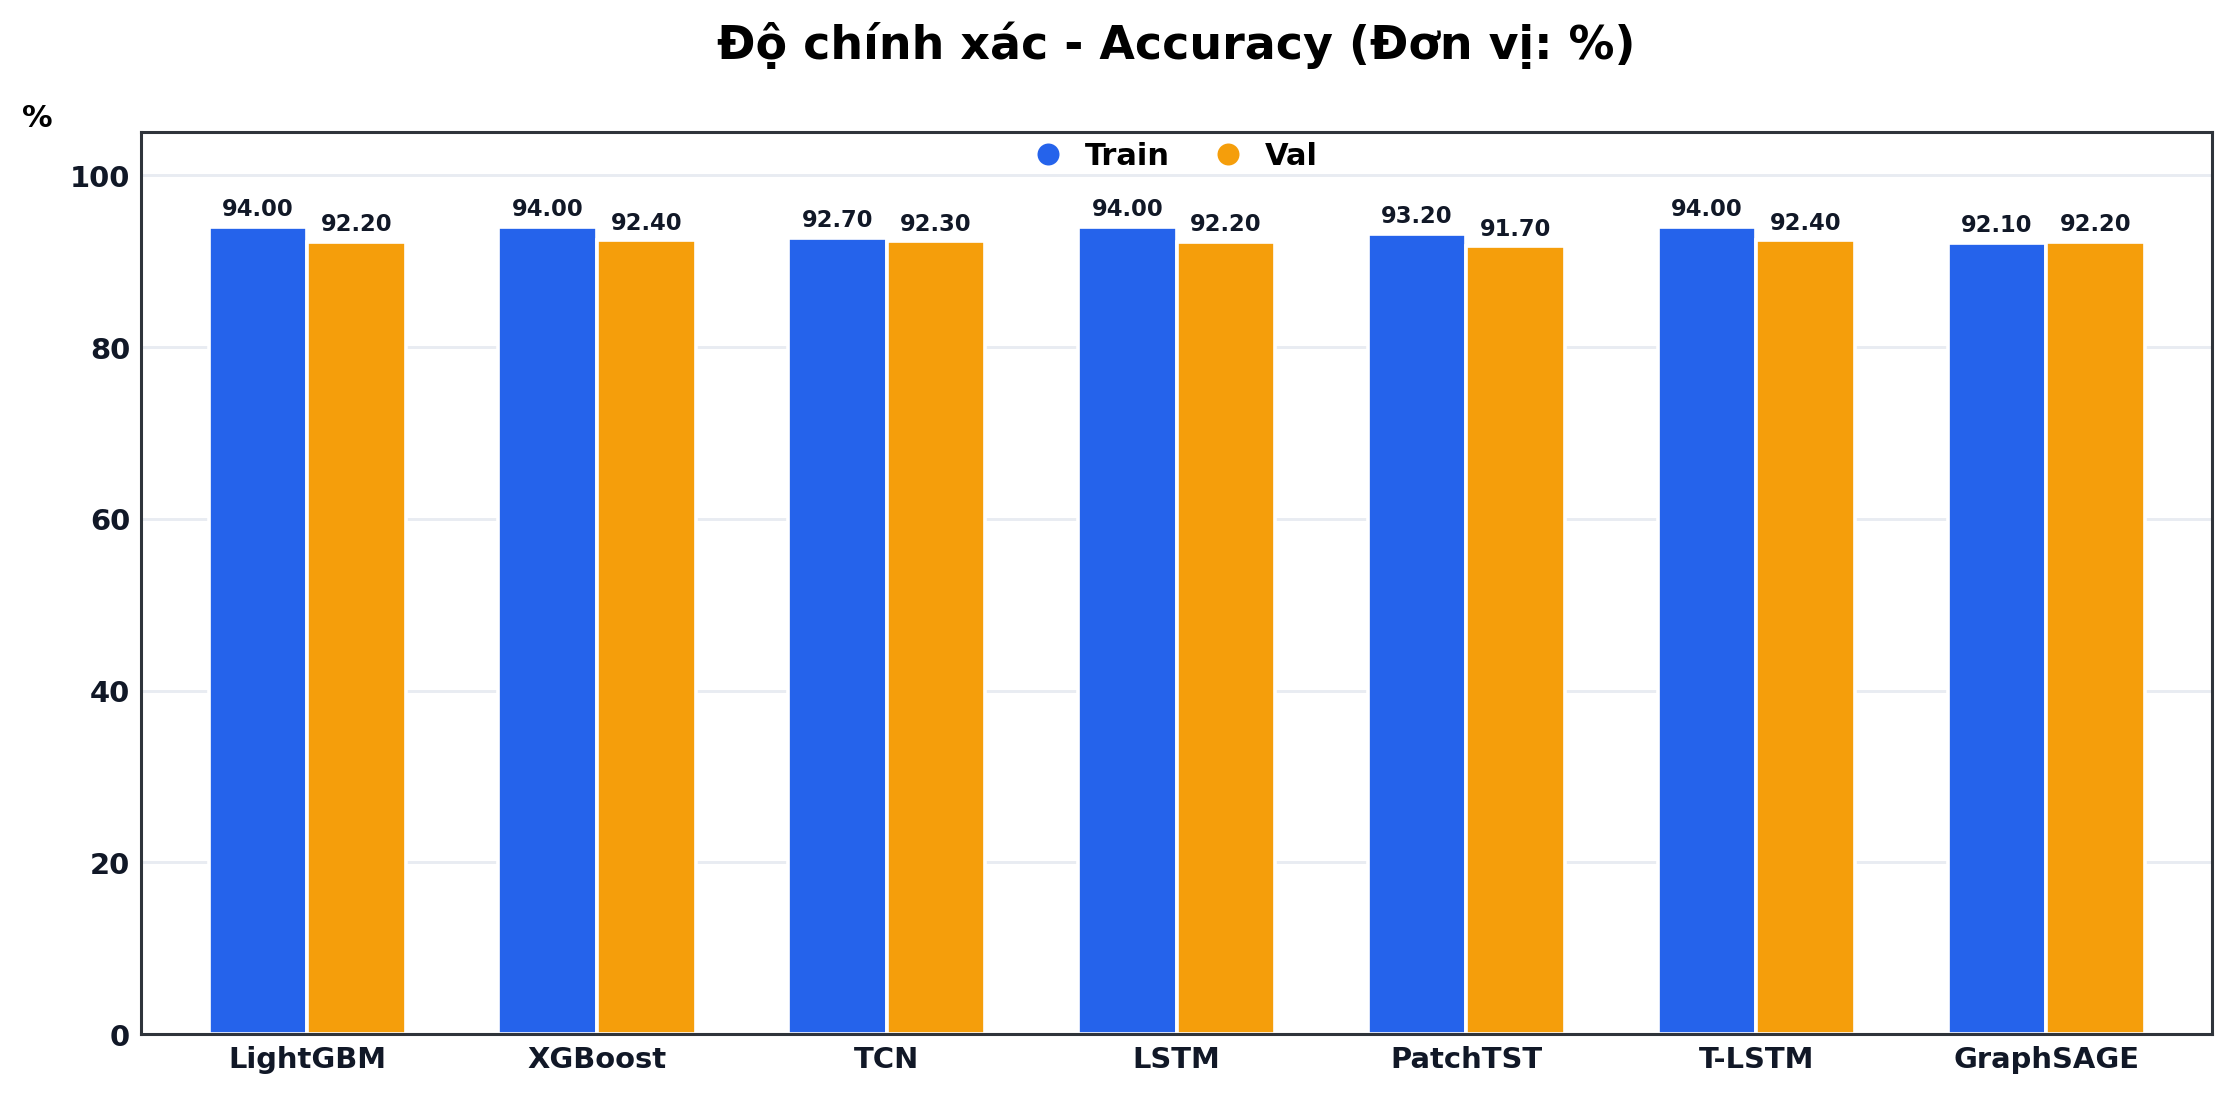
\includegraphics[width=1\textwidth]{uploads/train_val_accuracy_comparison.png}  
    \caption{Biểu đồ độ chính xác} % Dòng chú thích dưới ảnh
    \label{tab:acc-train}
\end{figure}
Hình~\ref{tab:acc-train} cho thấy Accuracy trên tập huấn luyện nằm trong khoảng 92,10\%--94,00\%, còn trên tập xác thực nằm trong khoảng 91,70\%--92,40\%. XGBoost và T-LSTM cùng đạt Accuracy xác thực cao nhất, ở mức 92,40\%. TCN và GraphSAGE có chênh lệch giữa hai tập lần lượt là 0,40 và 0,10 điểm phần trăm. PatchTST đạt Accuracy xác thực thấp nhất với 91,70\%. Khoảng biến thiên 0,70 điểm phần trăm cho thấy khác biệt giữa các mô hình trên tập xác thực tương đối nhỏ.

\begin{table}[!htbp]
\centering
\caption{Độ chính xác các kịch bản}
\label{tab:accuracy_models}

\renewcommand{\arraystretch}{1.05}
\setlength{\tabcolsep}{0pt}

\begin{tabular}{>{\centering\arraybackslash}p{0.48\textwidth}|
                >{\centering\arraybackslash}p{0.48\textwidth}}
\hline

\textbf{Kịch bản 1: LightGBM} &
\textbf{Kịch bản 2: XGBoost} \\
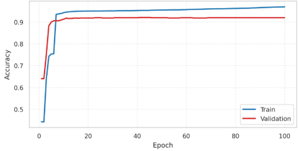
\includegraphics[width=0.85\linewidth]{acc-loss/acc-lightgbm.png} &
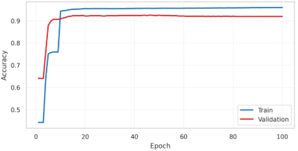
\includegraphics[width=0.85\linewidth]{acc-loss/acc-xgboost.png} \\
\hline

\textbf{Kịch bản 3: TCN} &
\textbf{Kịch bản 4: LSTM} \\
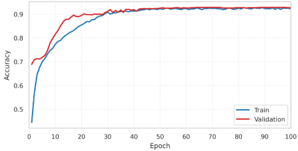
\includegraphics[width=0.85\linewidth]{acc-loss/acc-tcn.png} &
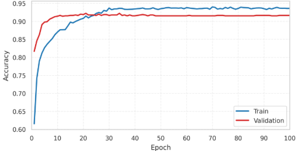
\includegraphics[width=0.85\linewidth]{acc-loss/acc-lstm.png} \\
\hline

\textbf{Kịch bản 5: PatchTST} &
\textbf{Kịch bản 6: T-LSTM} \\
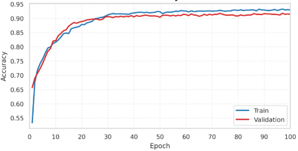
\includegraphics[width=0.85\linewidth]{acc-loss/acc-patchtst.png} &
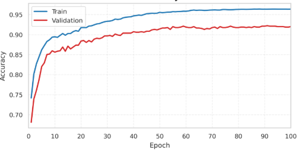
\includegraphics[width=0.85\linewidth]{acc-loss/acc-tlstm.png} \\
\hline

\textbf{Kịch bản 7: GraphSAGE} &
 \\
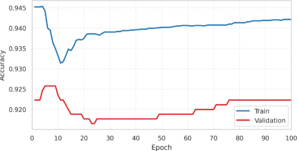
\includegraphics[width=0.85\linewidth]{acc-loss/acc-graph.png} &
 \\
\hline

\end{tabular}
\end{table}

\subsubsection{Hàm mất mát (loss)}
\begin{figure}[!htbp]
    \centering % Căn giữa hình ảnh
    
\includegraphics[width=1\textwidth]{acc-loss/train_val_loss_comparison.png} 
    \caption{Biểu đồ độ mất mát} % Dòng chú thích dưới ảnh
\end{figure}

Hàm mất mát trên tập huấn luyện dao động từ 0,123 đến 0,343; trên tập xác thực, giá trị này dao động từ 0,223 đến 0,399. T-LSTM có hàm mất mát xác thực thấp nhất (0,223), tiếp theo là LightGBM (0,266), XGBoost (0,267) và LSTM (0,268). GraphSAGE ghi nhận giá trị cao nhất trên cả tập huấn luyện (0,343) và tập xác thực (0,399). Các kết quả mô tả này cho thấy T-LSTM duy trì giá trị hàm mất mát thấp trên tập xác thực, nhưng chưa đủ để kết luận khác biệt có ý nghĩa thống kê giữa các mô hình.

\begin{table}[!htbp]
\centering
\caption{Độ mất mát các kịch bản}
\label{tab:loss_models}

\renewcommand{\arraystretch}{1.05}
\setlength{\tabcolsep}{0pt}

\begin{tabular}{>{\centering\arraybackslash}p{0.48\textwidth}|
                >{\centering\arraybackslash}p{0.48\textwidth}}
\hline

\textbf{Kịch bản 1: LightGBM} &
\textbf{Kịch bản 2: XGBoost} \\
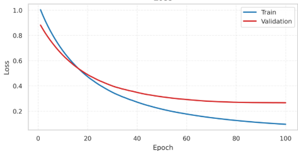
\includegraphics[width=0.75\linewidth]{acc-loss/loss-lightgbm.png} &
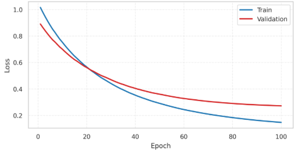
\includegraphics[width=0.75\linewidth]{acc-loss/loss-xgboost.png} \\
\hline

\textbf{Kịch bản 3: TCN} &
\textbf{Kịch bản 4: LSTM} \\
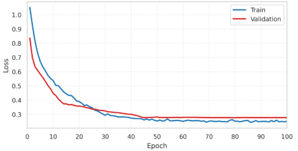
\includegraphics[width=0.75\linewidth]{acc-loss/loss-tcn.png} &
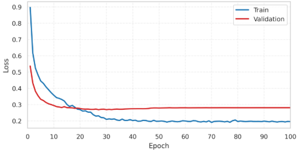
\includegraphics[width=0.75\linewidth]{acc-loss/loss-lstm.png} \\
\hline

\textbf{Kịch bản 5: PatchTST} &
\textbf{Kịch bản 6: T-LSTM} \\
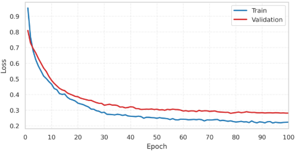
\includegraphics[width=0.75\linewidth]{acc-loss/loss-oatchtst.png} &
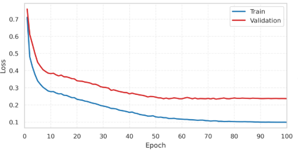
\includegraphics[width=0.75\linewidth]{acc-loss/loss-tlstm.png} \\
\hline

\textbf{Kịch bản 7: GraphSAGE} &
 \\
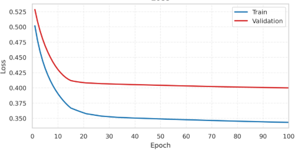
\includegraphics[width=0.75\linewidth]{acc-loss/loss-graph.png} &
 \\
\hline

\end{tabular}
\end{table}

\subsubsection{Thời gian huấn luyện}

\begin{figure}[!htbp]
    \centering % Căn giữa hình ảnh
    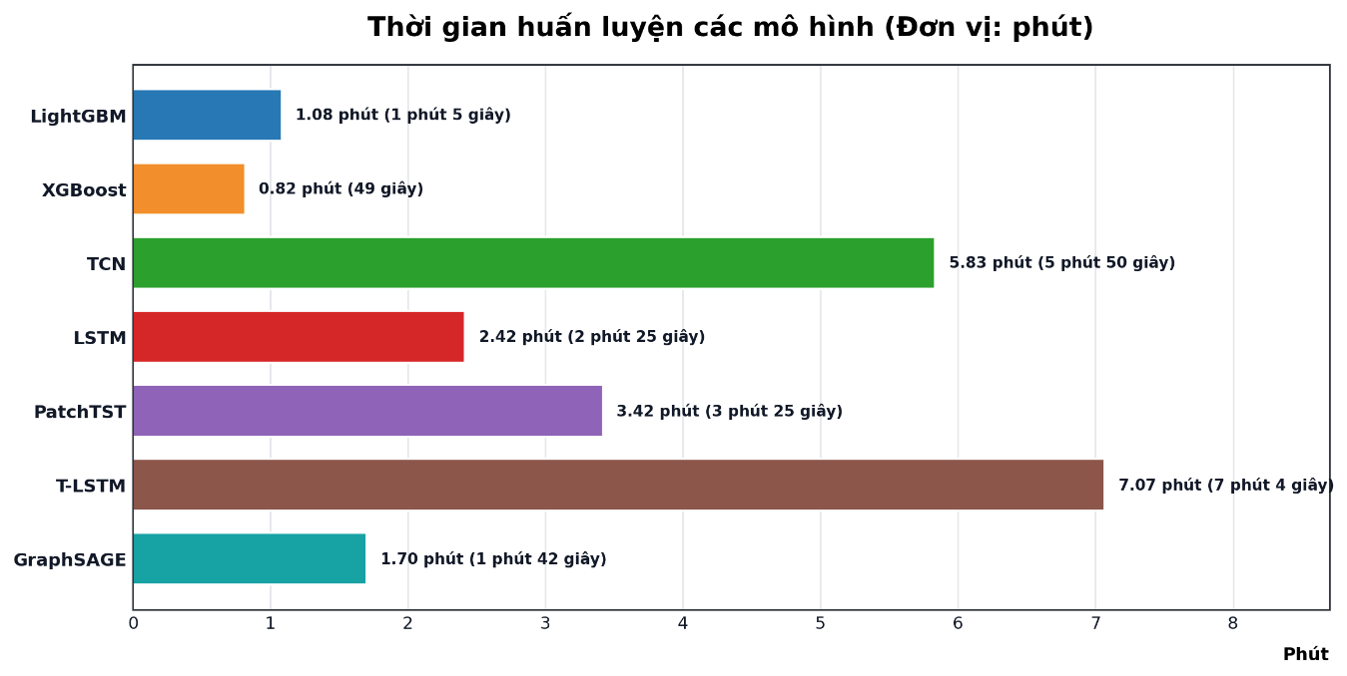
\includegraphics[width=1\textwidth]{acc-loss/time-train.png} % Thay 'ten-file-anh' bằng tên ảnh của bạn (không cần đuôi .png/.jpg)
    \caption{Thời gian huấn luyện các kịch bản } % Dòng chú thích dưới ảnh
\end{figure}
Thời gian huấn luyện khác nhau đáng kể giữa các kiến trúc. T-LSTM và TCN có thời gian cao nhất, lần lượt là 7,07 và 5,83 phút. PatchTST, LSTM và GraphSAGE lần lượt cần 3,42, 2,42 và 1,70 phút; XGBoost và LightGBM cần 0,82 và 1,08 phút. Kết quả phản ánh sự đánh đổi giữa chi phí huấn luyện của các mô hình chuỗi và tốc độ của các mô hình cây tăng cường trong môi trường thực nghiệm đã sử dụng.

\subsection{Kết quả kiểm thử}

\subsubsection{Độ chính xác}
\begin{figure}[!htbp]
    \centering % Căn giữa hình ảnh
    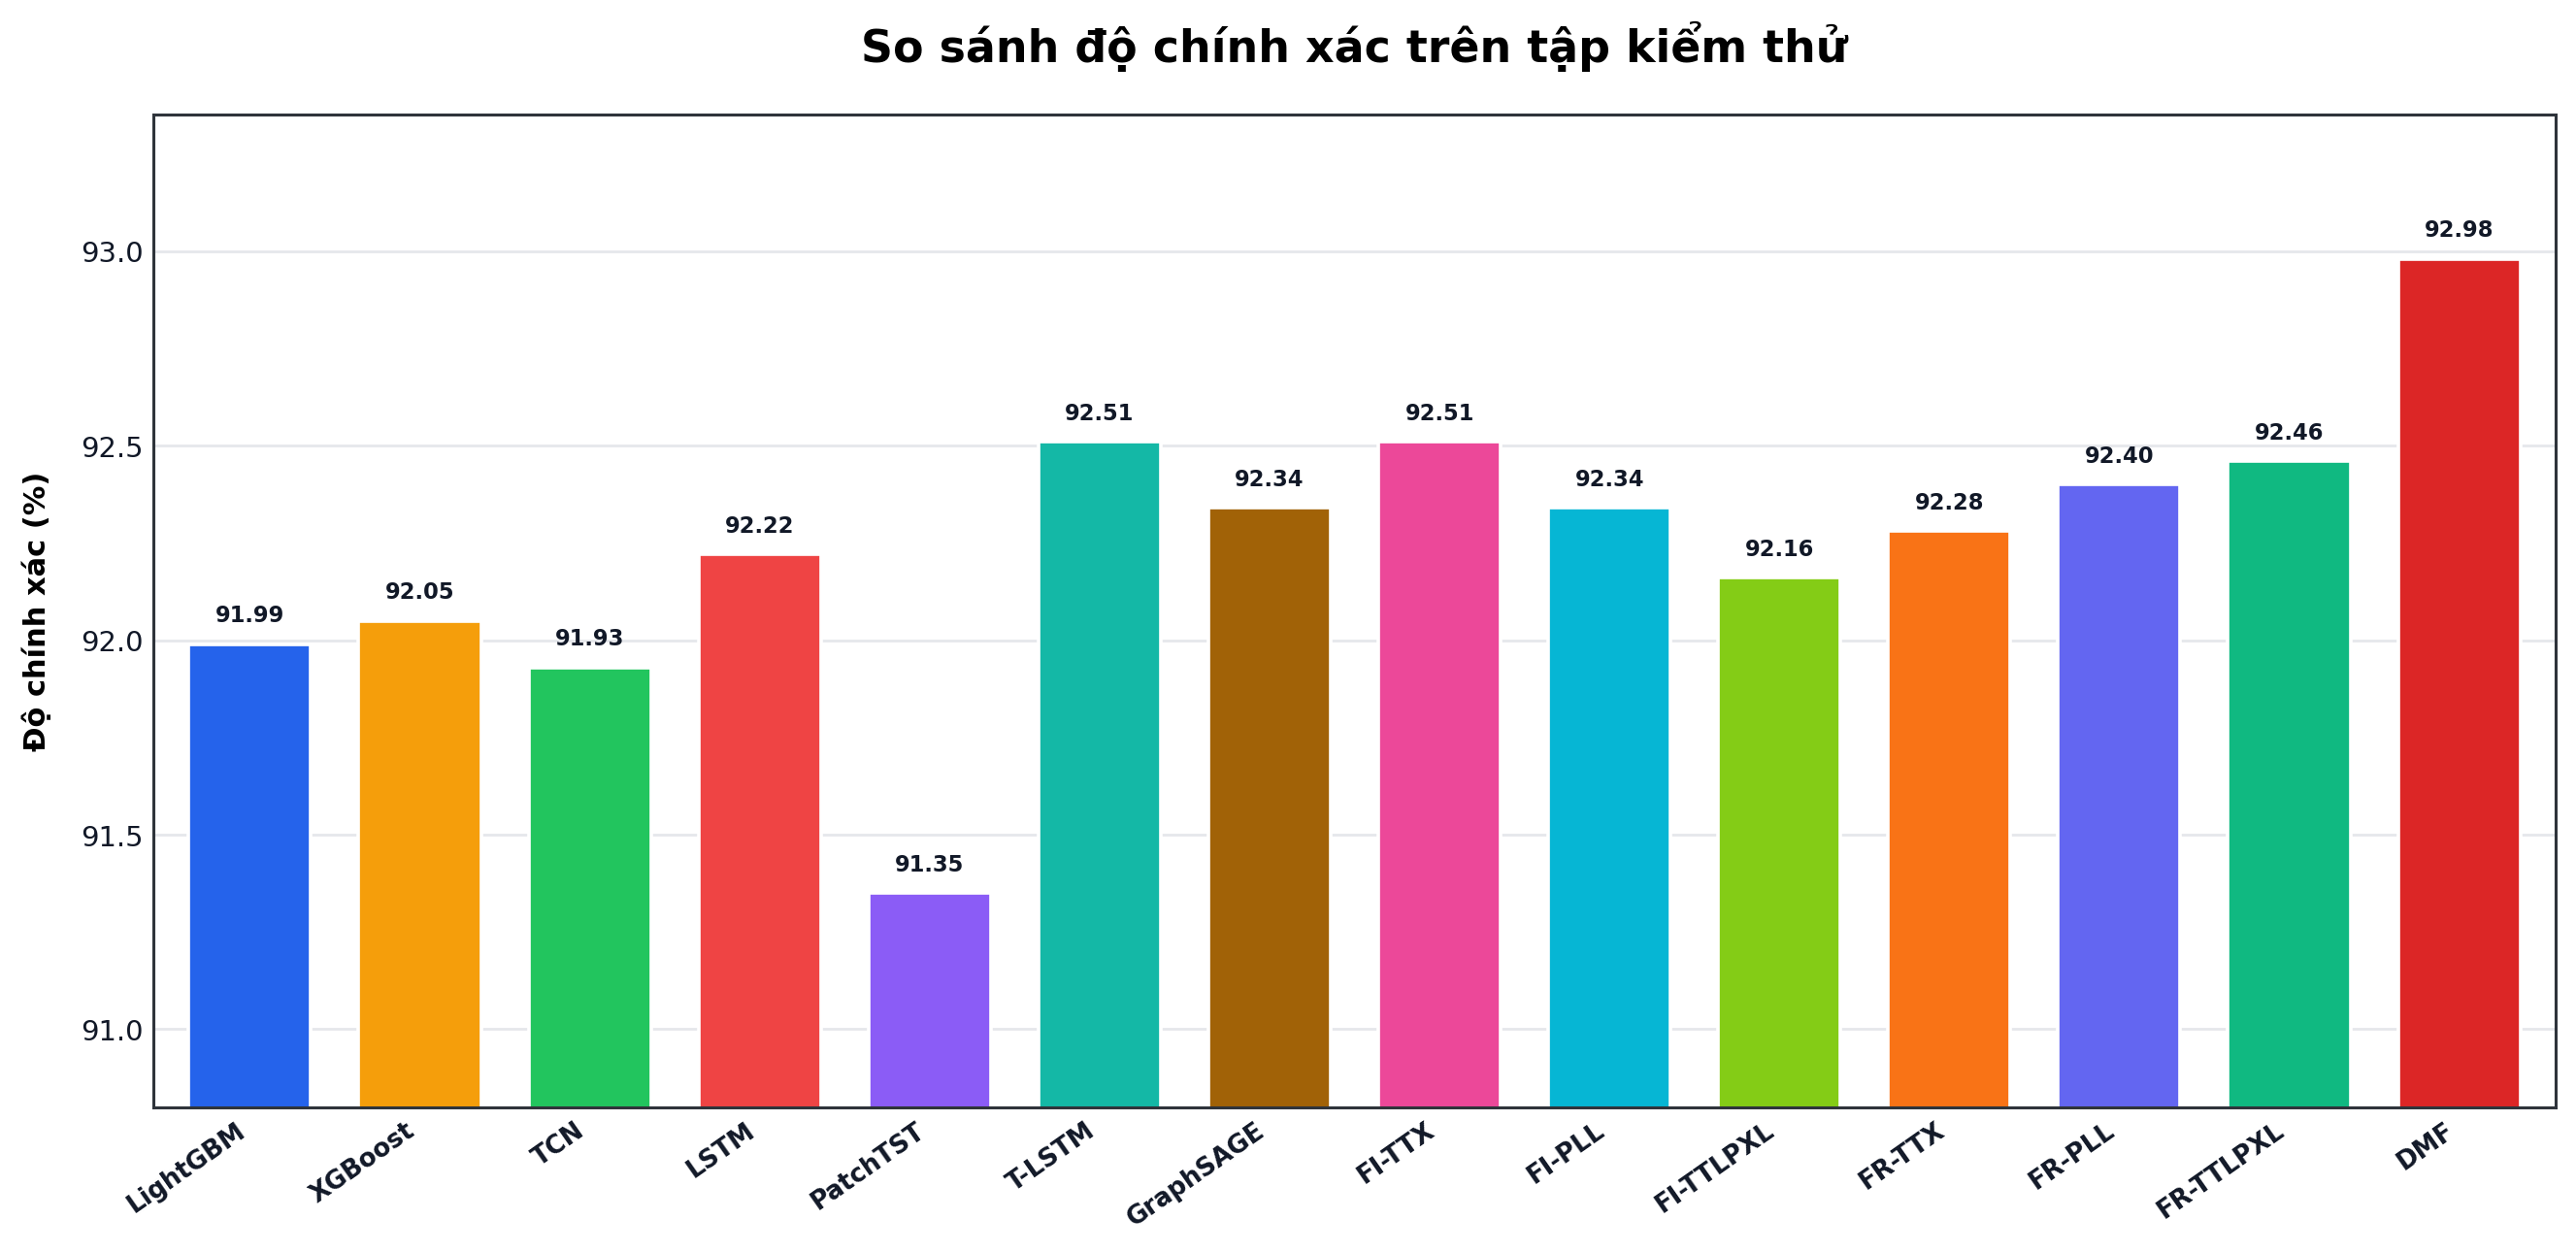
\includegraphics[width=1\textwidth]{acc-loss/test_accuracy_scenario_comparison.png} 
    \caption{Biểu đồ độ chính xác trên tập kiểm thử} 
    \label{tab:acc-test}
\end{figure}
Accuracy trên tập kiểm thử nằm trong khoảng 91,35\%--92,98\%. Trong nhóm mô hình riêng lẻ, T-LSTM đạt giá trị cao nhất (92,51\%), tiếp theo là GraphSAGE (92,34\%) và LSTM (92,22\%). FI-TTX cũng đạt 92,51\%, còn FR-TTLPXL đạt 92,46\%. DMF có Accuracy cao nhất trong 14 kịch bản, ở mức 92,98\%. Kết quả này ghi nhận lợi ích tiềm năng của cơ chế lựa chọn động; tuy nhiên, cần kiểm định bổ sung để xác định ý nghĩa thống kê của mức chênh lệch.

\subsubsection{Precision của các kịch bản}

\begin{figure}[!htbp]
\centering


\captionsetup[subfigure]{
    labelformat=simple,
    labelsep=period,
    font=it,
    justification=centering
}

\renewcommand{\thesubfigure}{\alph{subfigure}}

\begin{subfigure}{0.92\textwidth}
    \centering
    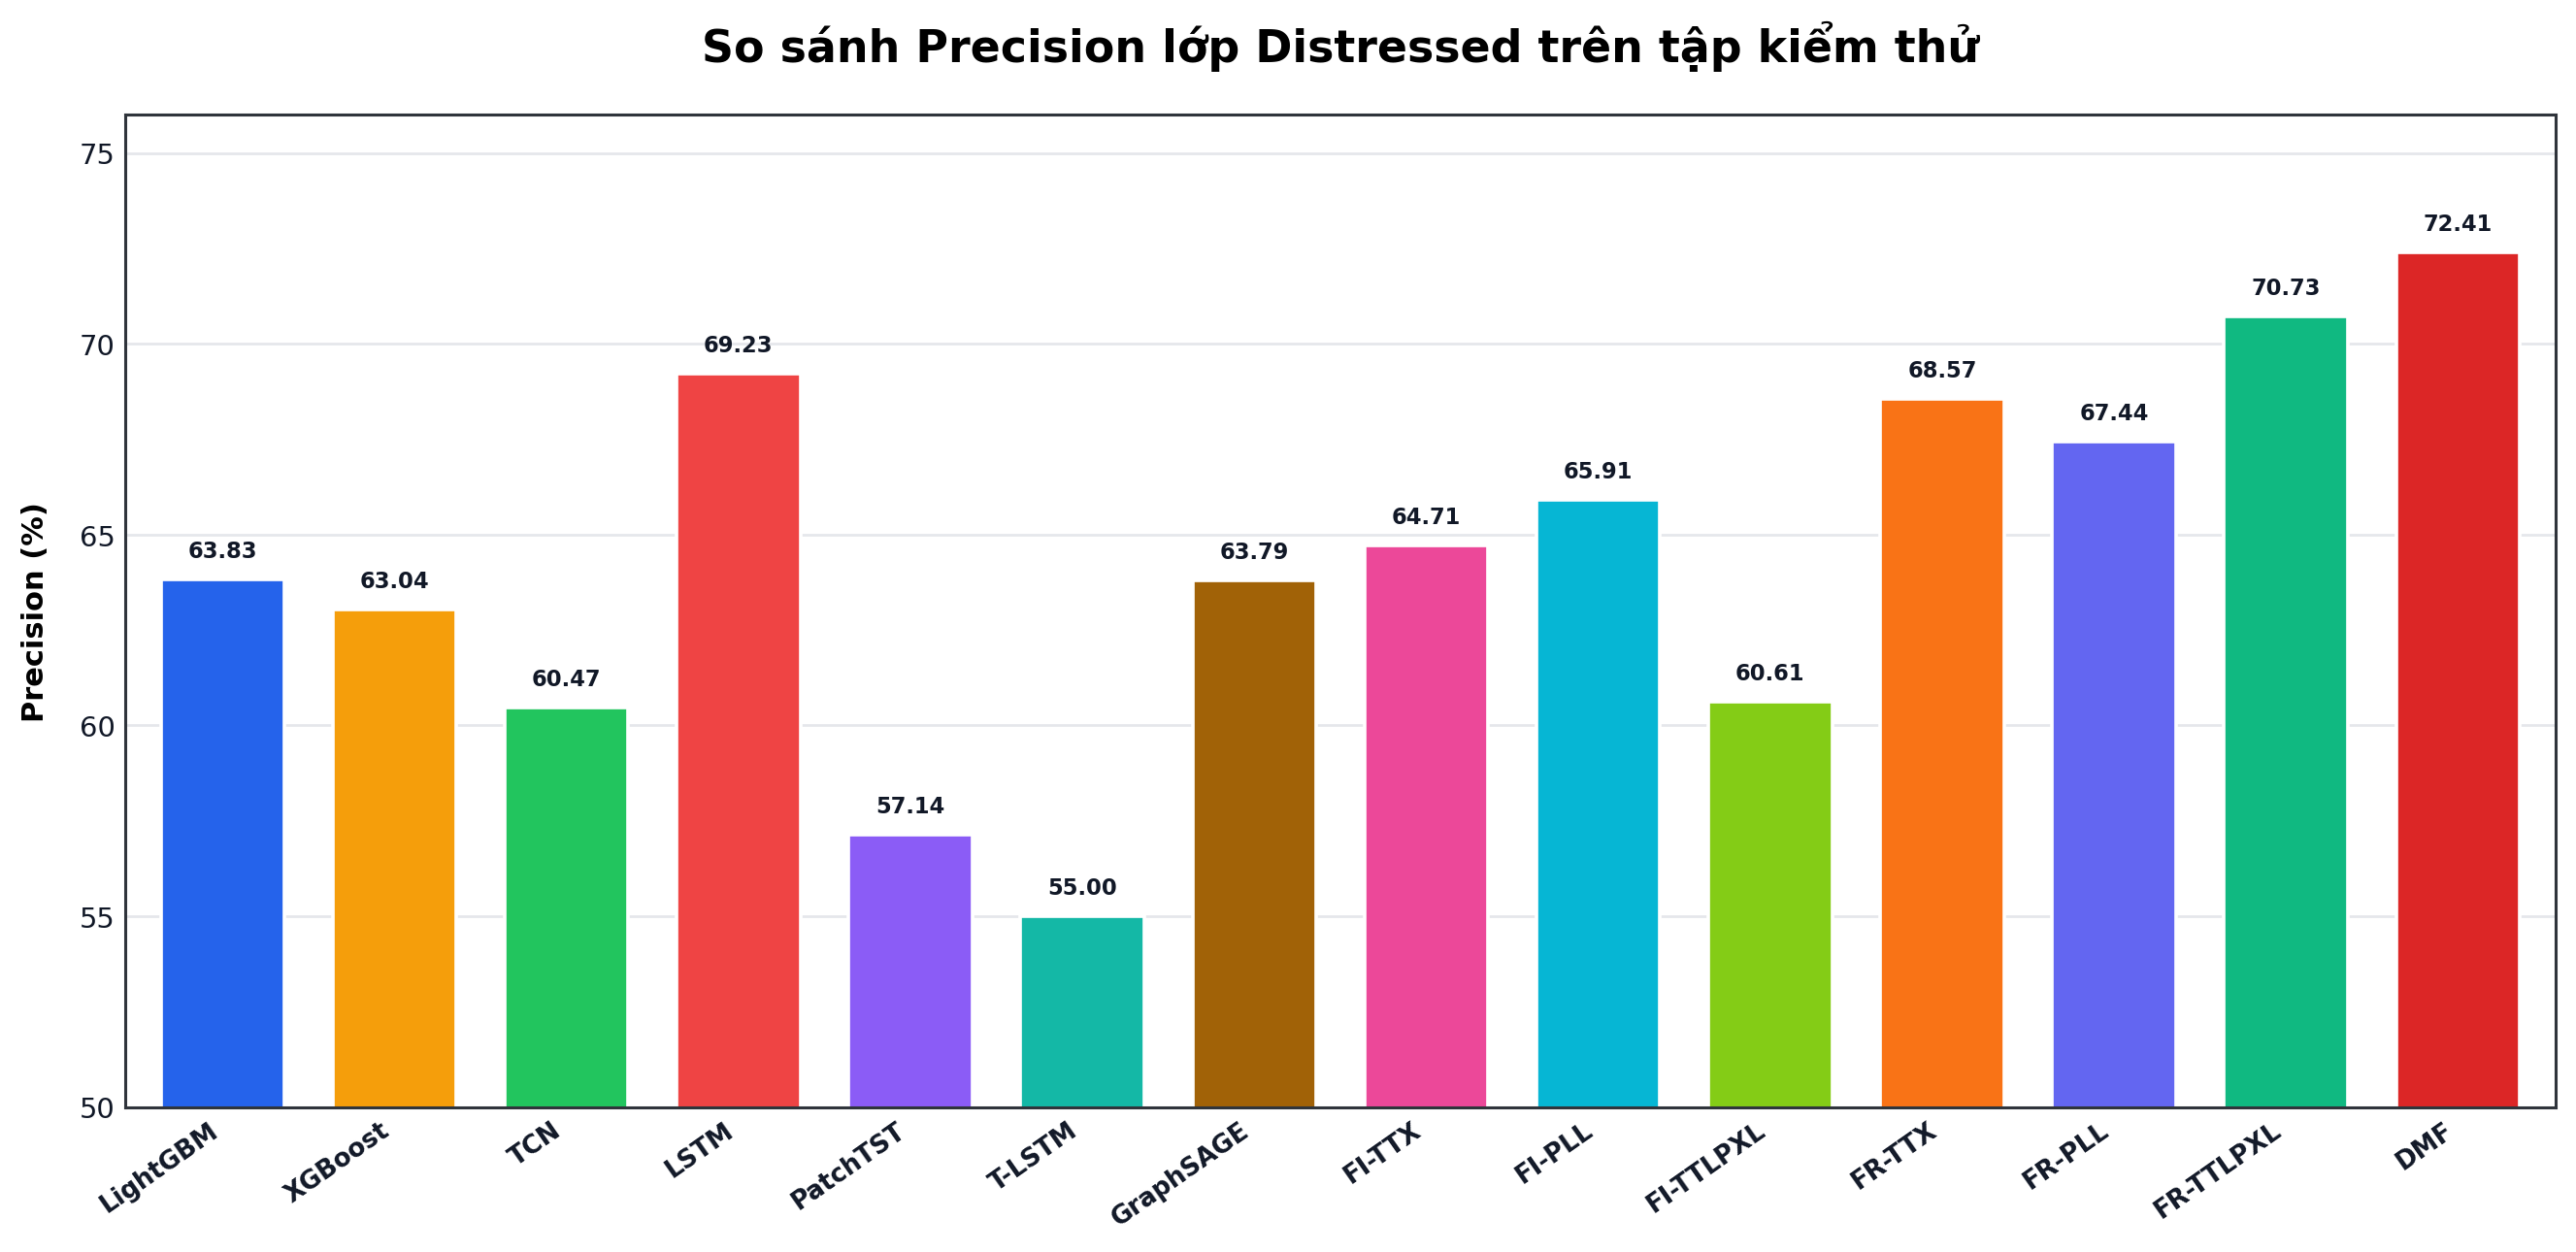
\includegraphics[width=\textwidth]{acc-loss/distressed_precision_test_comparison.png}
    \caption{Precision của lớp Distressed}
    \label{fig:precision_distressed}
\end{subfigure}

\vspace{0.15cm}

\begin{subfigure}{0.92\textwidth}
    \centering
    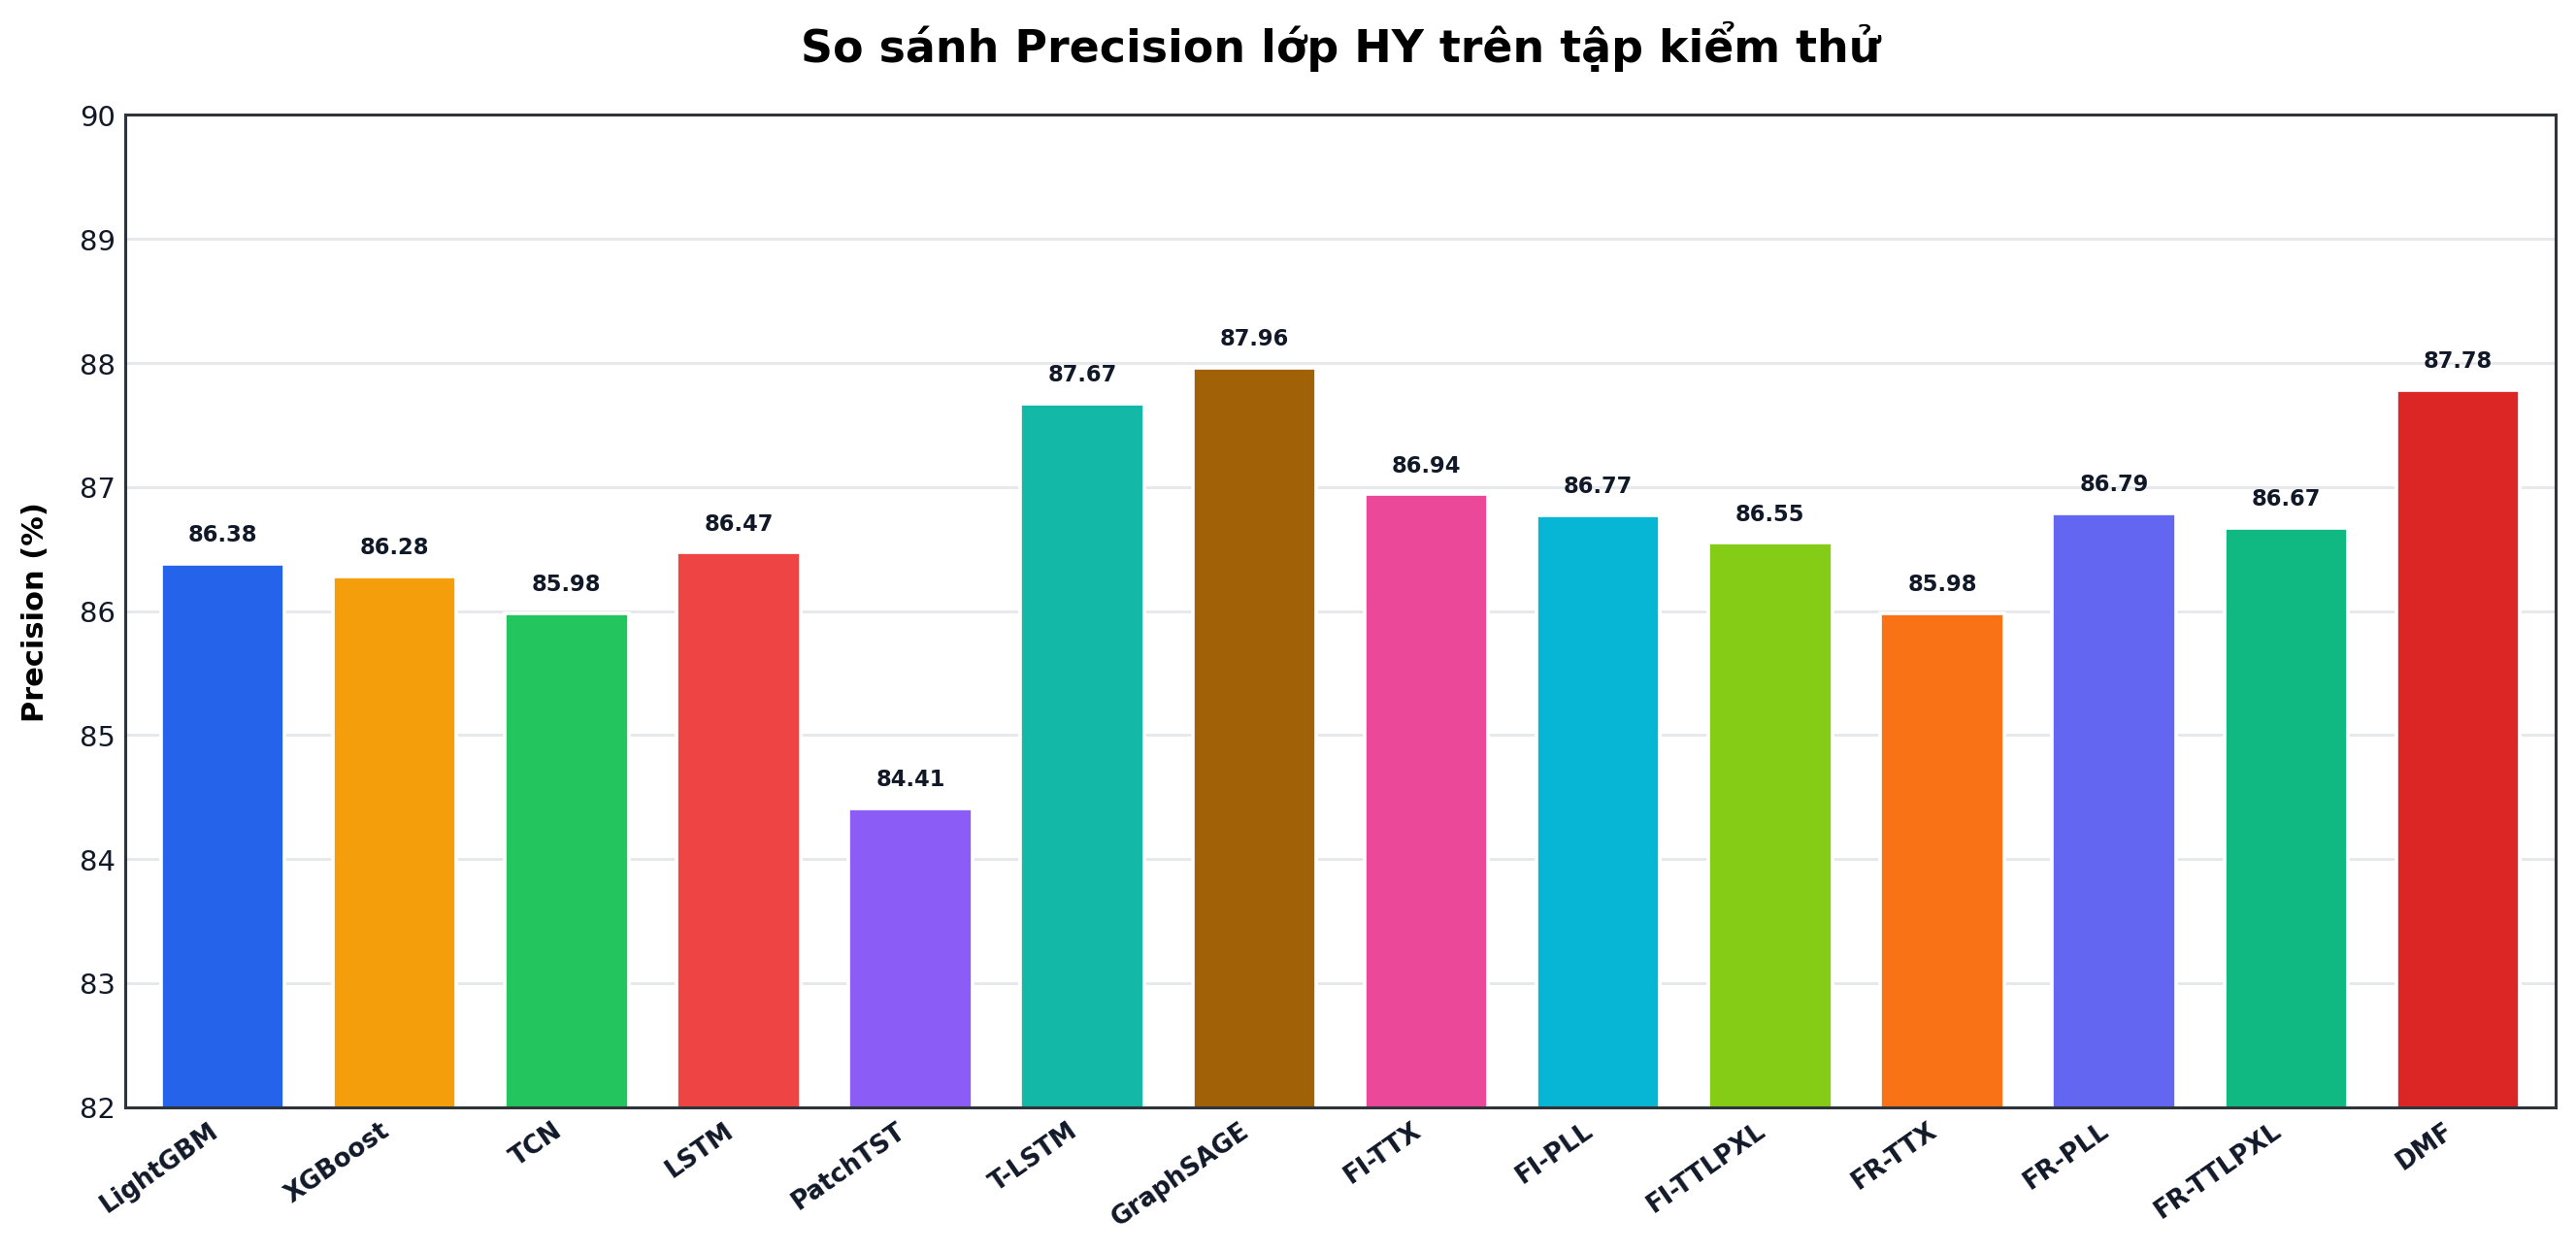
\includegraphics[width=\textwidth]{acc-loss/hy_precision_test_comparison.png}
    \caption{Precision của lớp HY (High Yield)}
    \label{fig:precision_hy}
\end{subfigure}

\vspace{0.15cm}

\begin{subfigure}{0.92\textwidth}
    \centering
    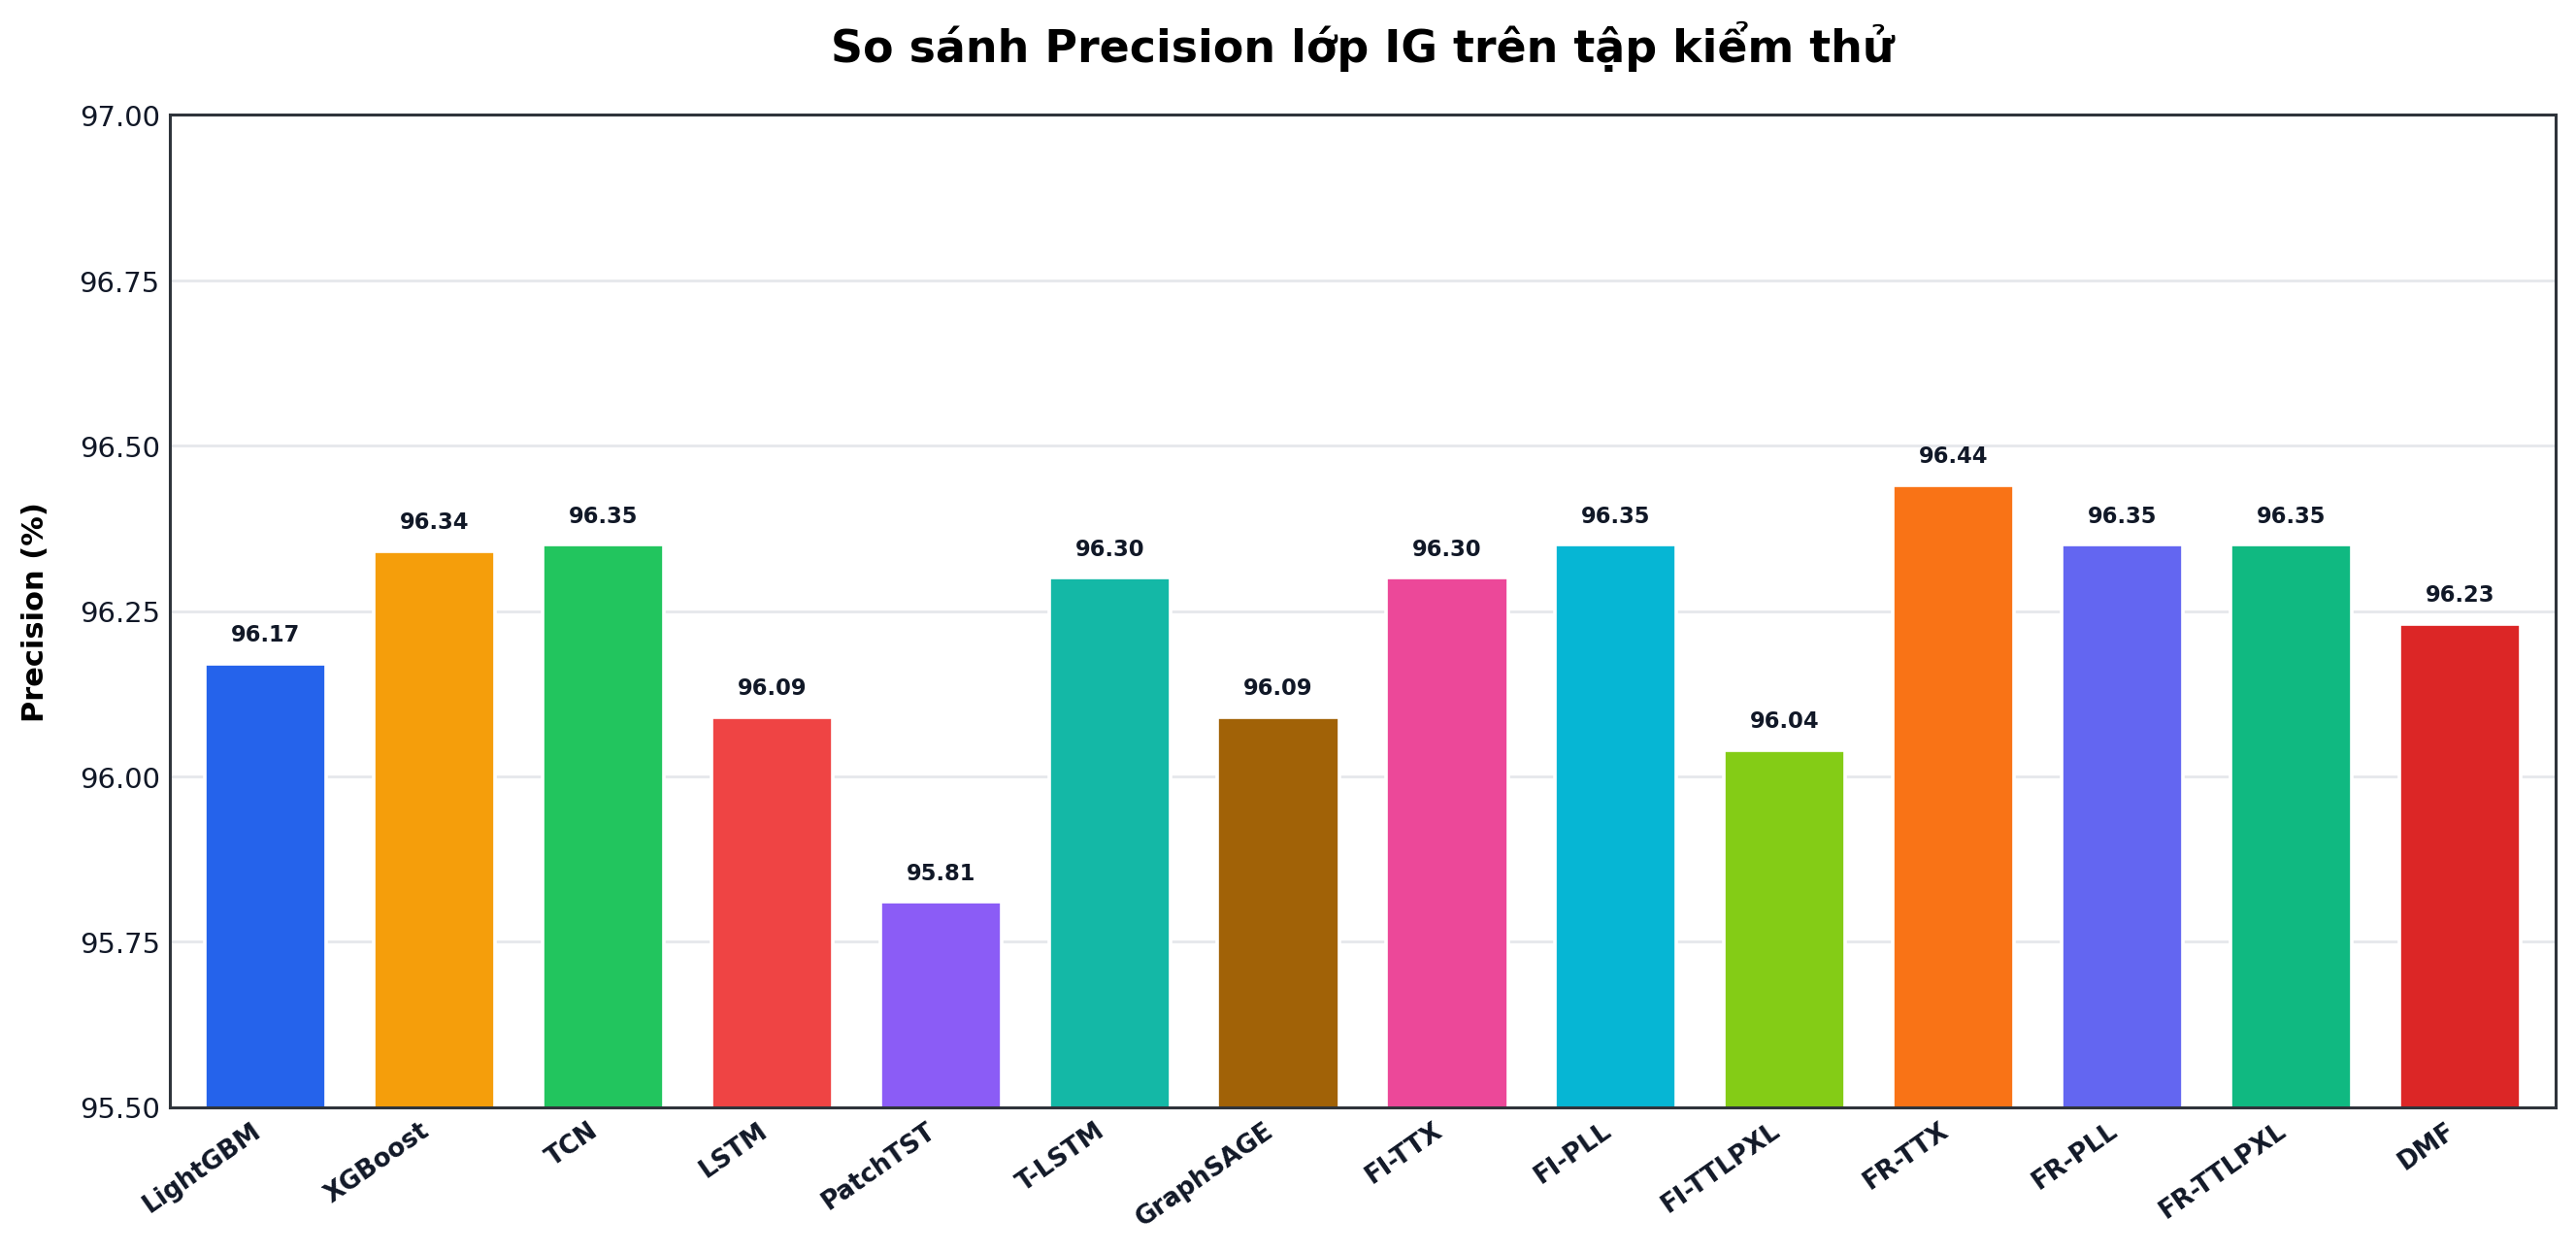
\includegraphics[width=\textwidth]{acc-loss/ig_precision_test_comparison.png}
    \caption{Precision của lớp IG (Investment Grade)}
    \label{fig:precision_ig}
\end{subfigure}
\label{fig:precision_classes}

\caption{Precision lớp Distressed (a), lớp HY (b) và lớp IG (c) trên tập kiểm thử }
\end{figure}
Precision thay đổi theo từng lớp xếp hạng. Với lớp Distressed, DMF đạt giá trị cao nhất (72,41\%), tiếp theo là FR-TTLPXL (70,73\%) và LSTM (69,23\%). Với lớp HY, Precision nằm trong khoảng 84,41\%--87,96\%; GraphSAGE đạt 87,96\%, DMF đạt 87,78\% và T-LSTM đạt 87,67\%. Đối với lớp IG, các giá trị nằm trong khoảng 95,81\%--96,44\%, trong đó FR-TTX đạt mức cao nhất. Chênh lệch giữa các lớp cho thấy Precision tổng thể cần được đọc cùng các chỉ số theo lớp, đặc biệt đối với nhóm Distressed.

\subsubsection{Recall của các kịch bản}
\begin{figure}[!htbp]
\centering


\captionsetup[subfigure]{
    labelformat=simple,
    labelsep=period,
    font=it,
    justification=centering
}

\renewcommand{\thesubfigure}{\alph{subfigure}}

\begin{subfigure}{0.92\textwidth}
    \centering
    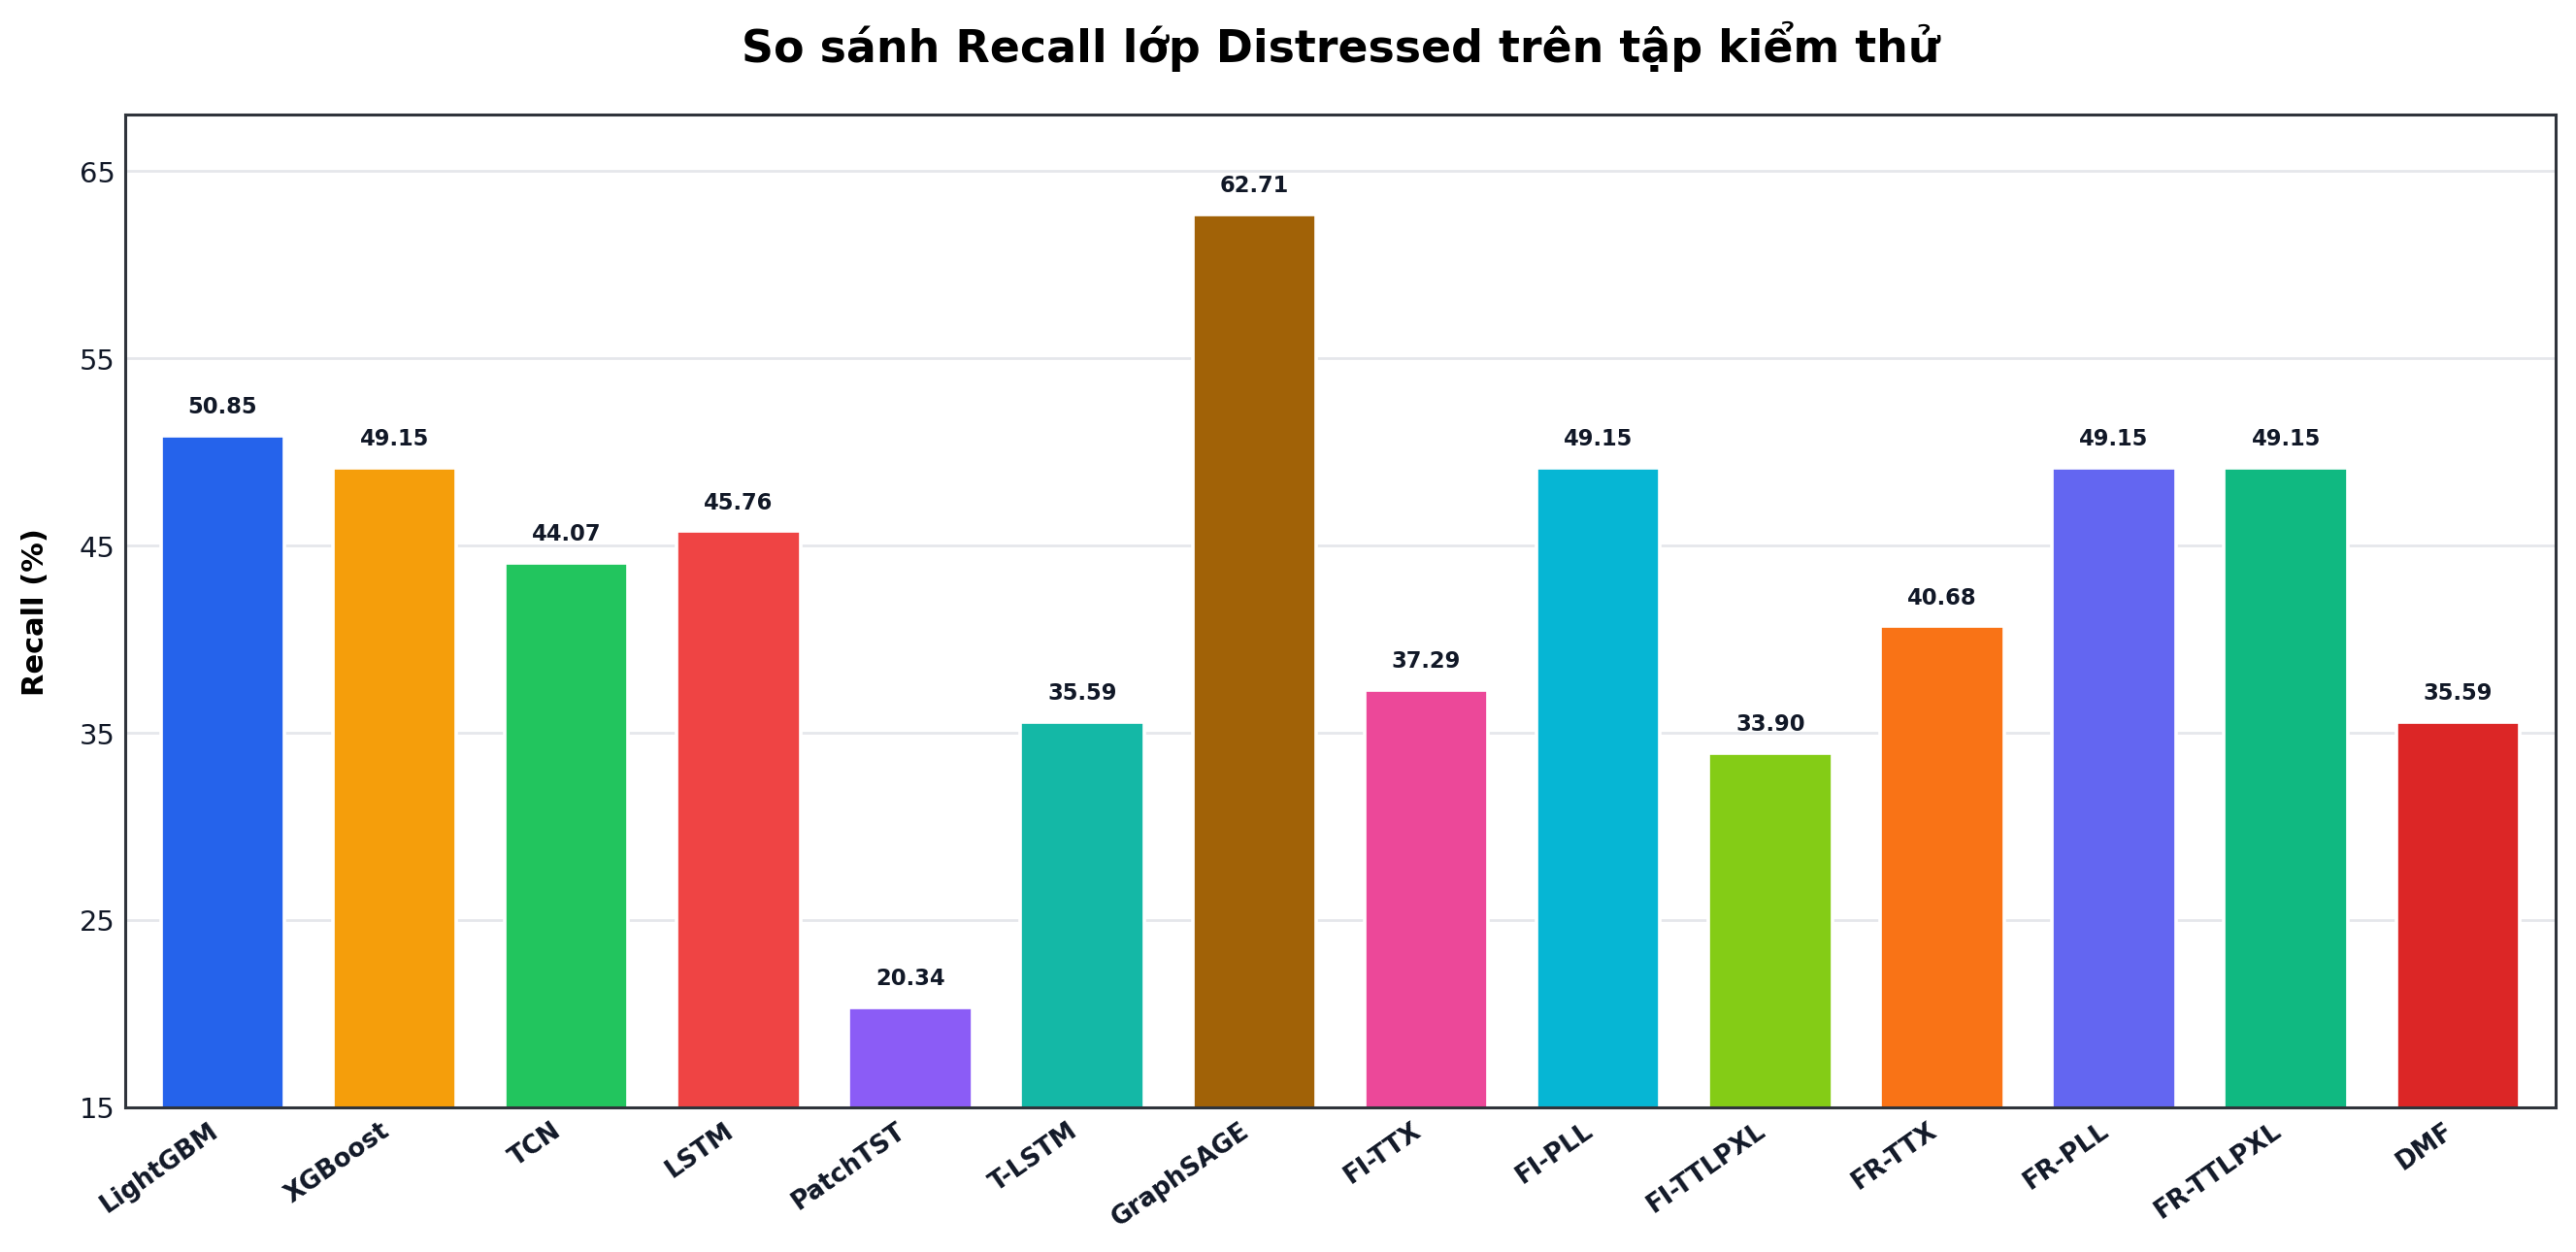
\includegraphics[width=\textwidth]{acc-loss/distressed_recall_test_comparison.png}
    \caption{Recall của lớp Distressed}
    \label{fig:Recall_distressed}
\end{subfigure}

\vspace{0.15cm}

\begin{subfigure}{0.92\textwidth}
    \centering
    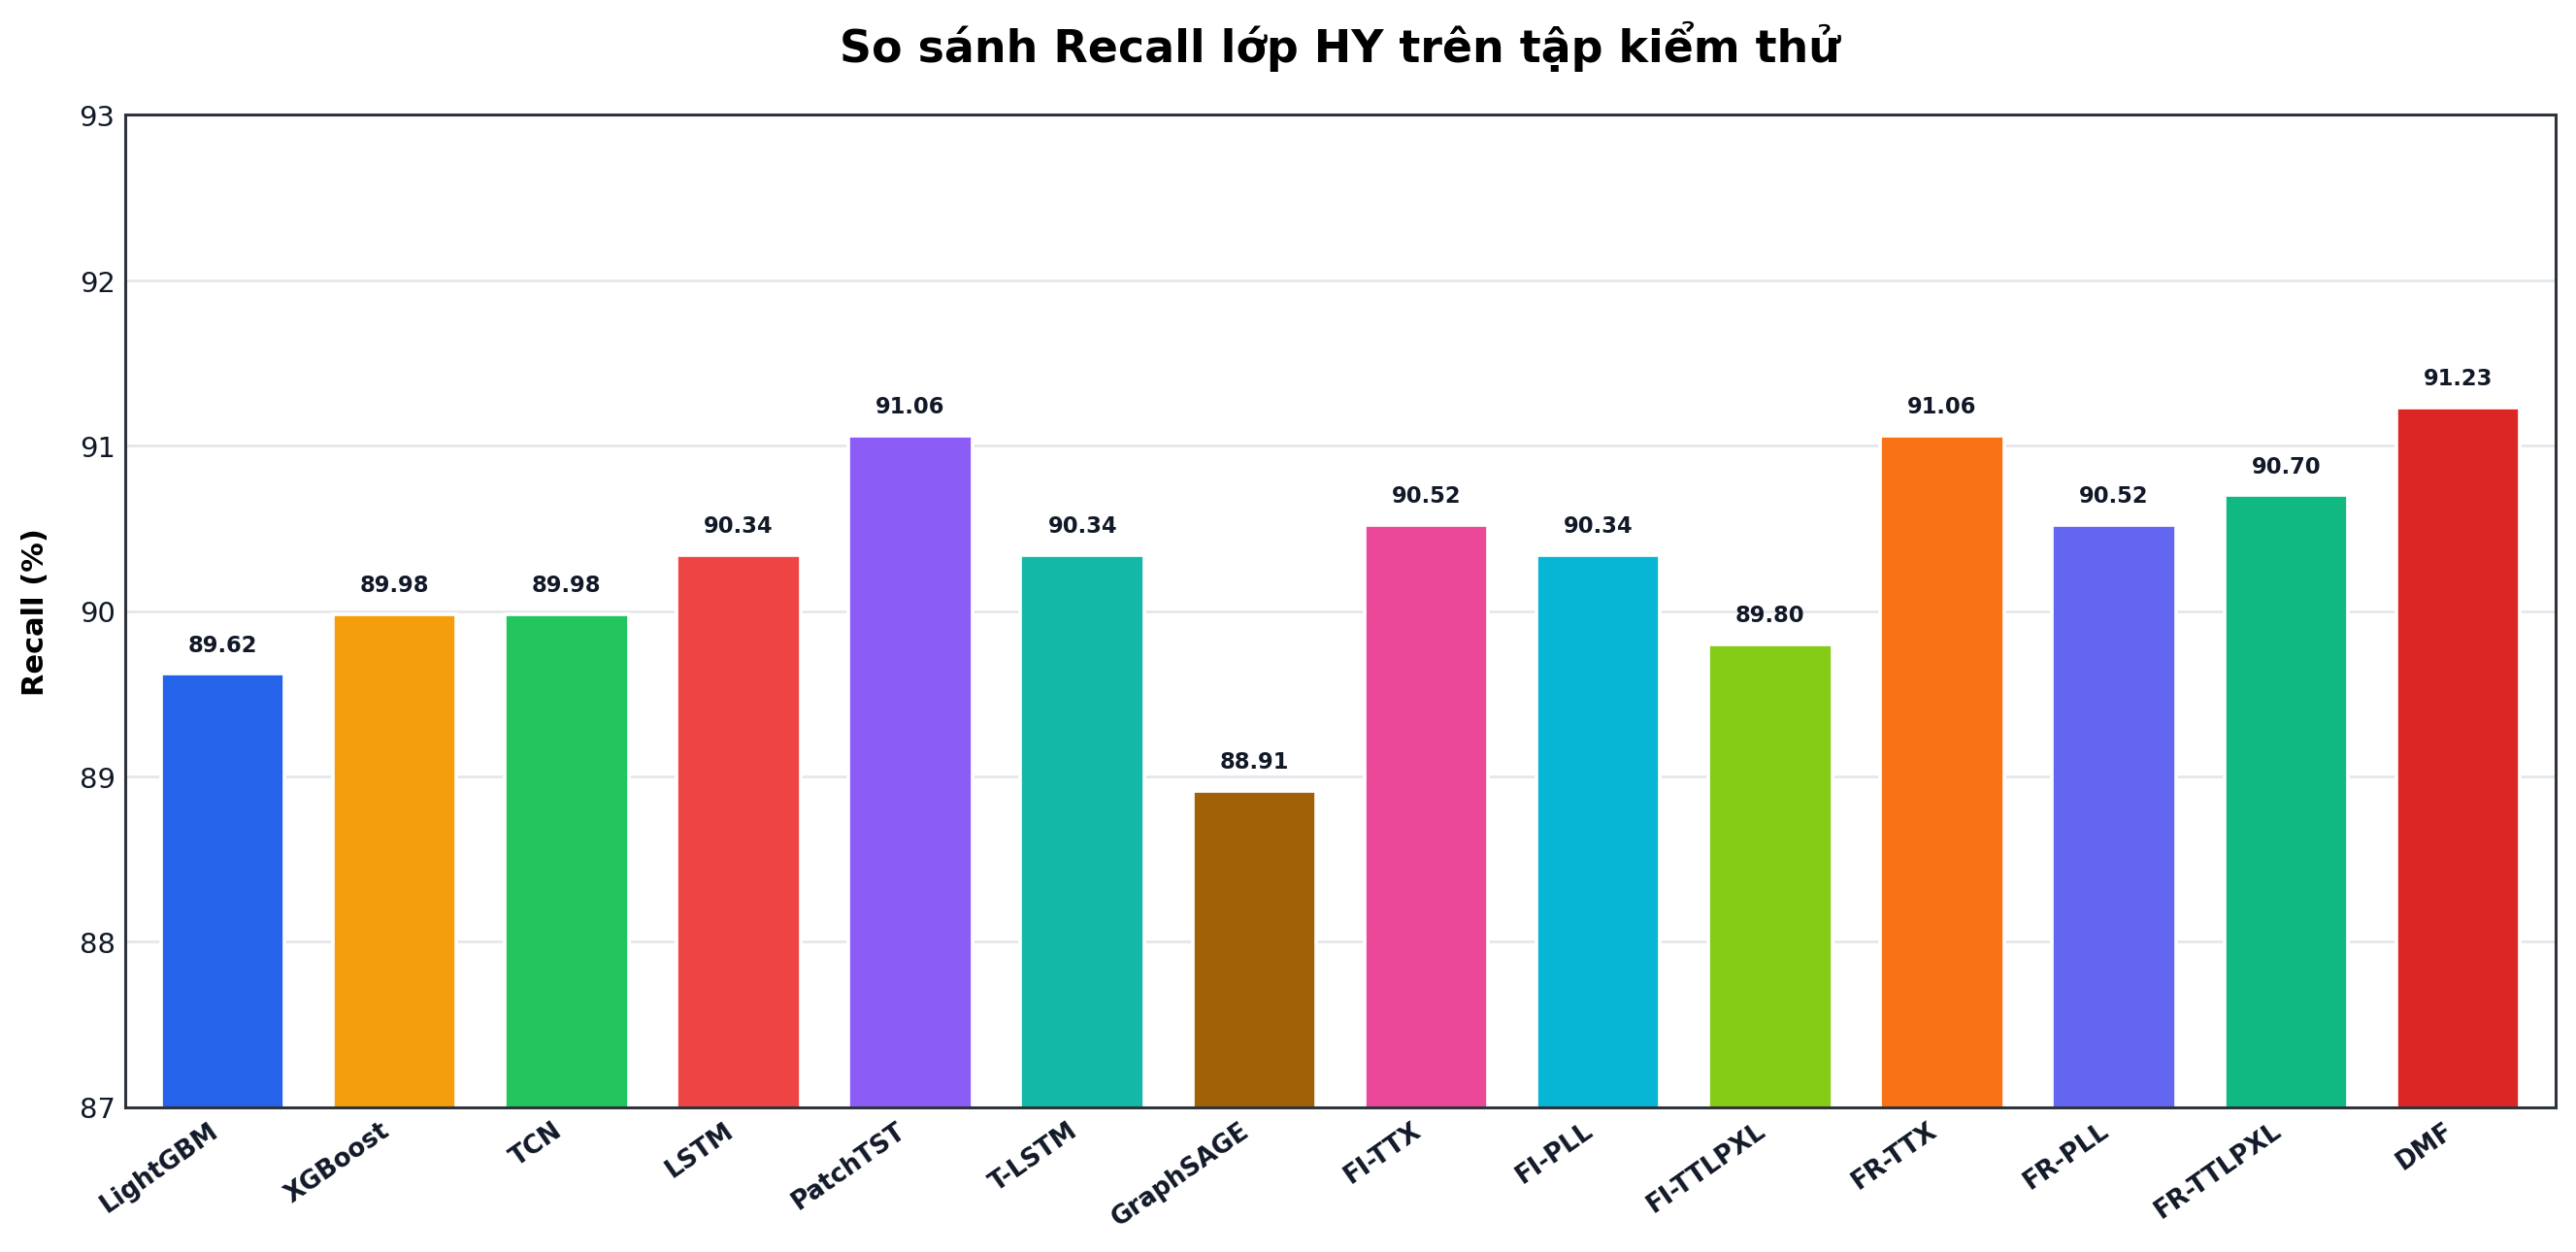
\includegraphics[width=\textwidth]{acc-loss/hy_recall_test_comparison.png}
    \caption{Recall của lớp HY (High Yield)}
    \label{fig:Recall_hy}
\end{subfigure}

\vspace{0.15cm}

\begin{subfigure}{0.92\textwidth}
    \centering
    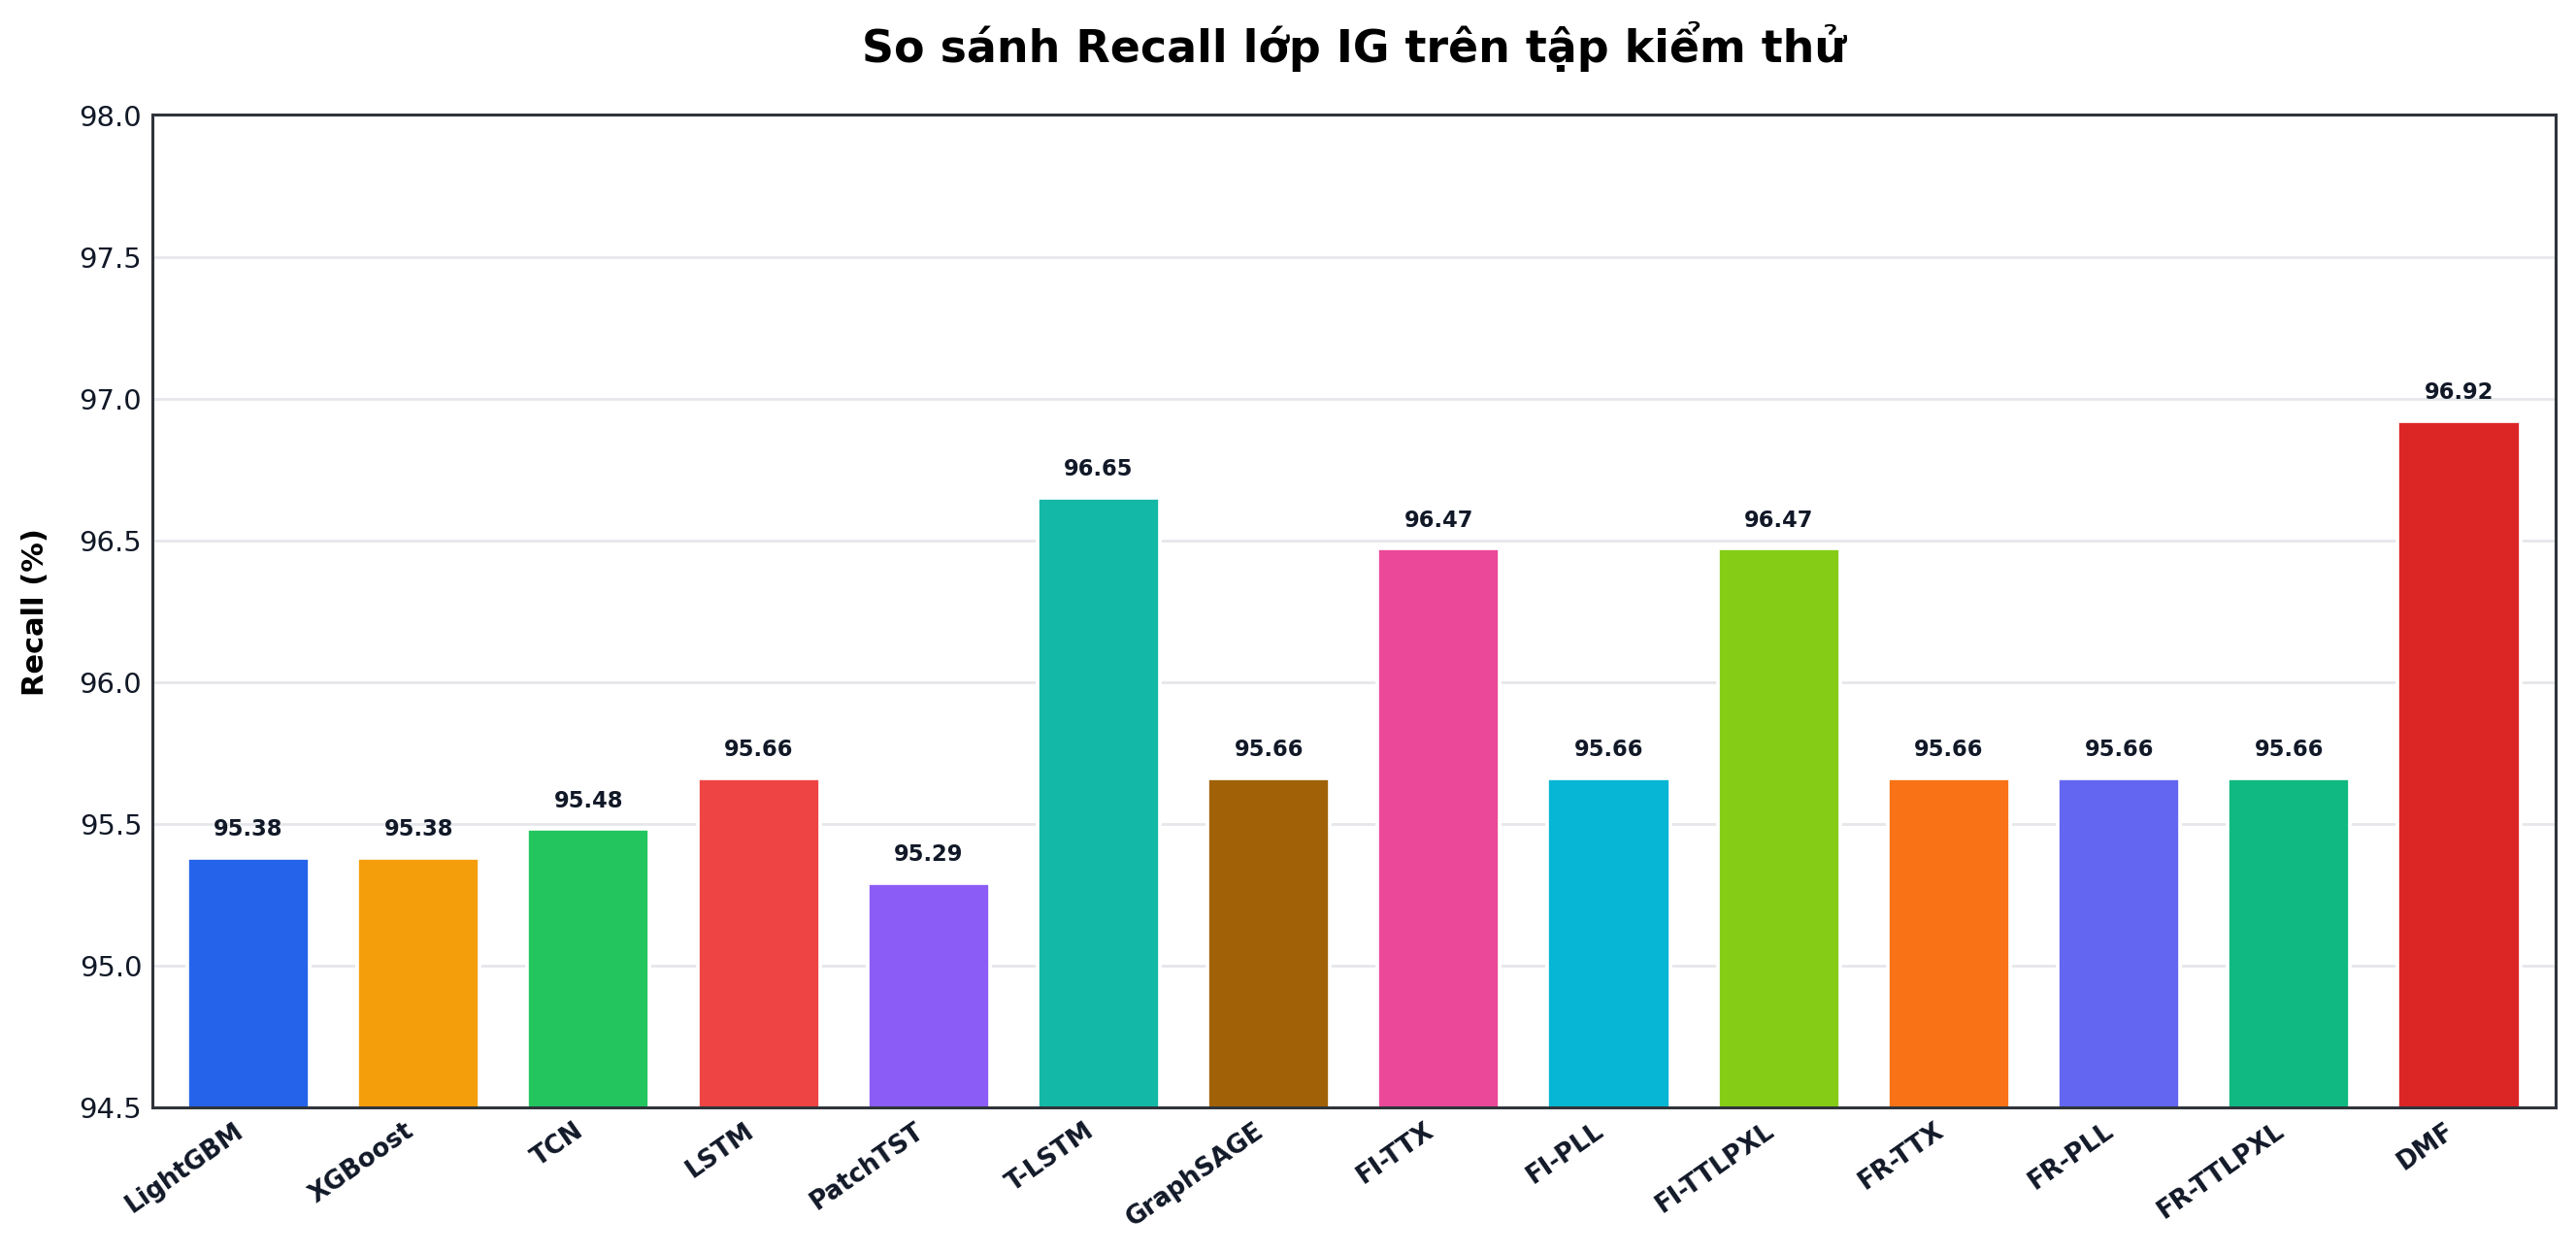
\includegraphics[width=\textwidth]{acc-loss/ig_recall_test_comparison.png}
    \caption{Recall của lớp IG (Investment Grade)}
    \label{fig:Recall_ig}
\end{subfigure}
\label{fig:Recall_classes}

\caption{Recall lớp Distressed (a), lớp HY (b) và lớp IG (c) trên tập kiểm thử }
\end{figure}
Recall thể hiện khác biệt lớn nhất ở lớp Distressed. GraphSAGE đạt Recall 62,71\%, cao hơn LightGBM (50,85\%), XGBoost (49,15\%) và DMF (35,59\%); PatchTST đạt giá trị thấp nhất với 20,34\%. Ở lớp HY, Recall chủ yếu nằm trong khoảng 89\%--91\%, với DMF đạt 91,23\%. Đối với lớp IG, các mô hình đạt từ 95,29\% đến 96,92\%, trong đó DMF có giá trị cao nhất. Kết quả cho thấy lớp Distressed vẫn là hạn chế chính của hệ thống và không được phản ánh đầy đủ bởi Accuracy tổng thể.

\subsubsection{F1-score của các kịch bản}
\begin{figure}[!htbp]
\centering


\captionsetup[subfigure]{
    labelformat=simple,
    labelsep=period,
    font=it,
    justification=centering
}

\renewcommand{\thesubfigure}{\alph{subfigure}}

\begin{subfigure}{0.92\textwidth}
    \centering
    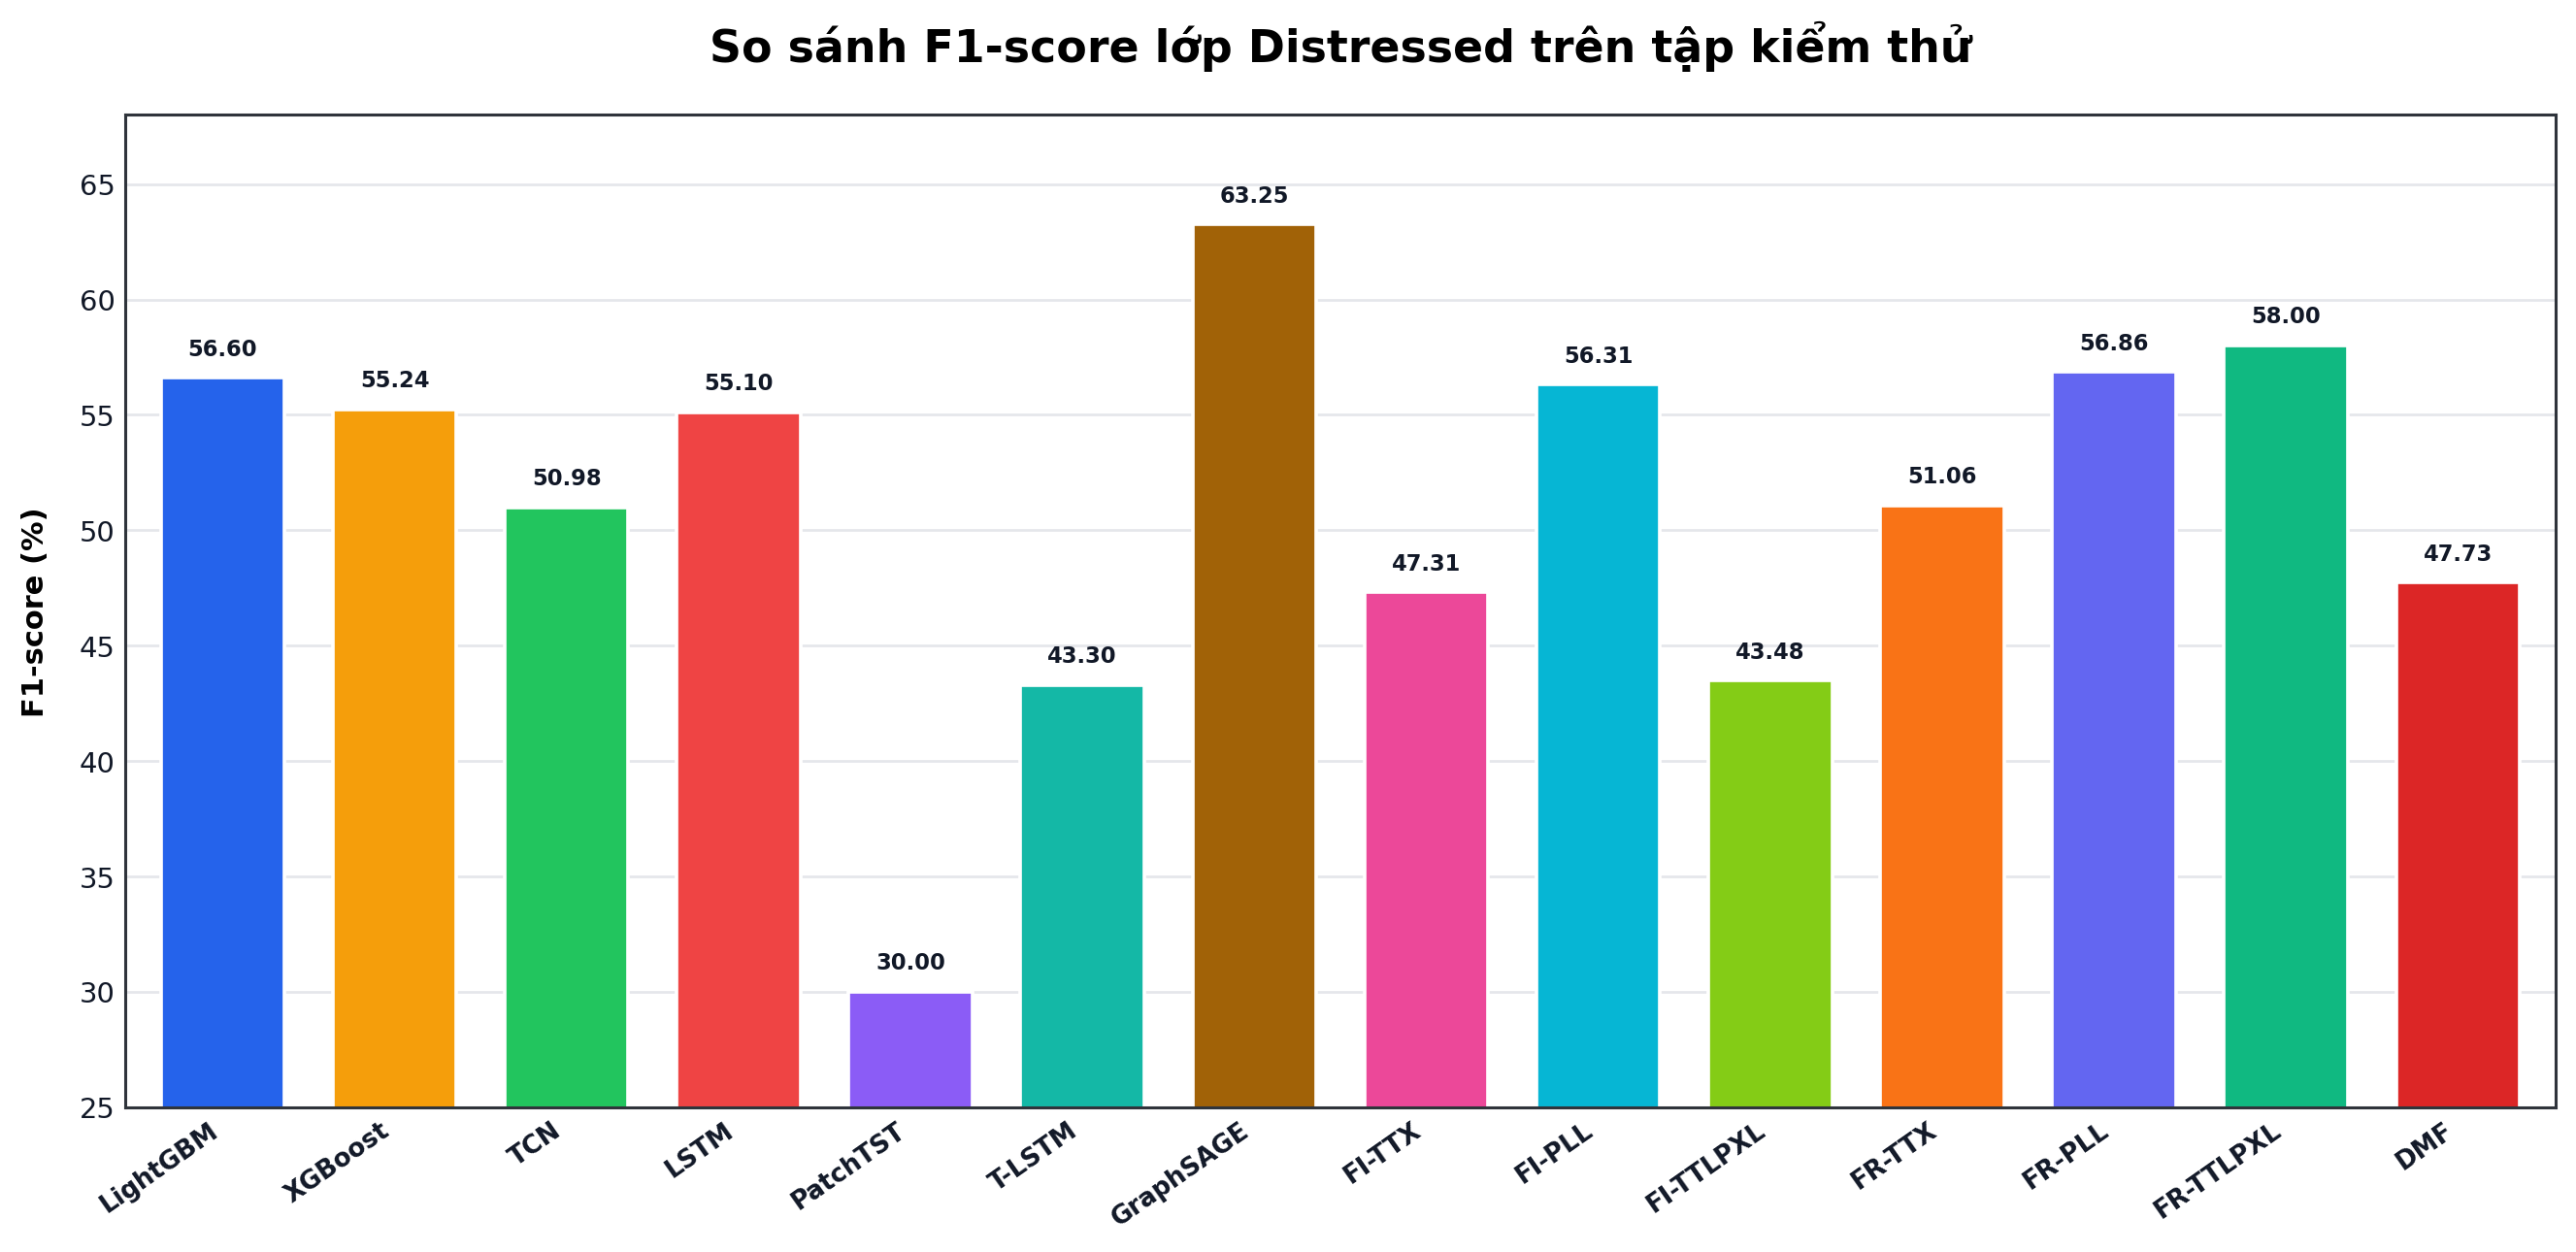
\includegraphics[width=\textwidth]{acc-loss/distressed_f1_score_test_comparison.png}
    \caption{F1-score của lớp Distressed}
    \label{fig:F1-Score_distressed}
\end{subfigure}

\vspace{0.15cm}

\begin{subfigure}{0.92\textwidth}
    \centering
    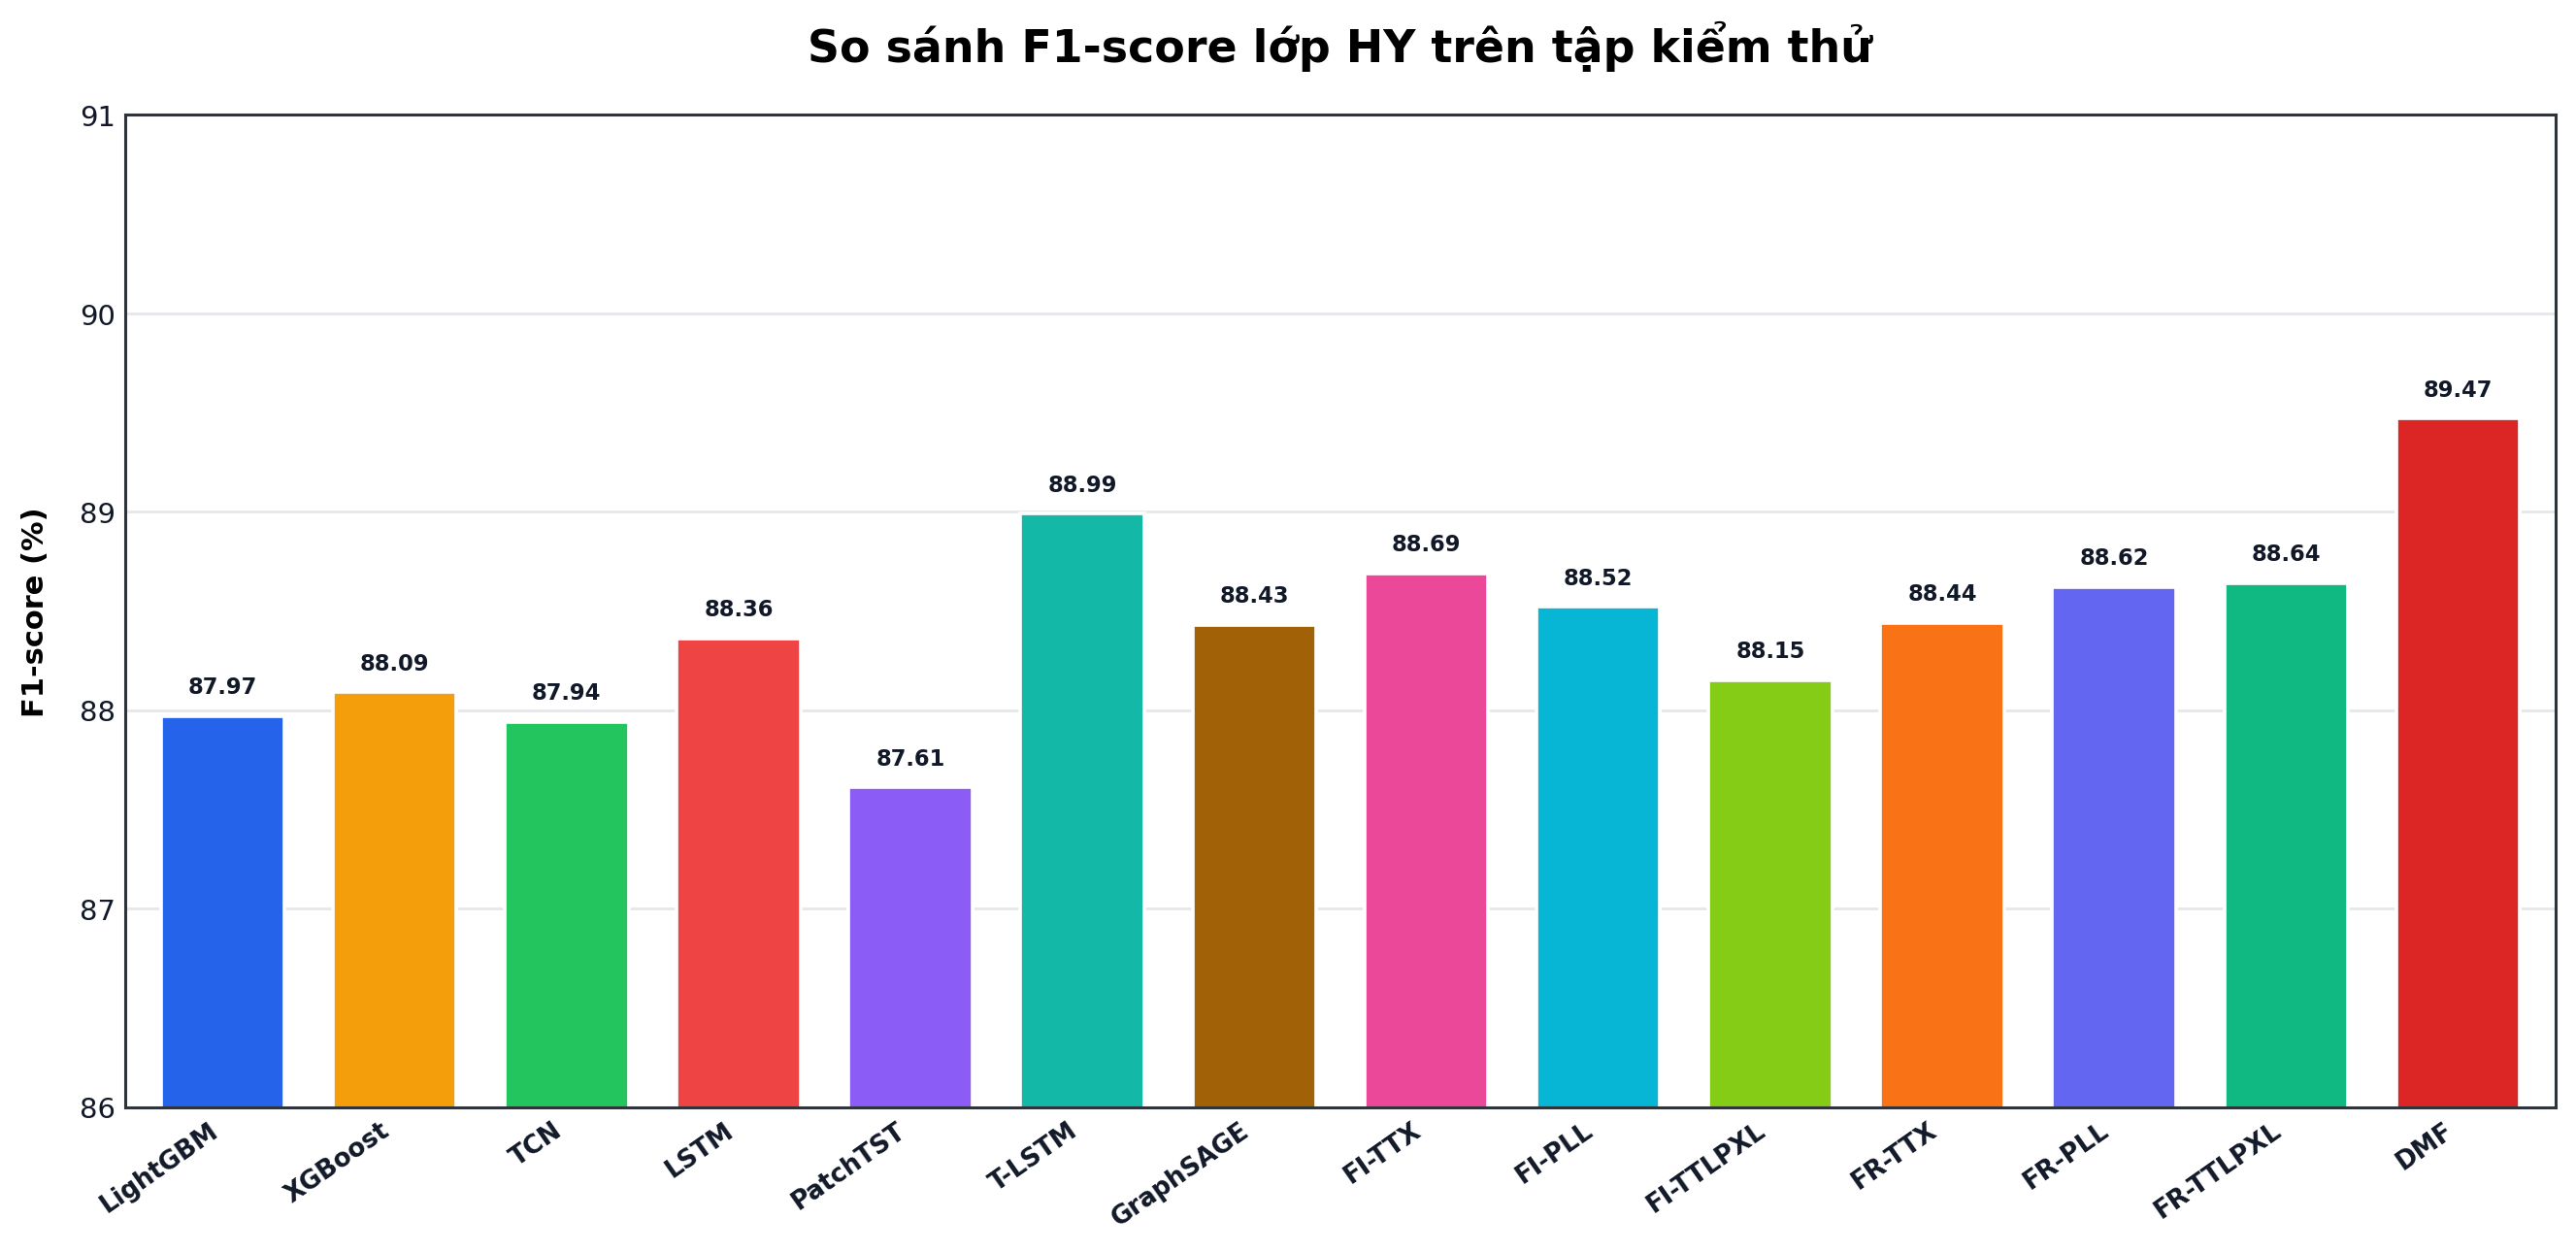
\includegraphics[width=\textwidth]{acc-loss/hy_f1_score_test_comparison.png}
    \caption{F1-score của lớp HY (High Yield)}
    \label{fig:F1-Score_hy}
\end{subfigure}

\vspace{0.15cm}

\begin{subfigure}{0.92\textwidth}
    \centering
    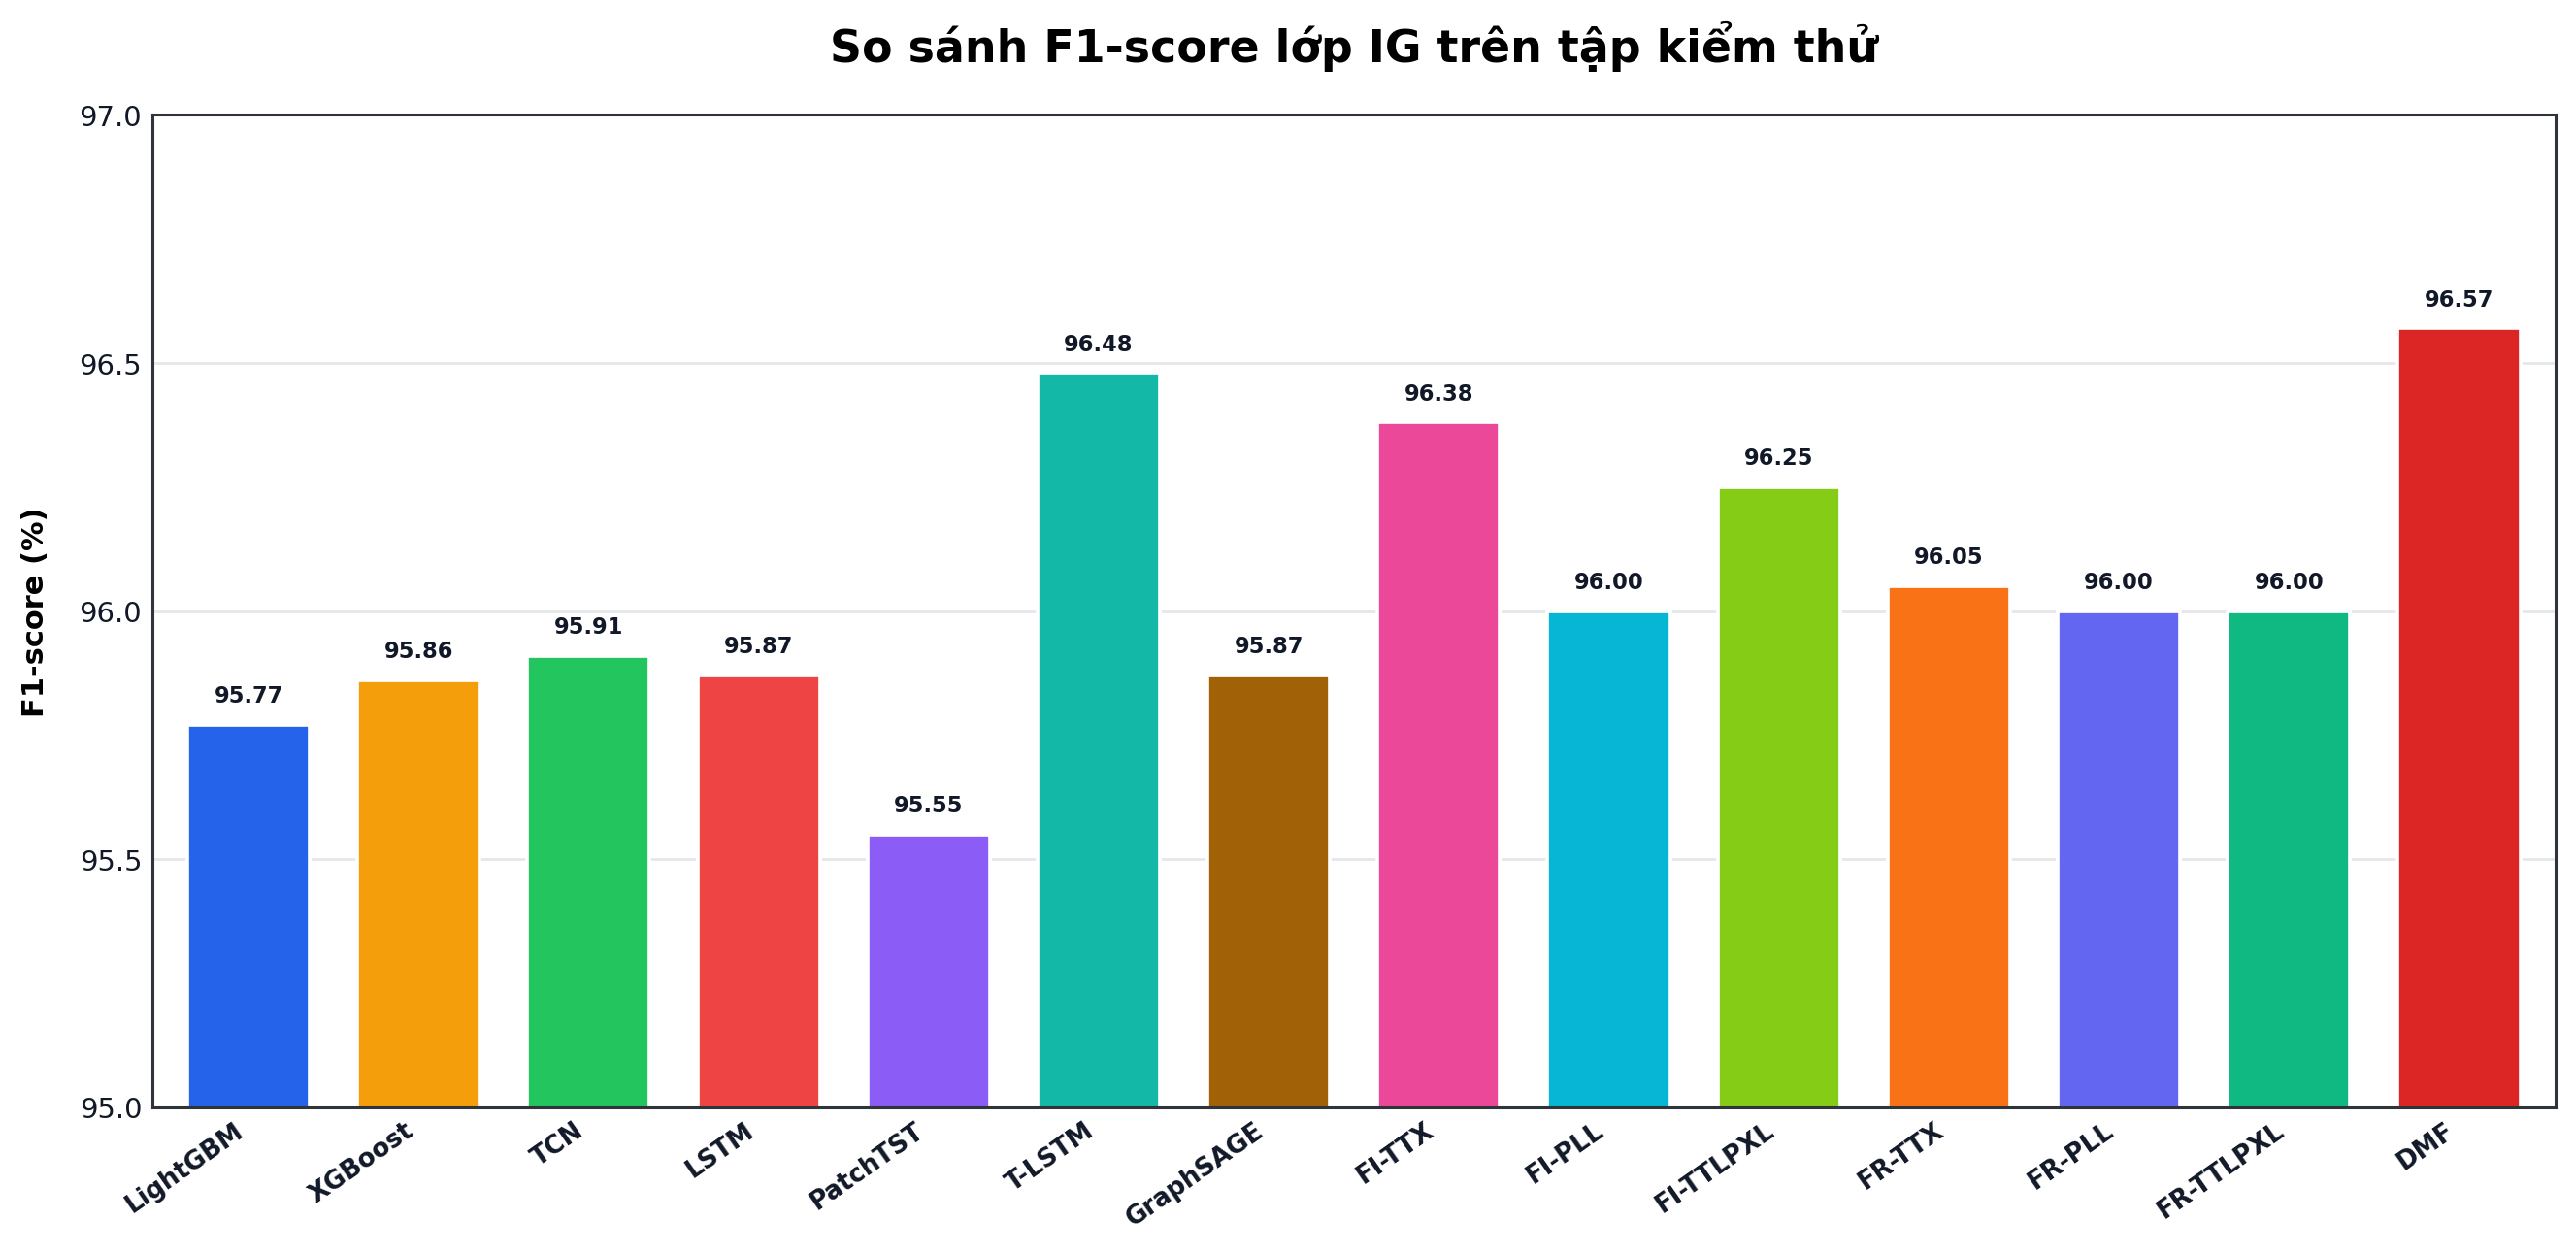
\includegraphics[width=\textwidth]{acc-loss/ig_f1_score_test_comparison.png}
    \caption{F1-score của lớp IG (Investment Grade)}
    \label{fig:F1-Score_ig}
\end{subfigure}
\label{fig:F1-Score_classes}

\caption{F1-score lớp Distressed (a), lớp HY (b) và lớp IG (c) trên tập kiểm thử}
\end{figure}
F1-score của lớp Distressed phân hóa rõ giữa các mô hình. GraphSAGE đạt giá trị cao nhất (63,25\%), FR-TTLPXL đạt 58,00\%, còn PatchTST đạt 30,00\%. Với lớp HY, F1-score nằm trong khoảng 87,61\%--89,47\%; DMF đạt mức cao nhất, tiếp theo là T-LSTM với 88,99\%. Đối với lớp IG, các mô hình đạt từ 95,55\% đến 96,57\%, trong đó DMF đạt giá trị cao nhất. Vì vậy, DMF có kết quả tốt ở hai lớp chiếm đa số, trong khi GraphSAGE phù hợp hơn khi ưu tiên nhận diện lớp Distressed.

\subsubsection{Ma trận nhầm lẫn}

\begin{table}[!htbp]
\centering
\caption{Ma trận nhầm lẫn các kịch bản trên tập kiểm thử}
\label{tab:confusion_matrices}

\renewcommand{\arraystretch}{1.2}
\setlength{\tabcolsep}{4pt}

\begin{tabular}{|>{\centering\arraybackslash}m{0.31\textwidth}|
                >{\centering\arraybackslash}m{0.31\textwidth}|
                >{\centering\arraybackslash}m{0.31\textwidth}|}
\hline

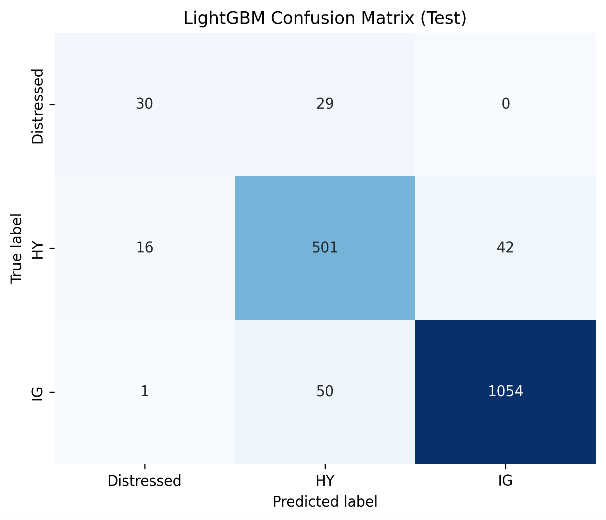
\includegraphics[width=1.00\linewidth]{acc-loss/cm-lightgbm.png} &
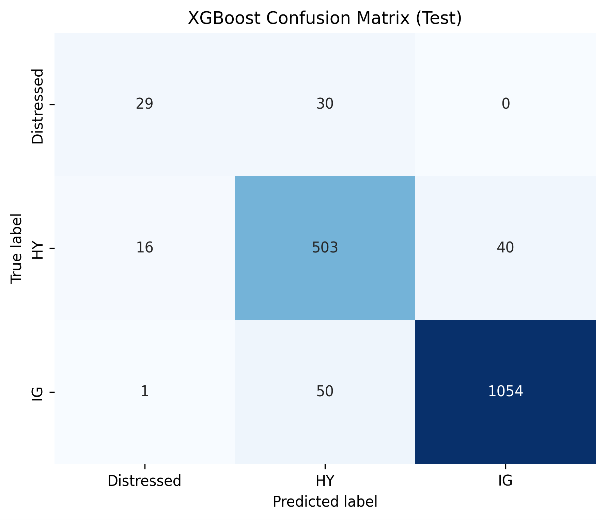
\includegraphics[width=1.00\linewidth]{acc-loss/cm-xgboost.png} &
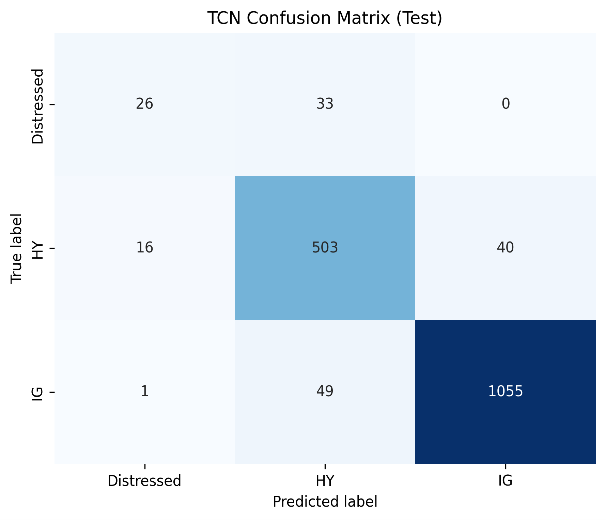
\includegraphics[width=1.00\linewidth]{acc-loss/cm-tcn.png} \\
\hline

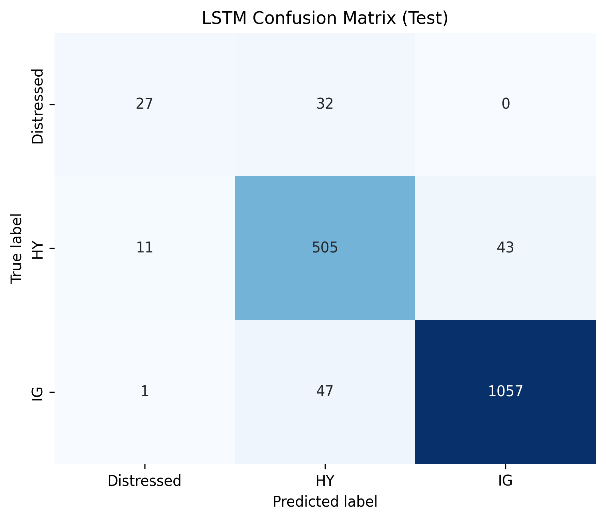
\includegraphics[width=1.00\linewidth]{acc-loss/cm-lstm.png} &
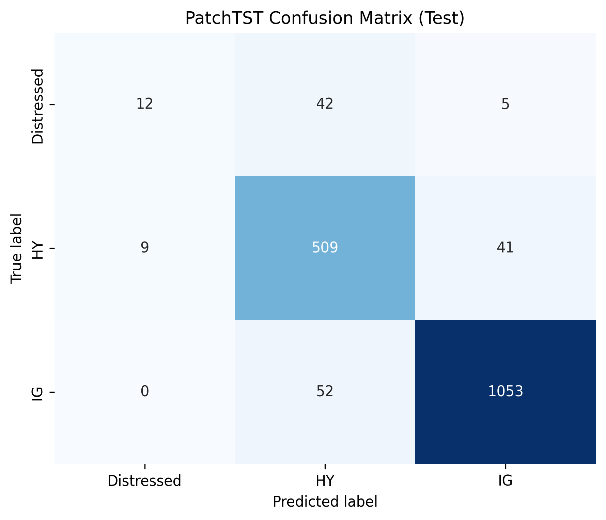
\includegraphics[width=1.00\linewidth]{acc-loss/cm-patchtst.png} &
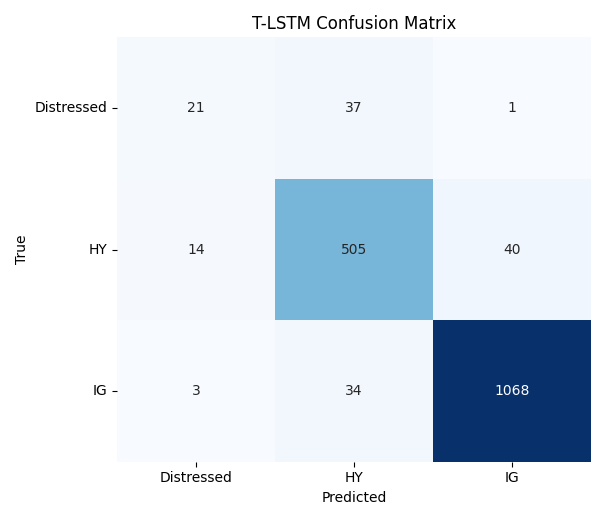
\includegraphics[width=1.00\linewidth]{acc-loss/cm-tlstm.png} \\
\hline

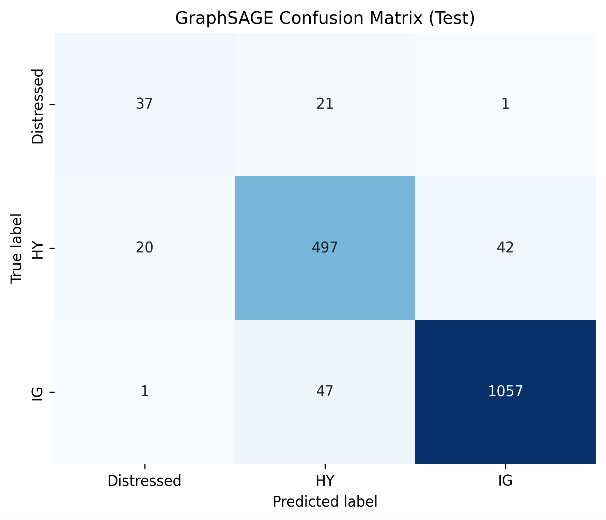
\includegraphics[width=1.00\linewidth]{acc-loss/cm-graph.png} & 
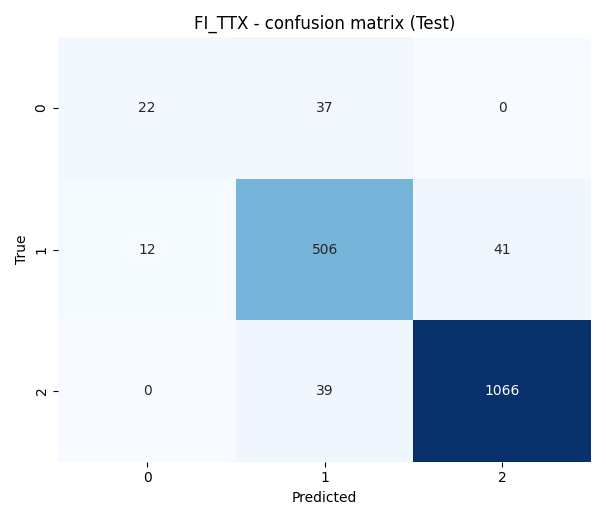
\includegraphics[width=1.00\linewidth]{acc-loss/cm-fittx.png} &
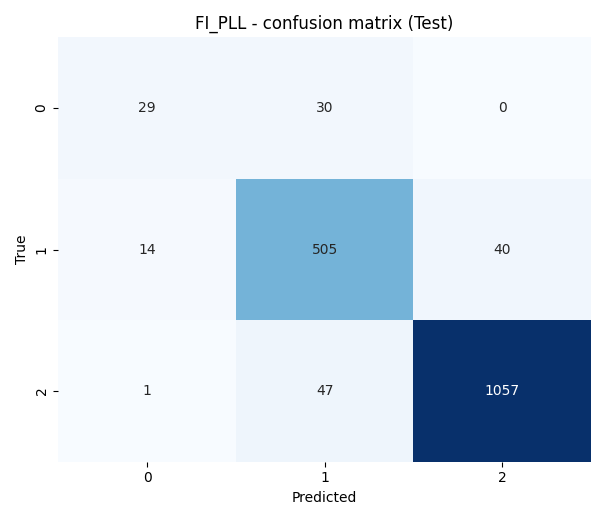
\includegraphics[width=1.00\linewidth]{acc-loss/cm-fipll.png} \\
\hline

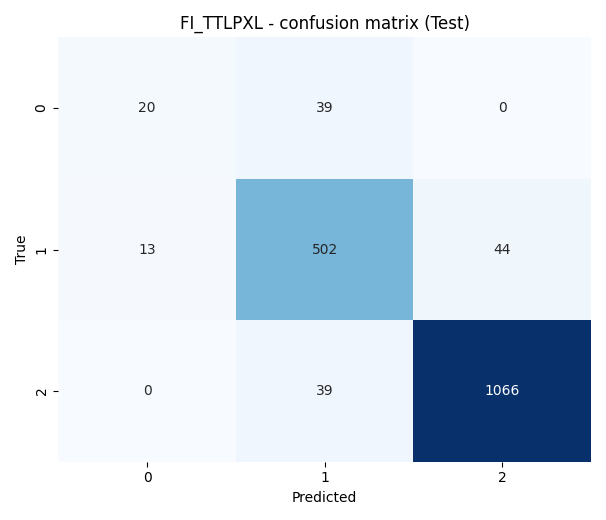
\includegraphics[width=1.00\linewidth]{acc-loss/cm-fittlpxl.png} & 
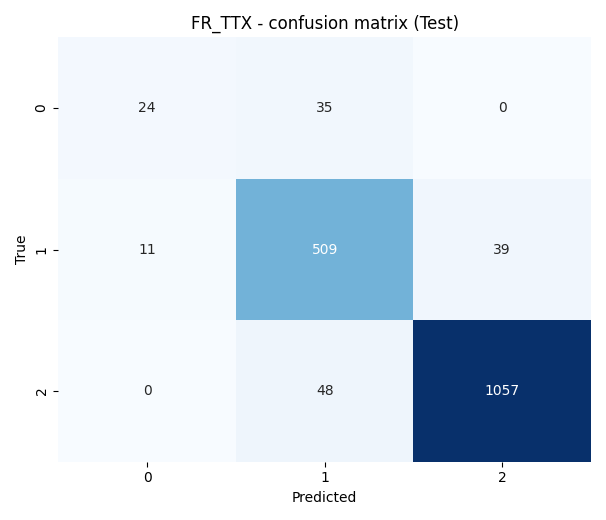
\includegraphics[width=1.00\linewidth]{acc-loss/cm-frttx.png} &
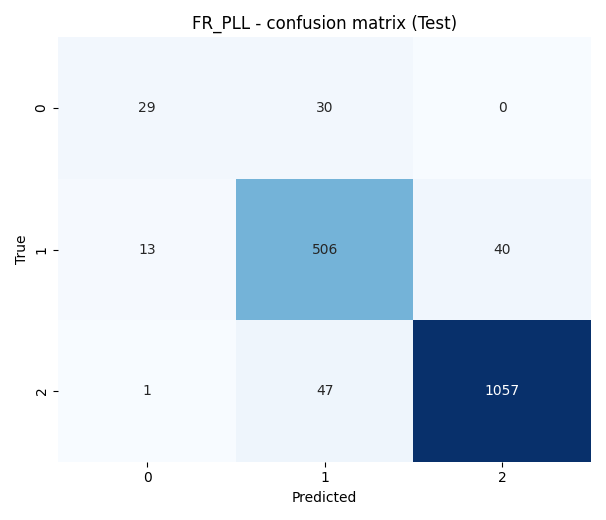
\includegraphics[width=1.00\linewidth]{acc-loss/cm-frpll.png} \\
\hline

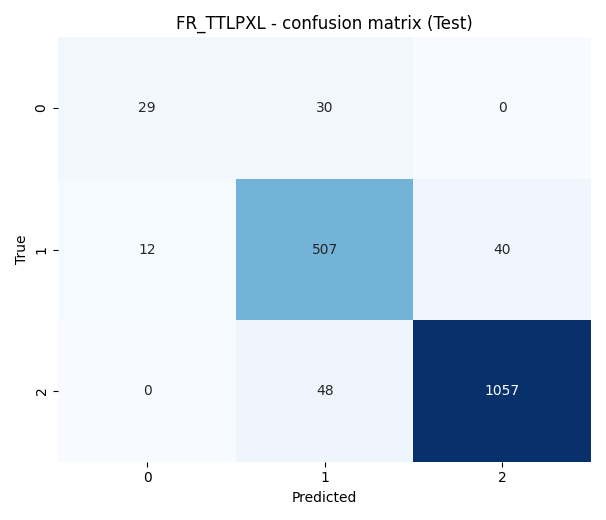
\includegraphics[width=1.00\linewidth]{acc-loss/cm-ttlpxl.png} & & \\
\hline

\end{tabular}
\end{table}

Ma trận nhầm lẫn cho thấy IG được nhận diện ổn định nhất, trong khi Distressed thường bị nhầm sang HY. GraphSAGE dự đoán đúng 37 mẫu Distressed, nhiều nhất trong nhóm mô hình riêng lẻ. T-LSTM dự đoán đúng 1.068 mẫu IG. DMF/DCS dự đoán đúng 510 mẫu HY và 1.071 mẫu IG, nhưng nhận diện Distressed kém hơn GraphSAGE. Kết quả này nhất quán với Recall theo lớp và cho thấy sự đánh đổi giữa hiệu quả tổng thể với khả năng phát hiện nhóm rủi ro cao.

\subsubsection{AUC-ROC của các kịch bản}


\begin{figure}[!htbp]
\centering


\captionsetup[subfigure]{
    labelformat=simple,
    labelsep=period,
    font=it,
    justification=centering
}

\renewcommand{\thesubfigure}{\alph{subfigure}}

\begin{subfigure}{0.78\textwidth}
    \centering
    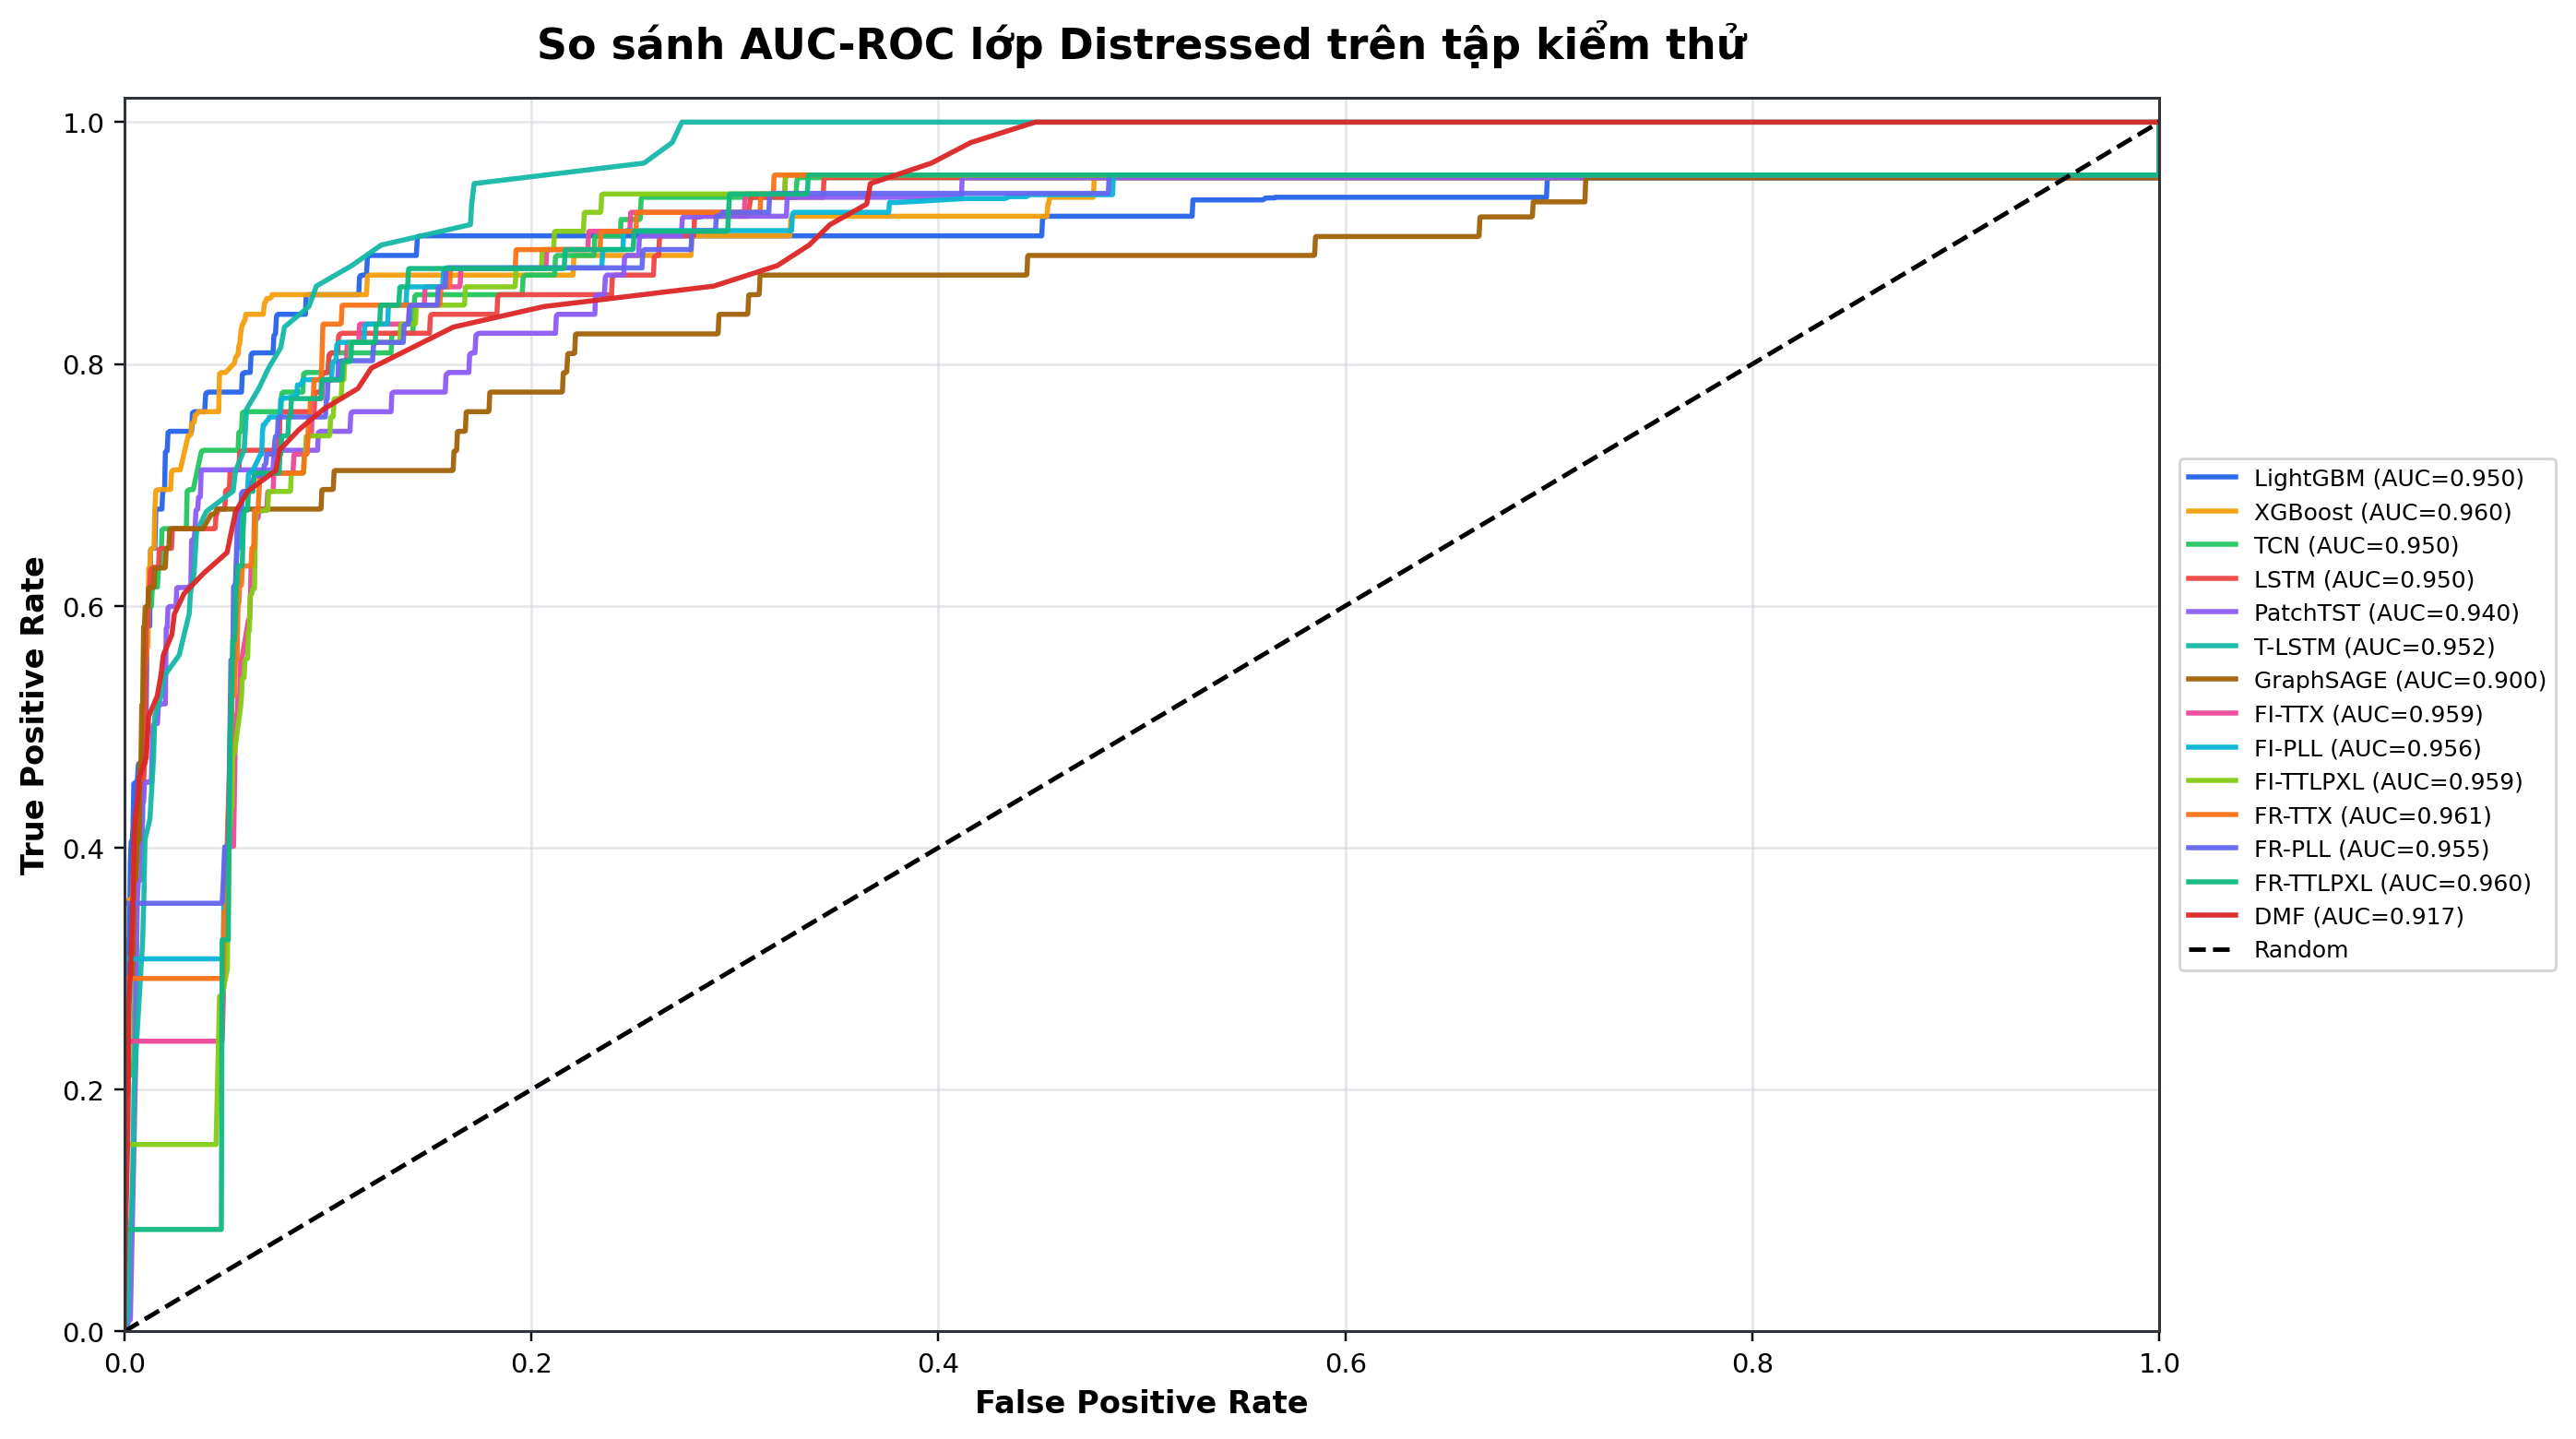
\includegraphics[width=\textwidth]{acc-loss/combined_auc_roc_distressed_14_models.png}
    \caption{Đường cong ROC trên lớp Distressed}
    \label{fig:AUC-ROC_distressed}
\end{subfigure}

\vspace{0.15cm}

\begin{subfigure}{0.78\textwidth}
    \centering
    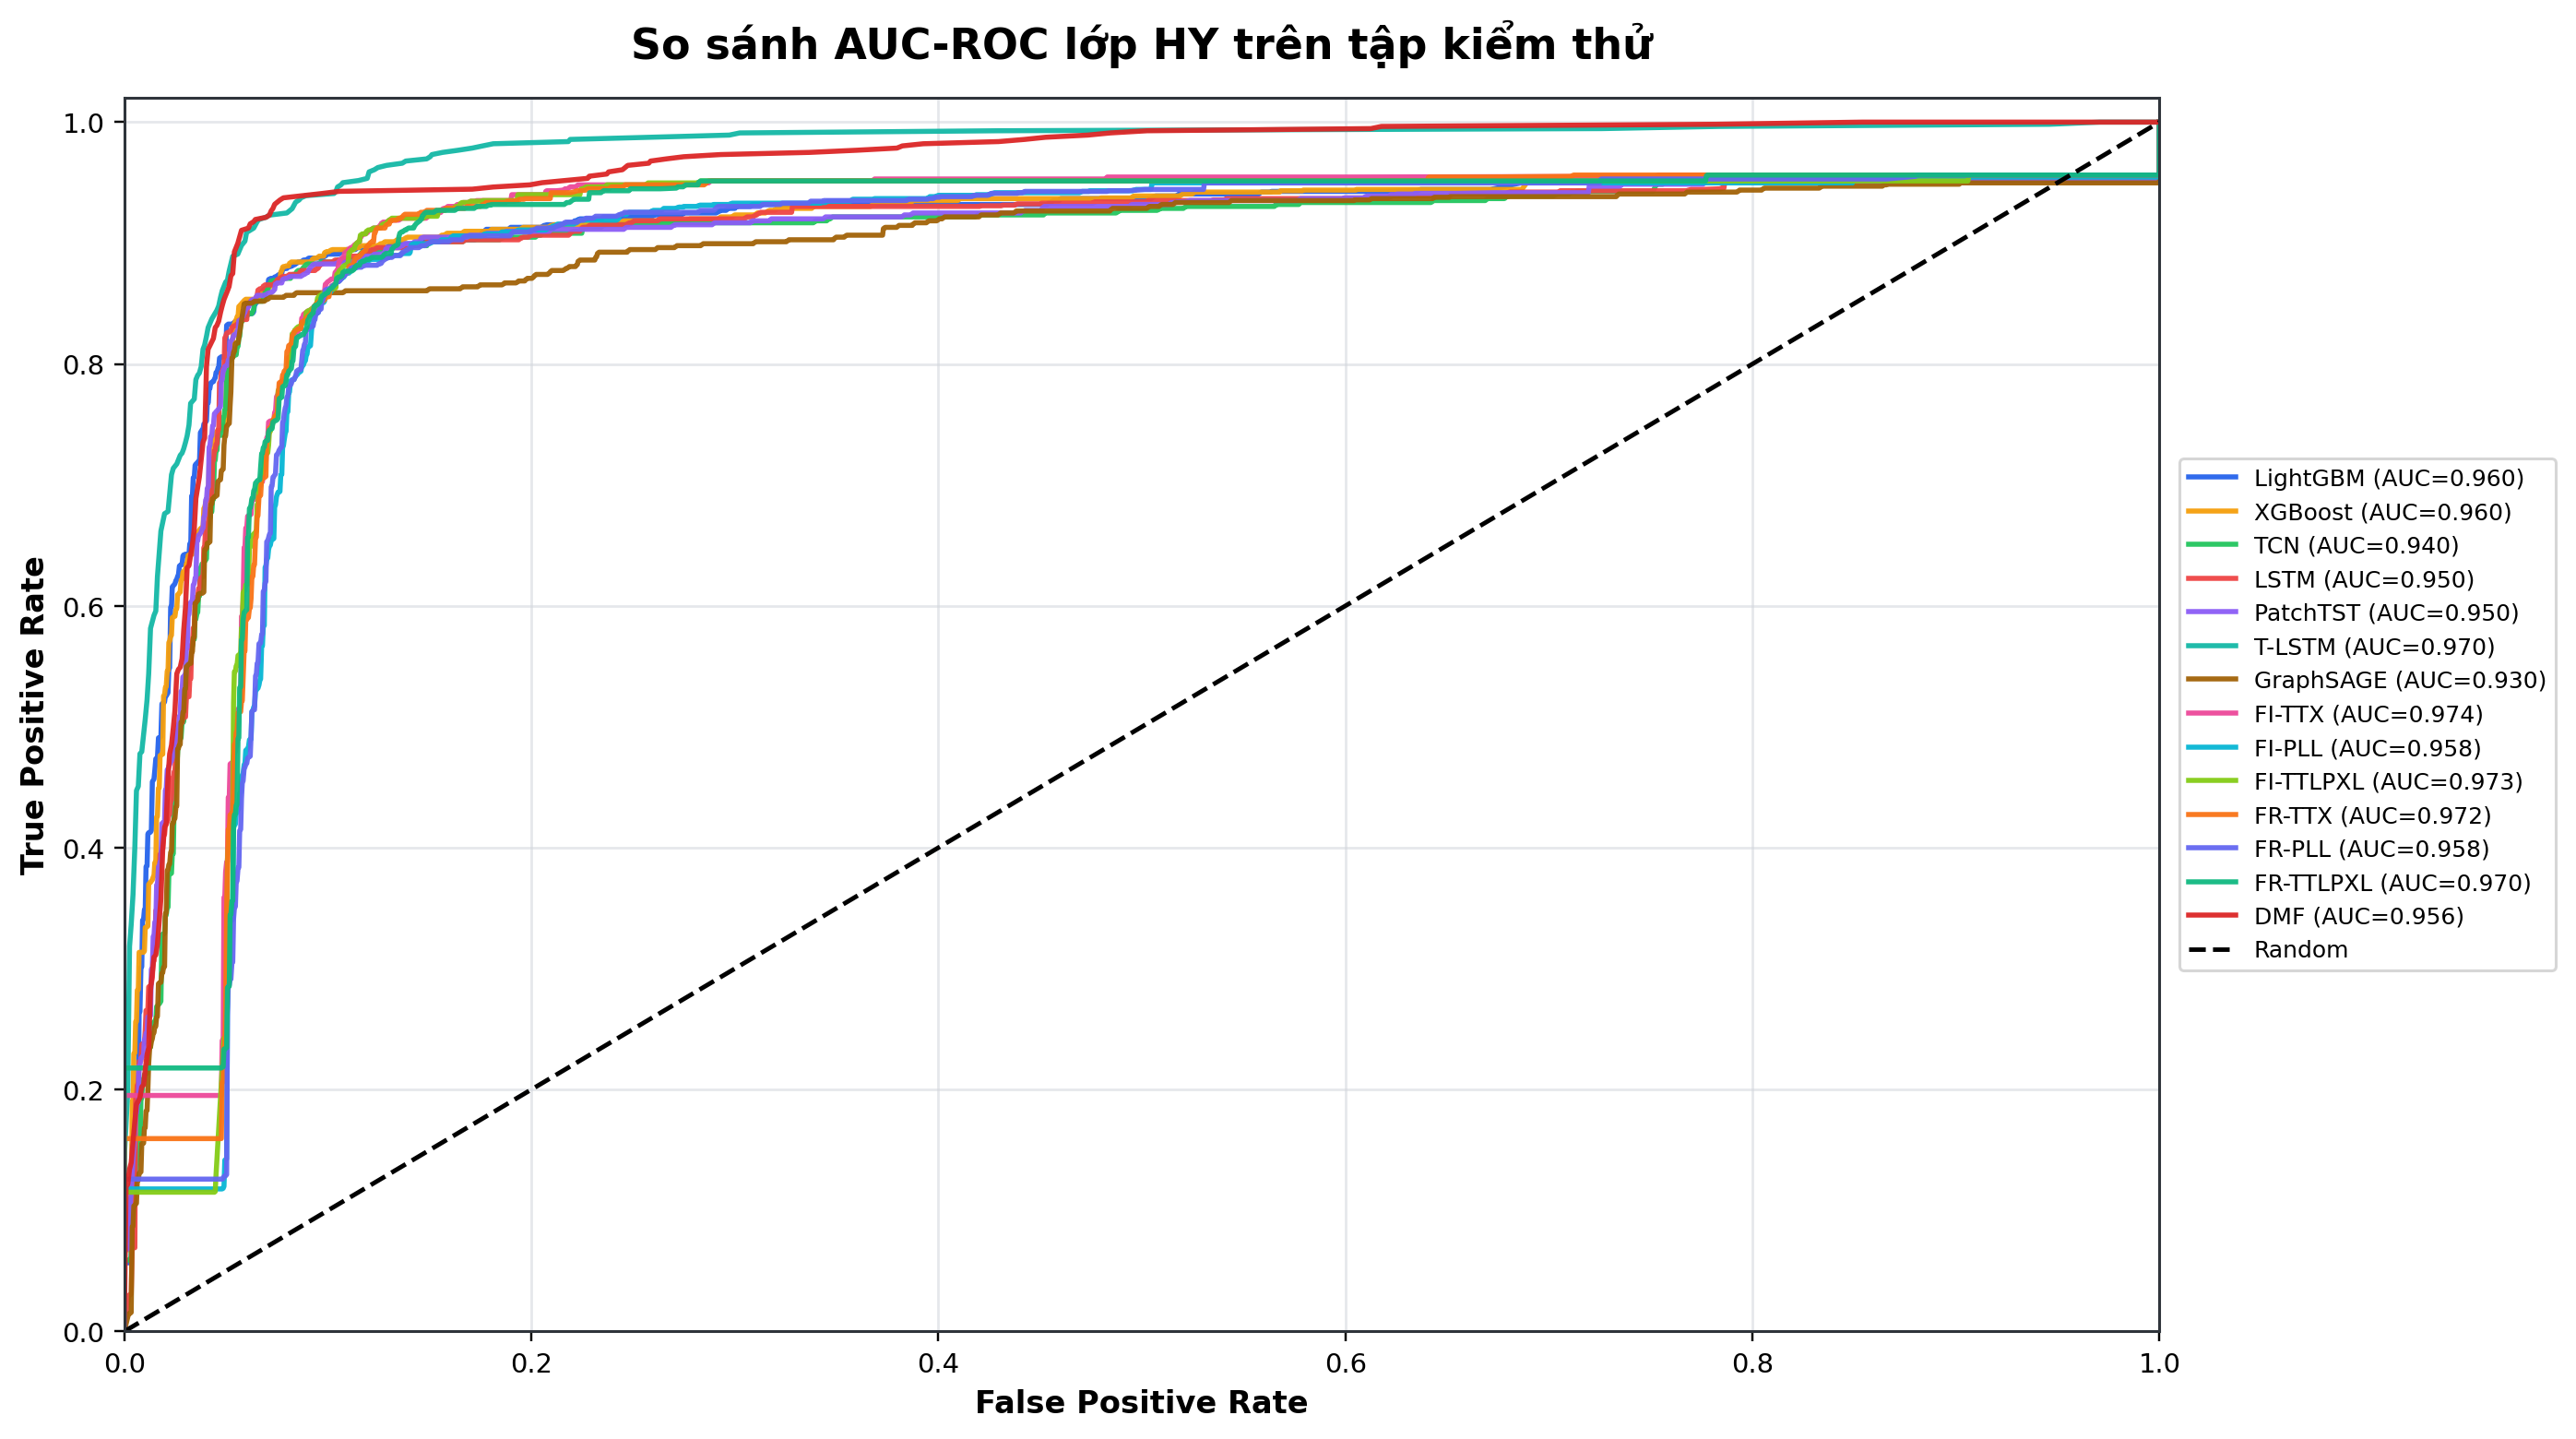
\includegraphics[width=\textwidth]{acc-loss/combined_auc_roc_hy_14_models.png}
    \caption{Đường cong ROC trên lớp HY (High Yield)}
    \label{fig:AUC-ROC_hy}
\end{subfigure}

\vspace{0.15cm}

\begin{subfigure}{0.78\textwidth}
    \centering
    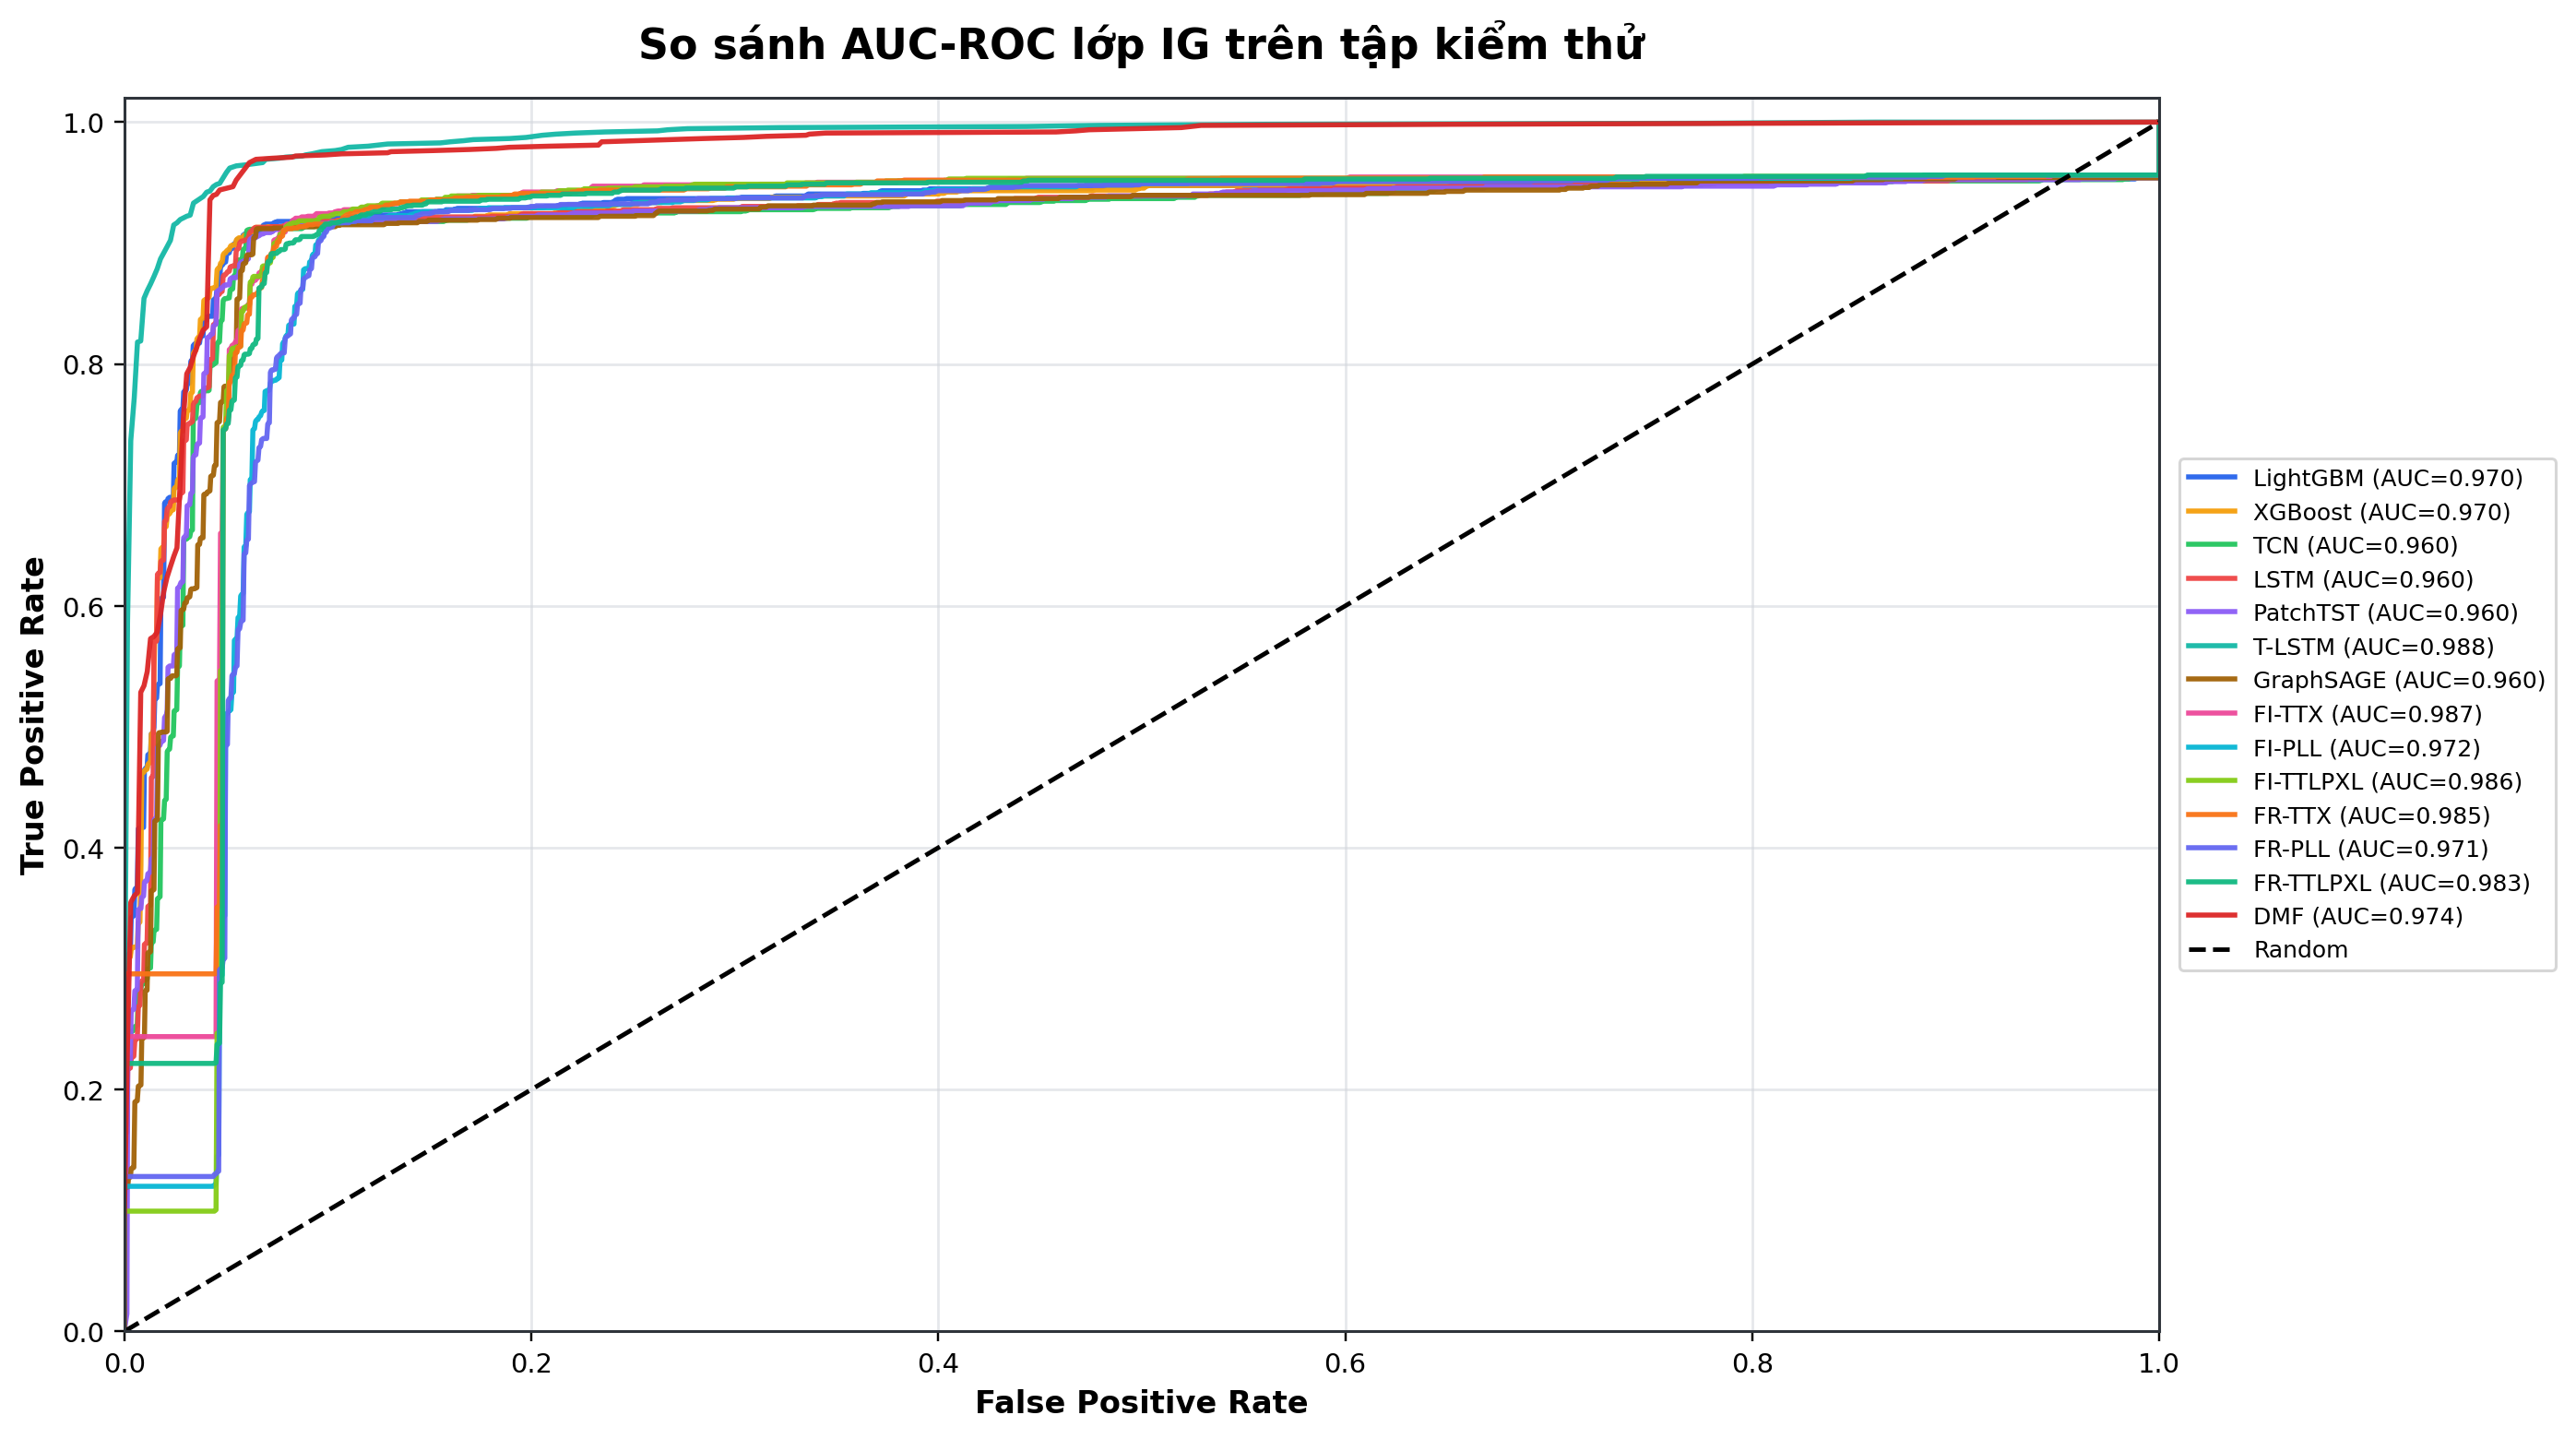
\includegraphics[width=\textwidth]{acc-loss/combined_auc_roc_ig_14_models.png}
    \caption{Đường cong ROC trên lớp IG (Investment Grade)}
    \label{fig:AUC-ROC_ig}
\end{subfigure}
\label{fig:AUC-ROC_classes}

\caption{AUC-ROC lớp Distressed (a), lớp HY(b) và lớp IG (c) trên tập kiểm thử}
\end{figure}
AUC-ROC đạt giá trị cao ở cả ba lớp nhưng mô hình dẫn đầu thay đổi theo lớp. FR-TTX đạt AUC cao nhất cho Distressed (96,1\%); FI-TTX đạt cao nhất cho HY (97,4\%); T-LSTM đạt cao nhất cho IG (98,8\%). DMF có Accuracy tổng thể cao nhất nhưng không dẫn đầu AUC ở từng lớp. Do đó, việc lựa chọn mô hình phụ thuộc vào mục tiêu ưu tiên hiệu quả tổng thể hay khả năng phân biệt một nhóm rủi ro cụ thể.

\subsubsection{Thời gian kiểm thử}
\begin{figure}[!htbp]
    \centering % Căn giữa hình ảnh
    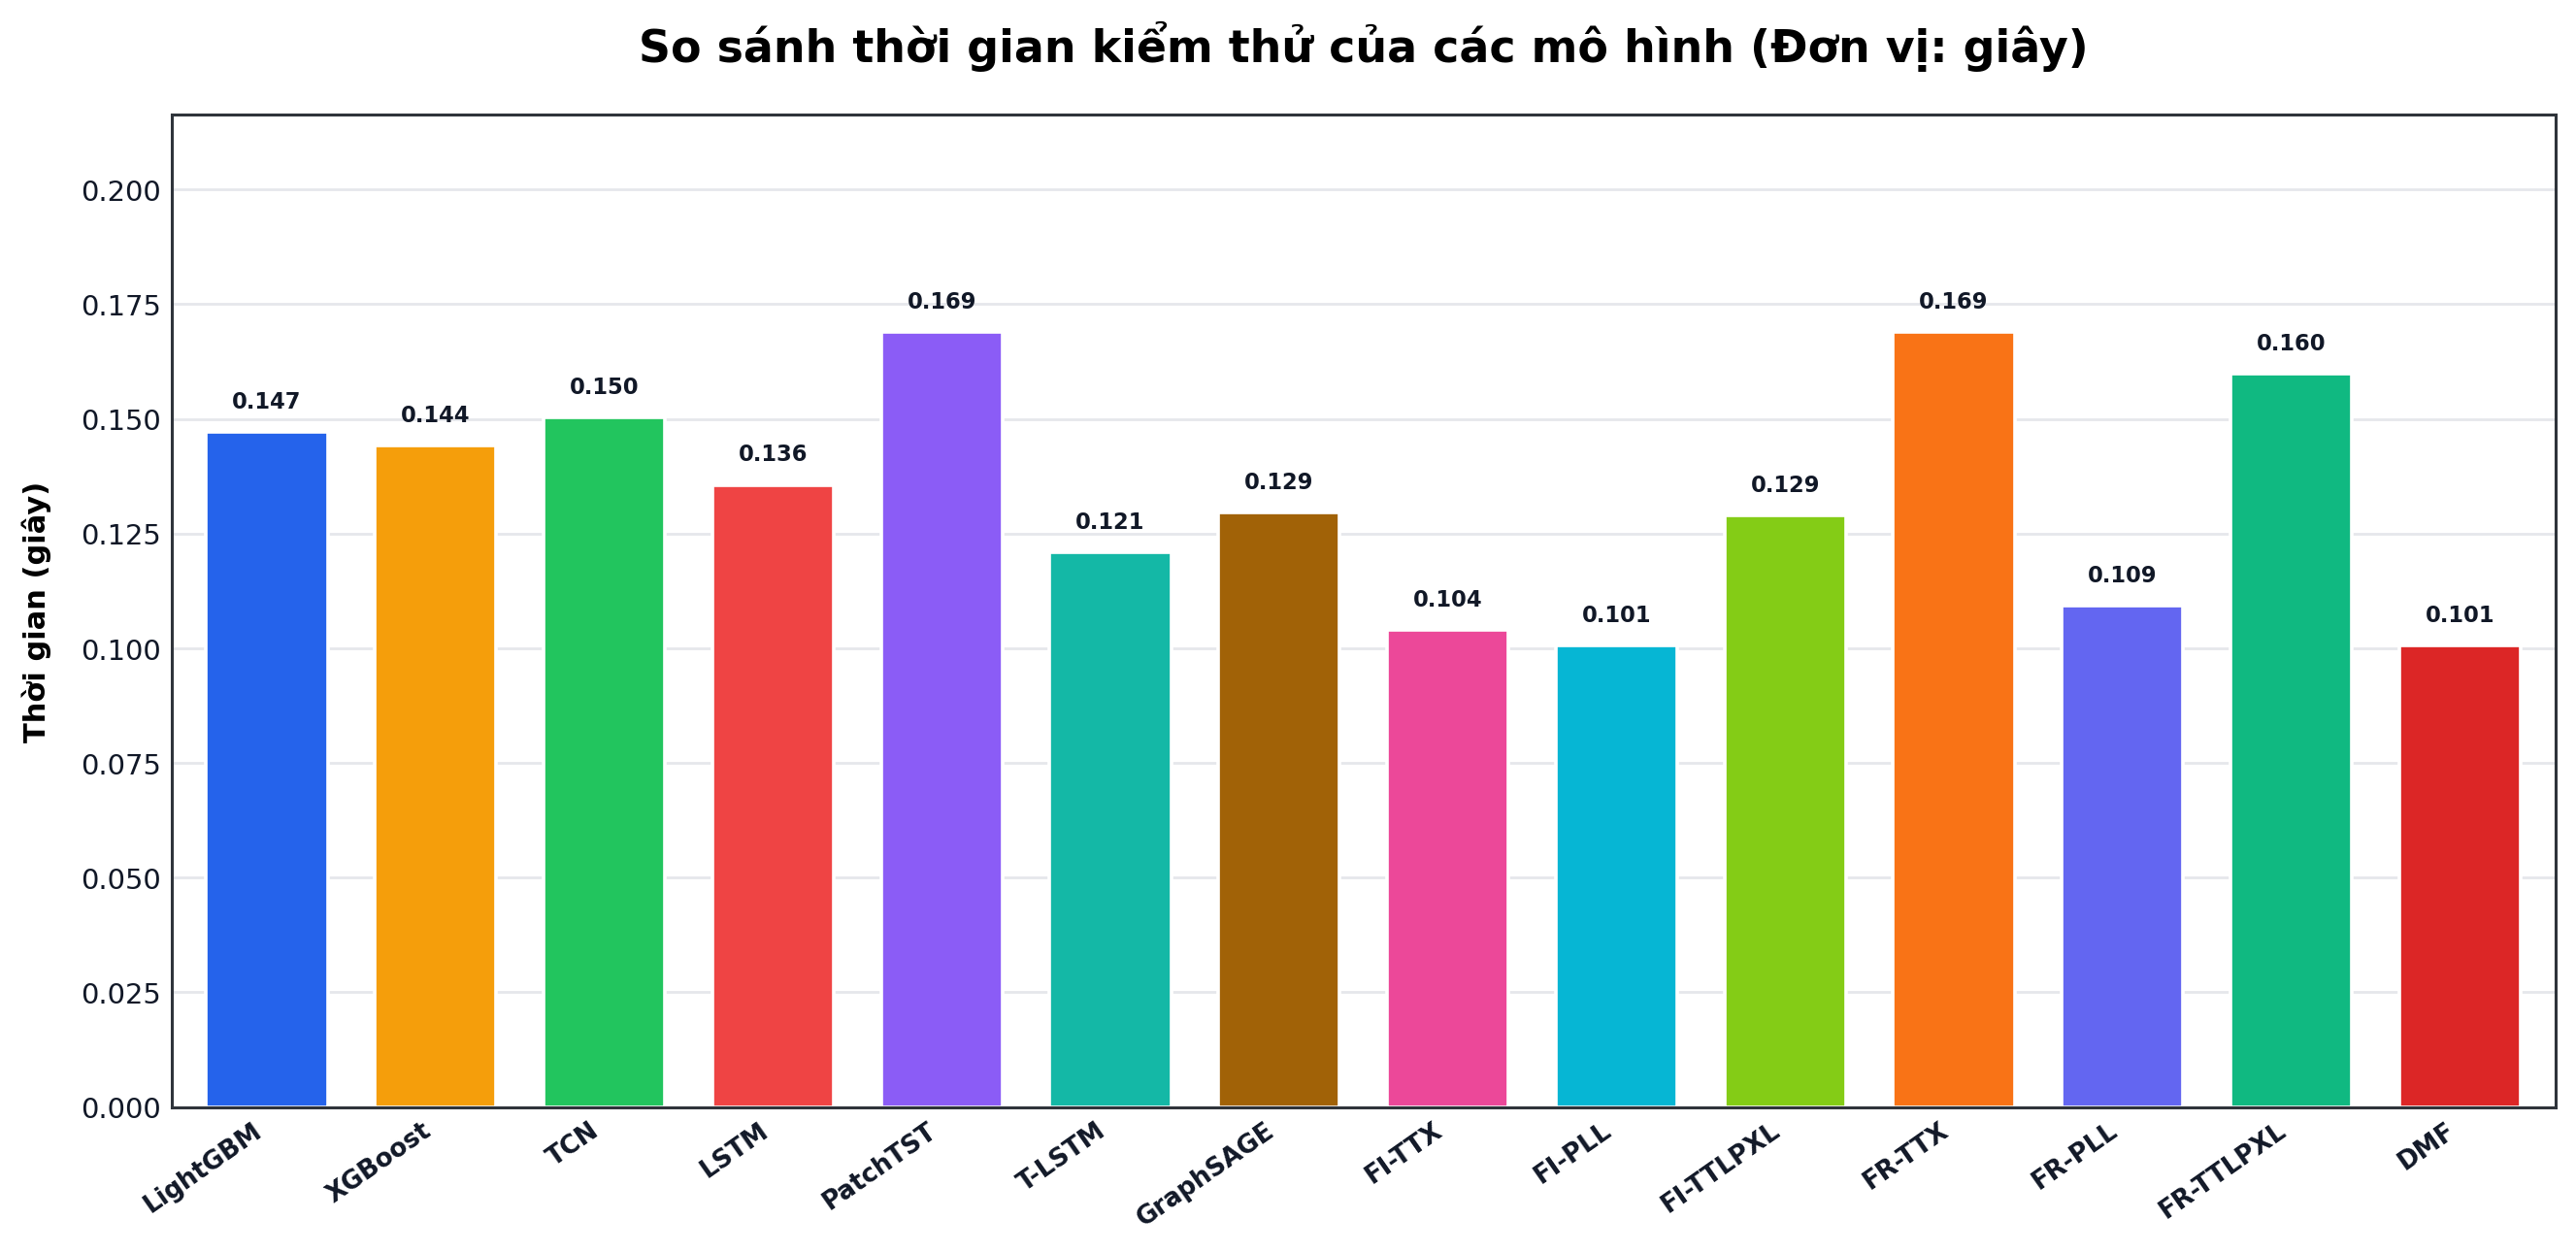
\includegraphics[width=1\textwidth]{acc-loss/test_inference_time_comparison.png} % Thay 'ten-file-anh' bằng tên ảnh của bạn (không cần đuôi .png/.jpg)
    \caption{Thời gian kiểm thử của các kịch bản} % Dòng chú thích dưới ảnh
\end{figure}

Thời gian kiểm thử dao động từ 0,101 đến 0,169 giây trong môi trường thực nghiệm. FI-PLL và DMF có thời gian thấp nhất (0,101 giây), còn PatchTST và FR-TTX có thời gian cao nhất (0,169 giây). Mức chênh lệch tuyệt đối giữa các kịch bản là 0,068 giây. Các số liệu này cho thấy chi phí suy luận thấp trên tập kiểm thử hiện tại, nhưng chưa đủ để kết luận về hiệu năng khi triển khai ở quy mô lớn hoặc trên hạ tầng khác.

\subsubsection{Kết quả giải thích bằng XAI}
\paragraph{GradientSHAP}
GradientSHAP được sử dụng để đo lường mức độ đóng góp của từng chỉ số tài chính vào xác suất dự báo của mô hình. Phương pháp này được triển khai trực tiếp trên mô hình đã huấn luyện, không sử dụng mô hình thay thế. Các đặc trưng chuỗi tài chính được rút gọn bằng giá trị trung bình theo cửa sổ thời gian, sau đó GradientSHAP ước lượng mức đóng góp của từng biến thông qua nhiều lần lấy mẫu giữa mẫu cần giải thích và tập nền.

\begin{table}[!htbp] \centering \caption{Kết quả GradientSHAP của các kịch bản trên tập kiểm thử} \label{tab:gradientshap_results} \renewcommand{\arraystretch}{0.85} \setlength{\tabcolsep}{2pt} \begin{tabular}{|>{\centering\arraybackslash}m{0.47\textwidth}| >{\centering\arraybackslash}m{0.47\textwidth}|} \hline \textbf{Kết quả GradientSHAP của kịch bản 1} & \textbf{Kết quả GradientSHAP của kịch bản 2} \\ 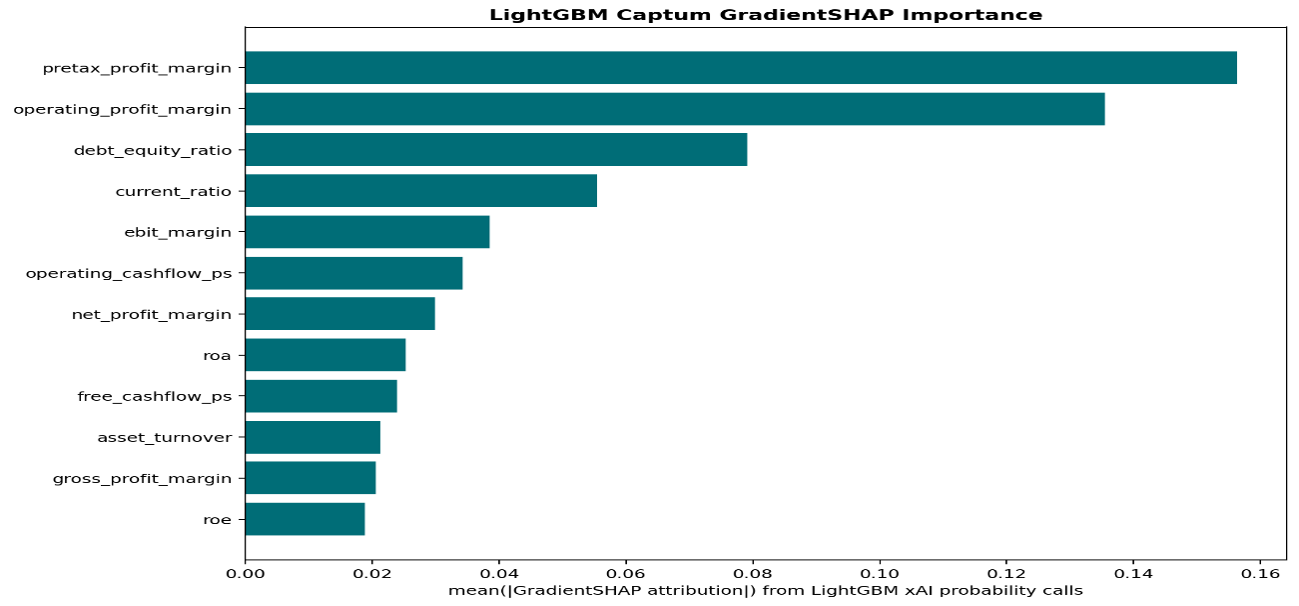
\includegraphics[width=0.55\linewidth]{acc-loss/shap-lightgbm.png} & 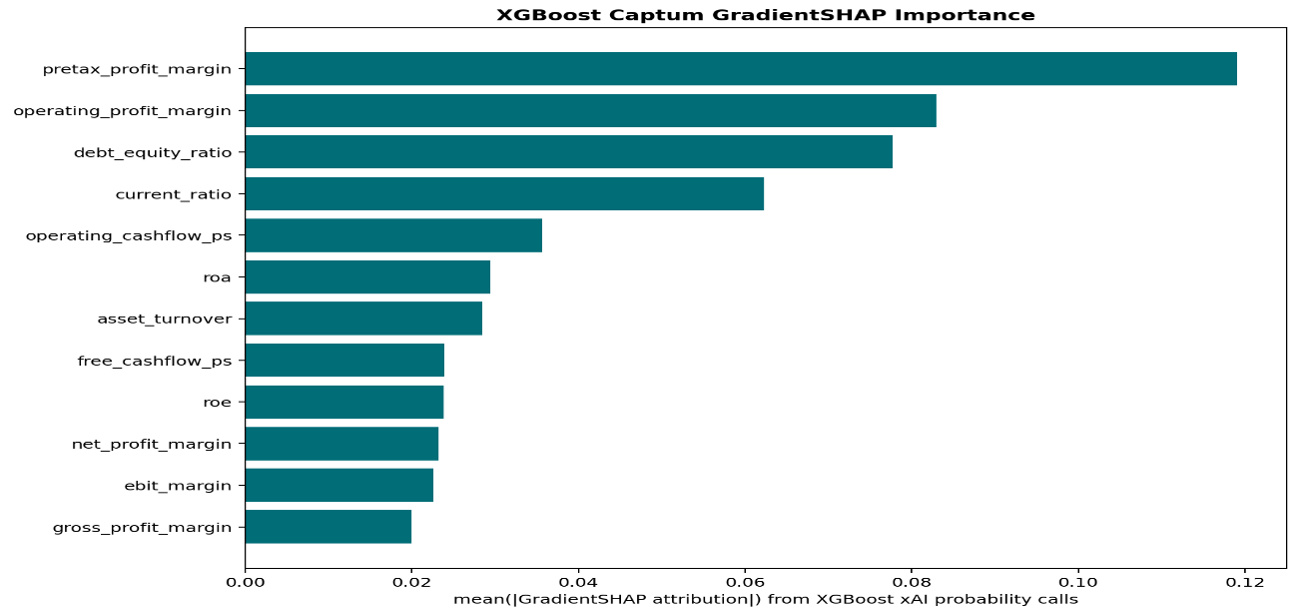
\includegraphics[width=0.55\linewidth]{acc-loss/shap-xgboost.png} \\ \hline \textbf{Kết quả GradientSHAP của kịch bản 3} & \textbf{Kết quả GradientSHAP của kịch bản 4} \\ 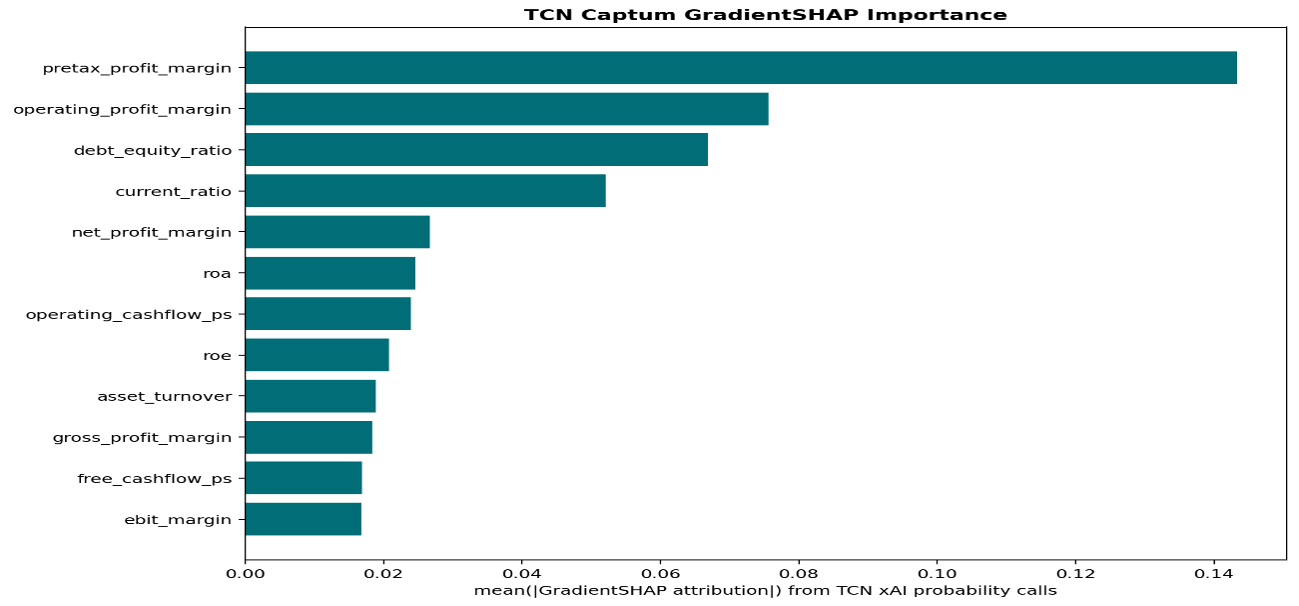
\includegraphics[width=0.55\linewidth]{acc-loss/shap-tcn.png} & 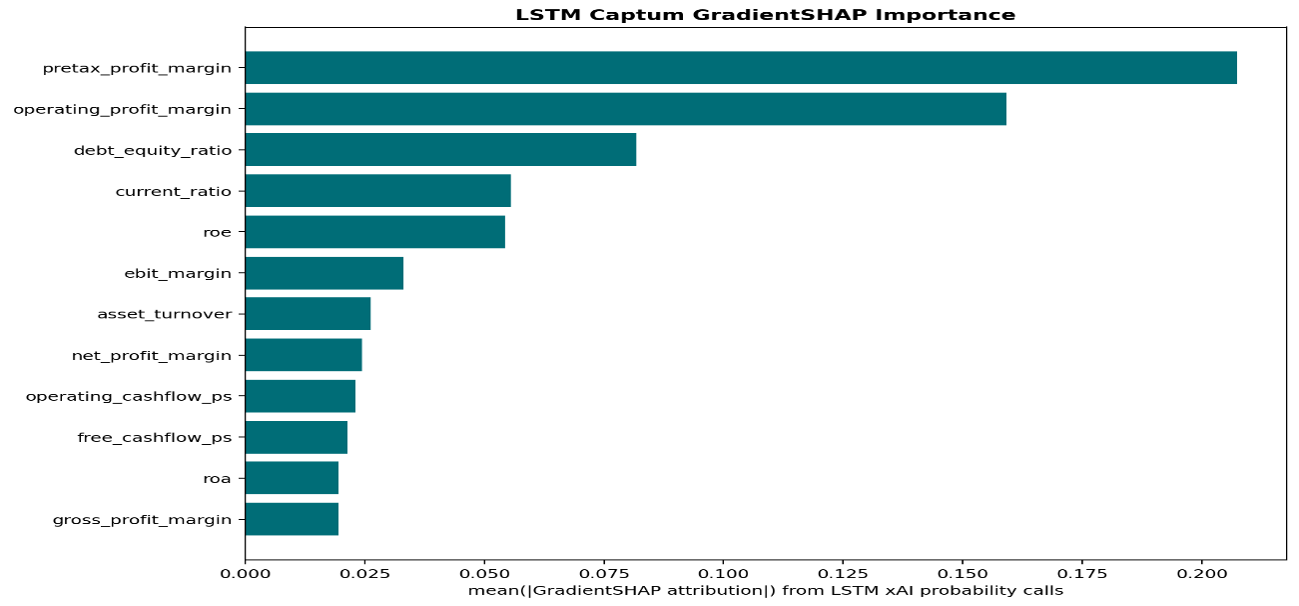
\includegraphics[width=0.55\linewidth]{acc-loss/shap-lstm.png} \\ \hline \textbf{Kết quả GradientSHAP của kịch bản 5} & \textbf{Kết quả GradientSHAP của kịch bản 6} \\ 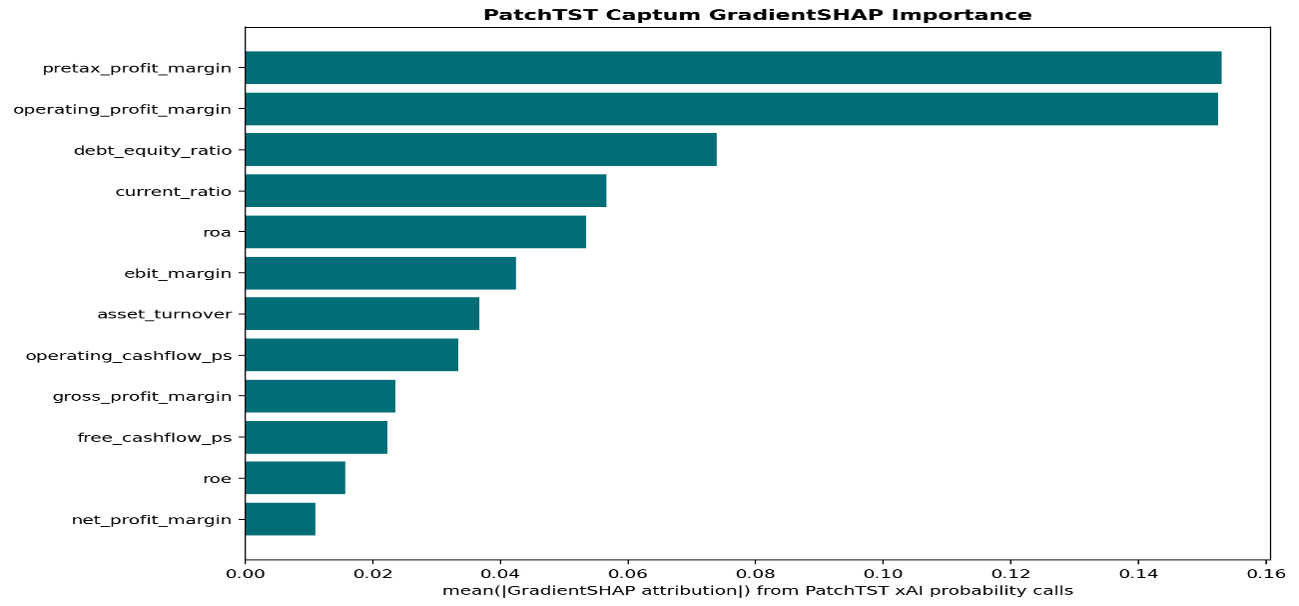
\includegraphics[width=0.55\linewidth]{acc-loss/shap-patchtst.png} & 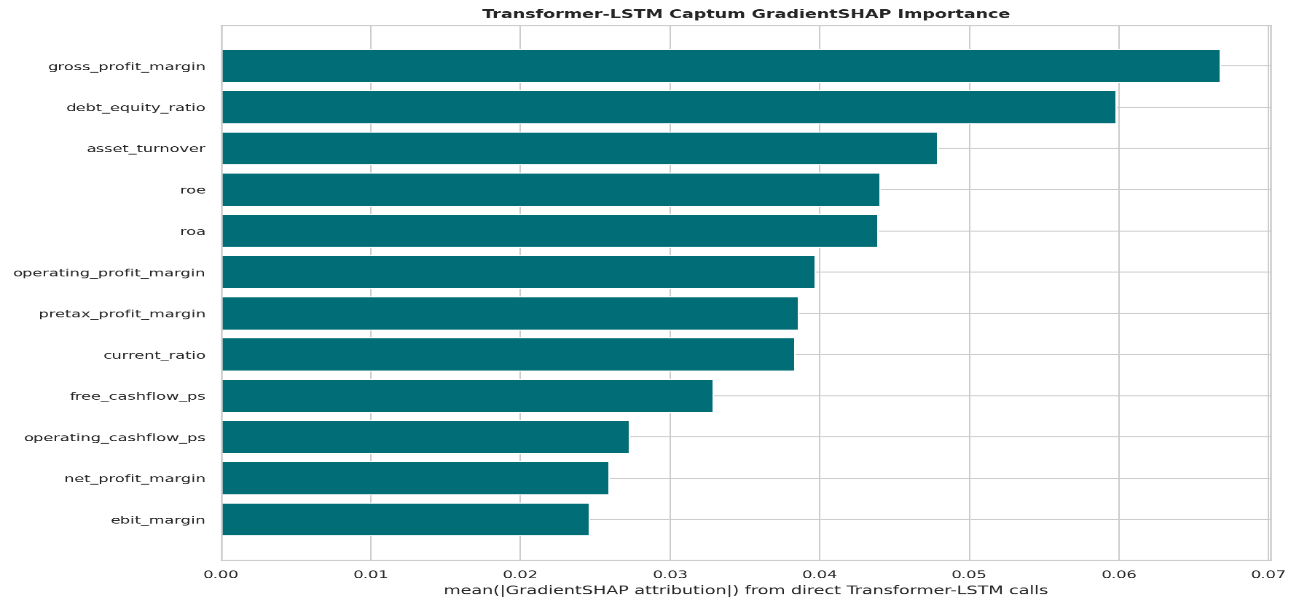
\includegraphics[width=0.55\linewidth]{acc-loss/shap-tlstm.png} \\ \hline \textbf{Kết quả GradientSHAP của kịch bản 7} & \textbf{Kết quả GradientSHAP của kịch bản 8} \\ 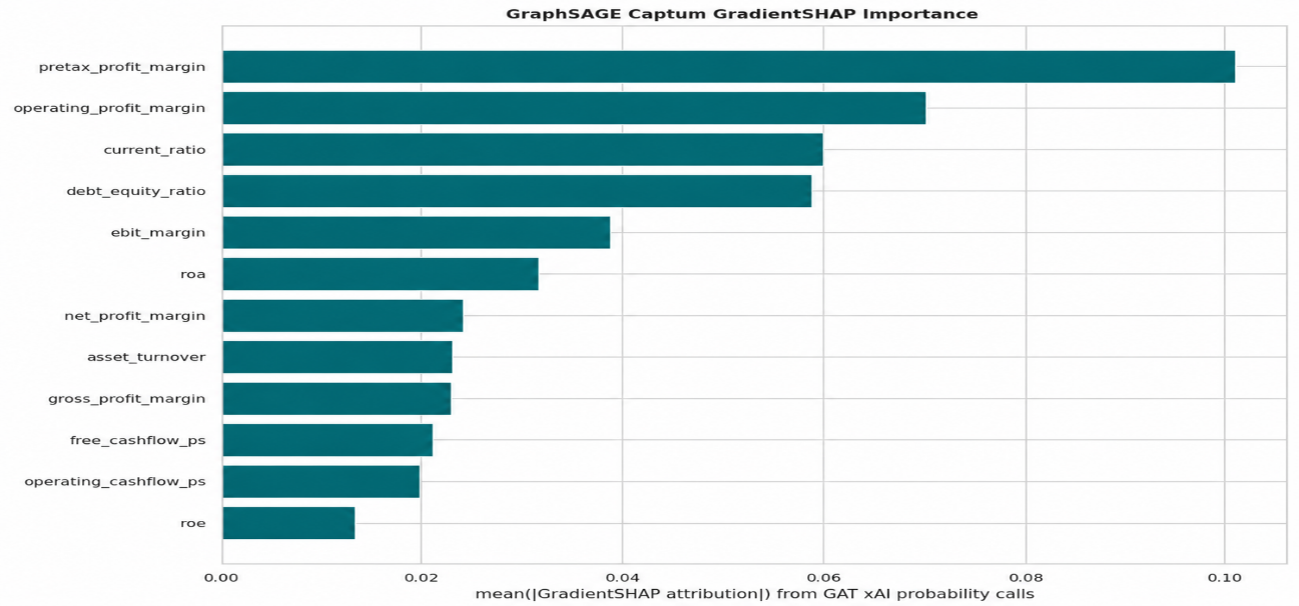
\includegraphics[width=0.55\linewidth]{acc-loss/shap-graph.png} & 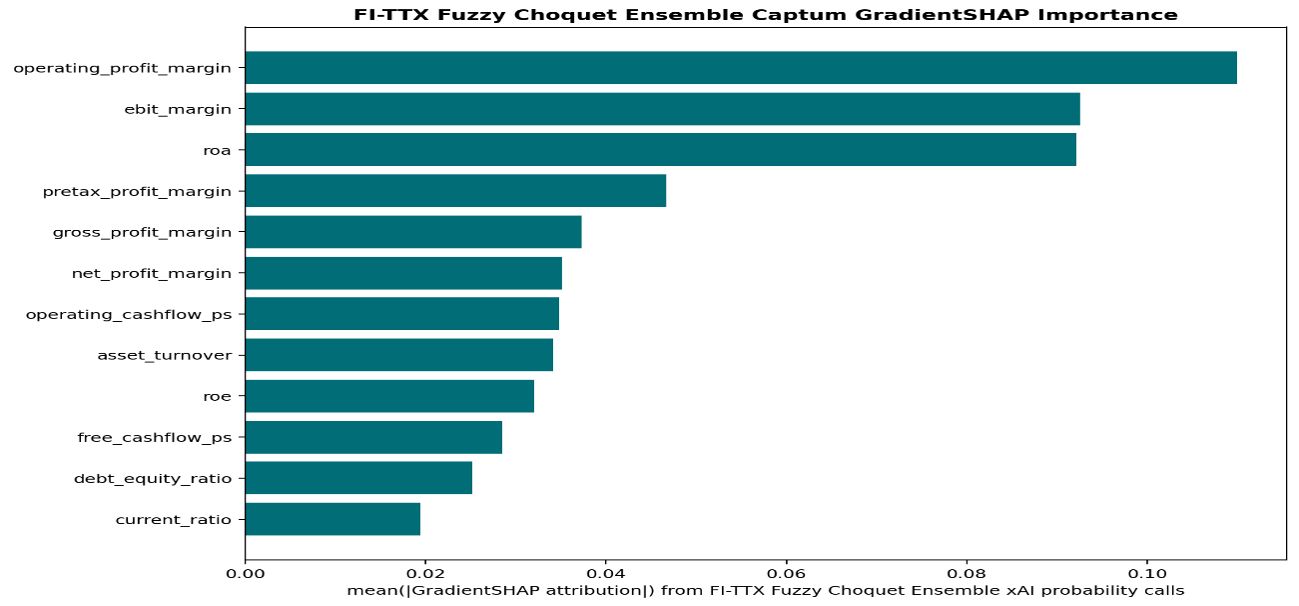
\includegraphics[width=0.55\linewidth]{acc-loss/shap-fittx.png} \\ \hline \textbf{Kết quả GradientSHAP của kịch bản 9} & \textbf{Kết quả GradientSHAP của kịch bản 10} \\ 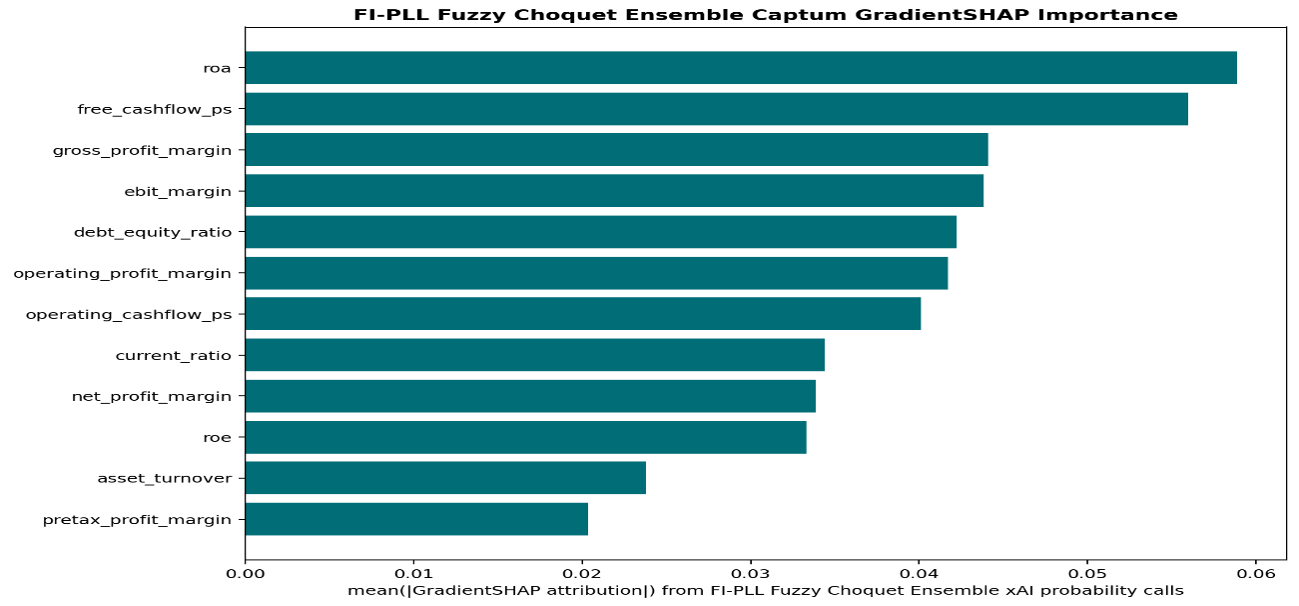
\includegraphics[width=0.55\linewidth]{acc-loss/shap-fipll.png} & 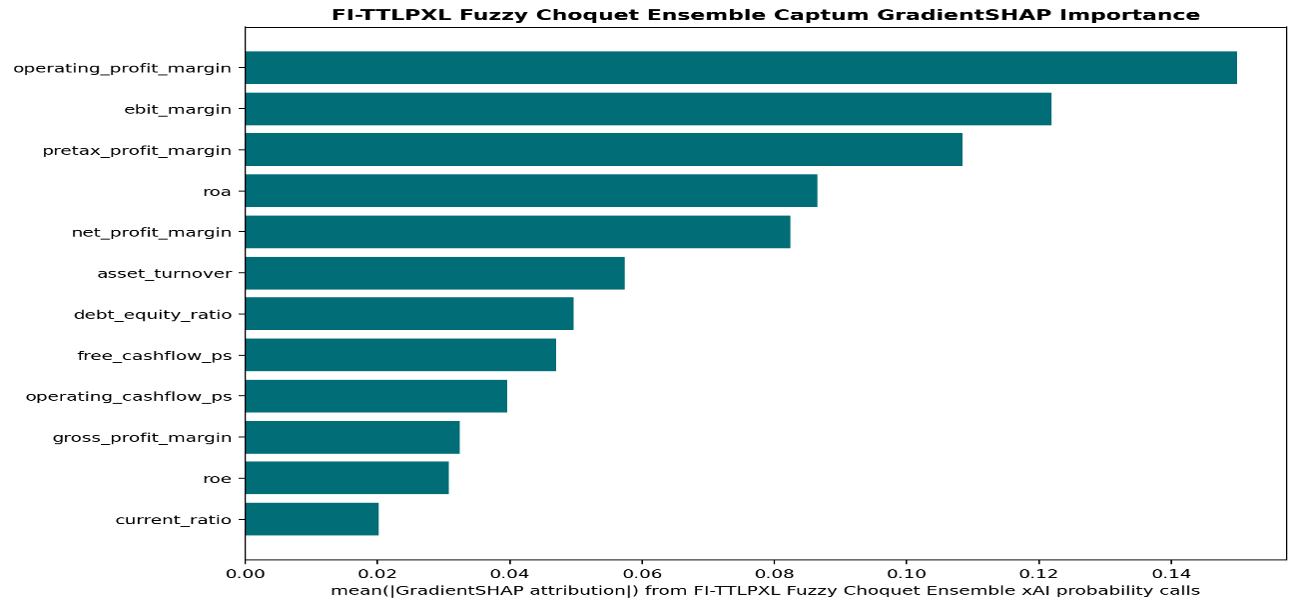
\includegraphics[width=0.55\linewidth]{acc-loss/shap-fittlpxl.png} \\ \hline \textbf{Kết quả GradientSHAP của kịch bản 11} & \textbf{Kết quả GradientSHAP của kịch bản 12} \\ 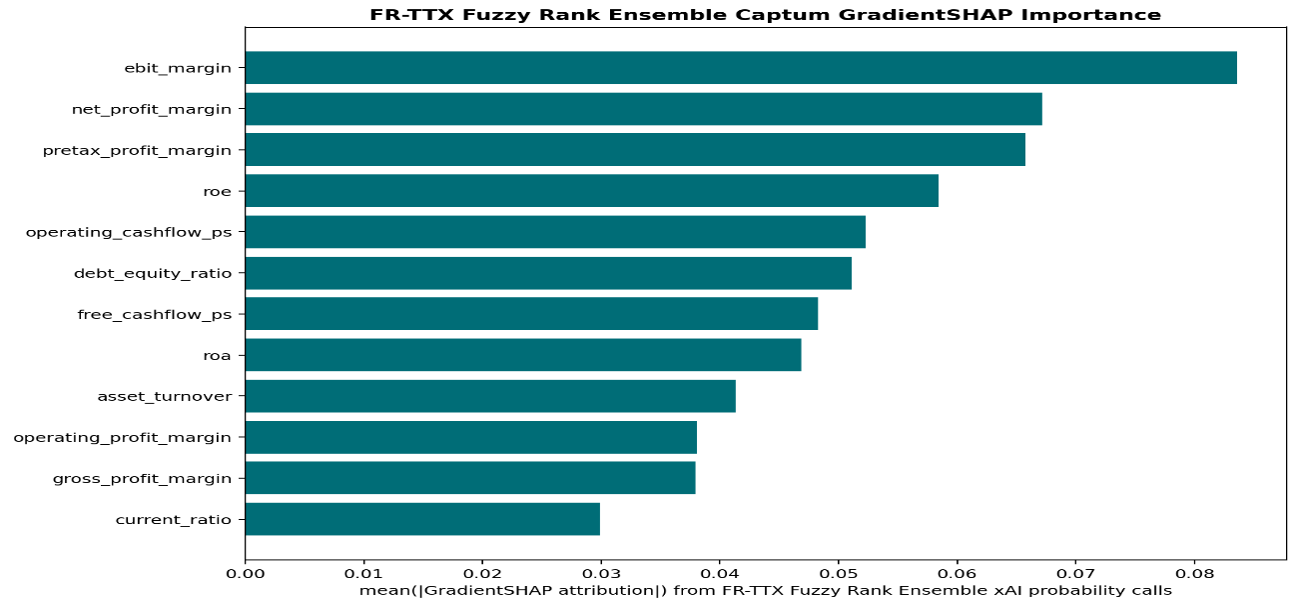
\includegraphics[width=0.55\linewidth]{acc-loss/shap-frttx.png} & 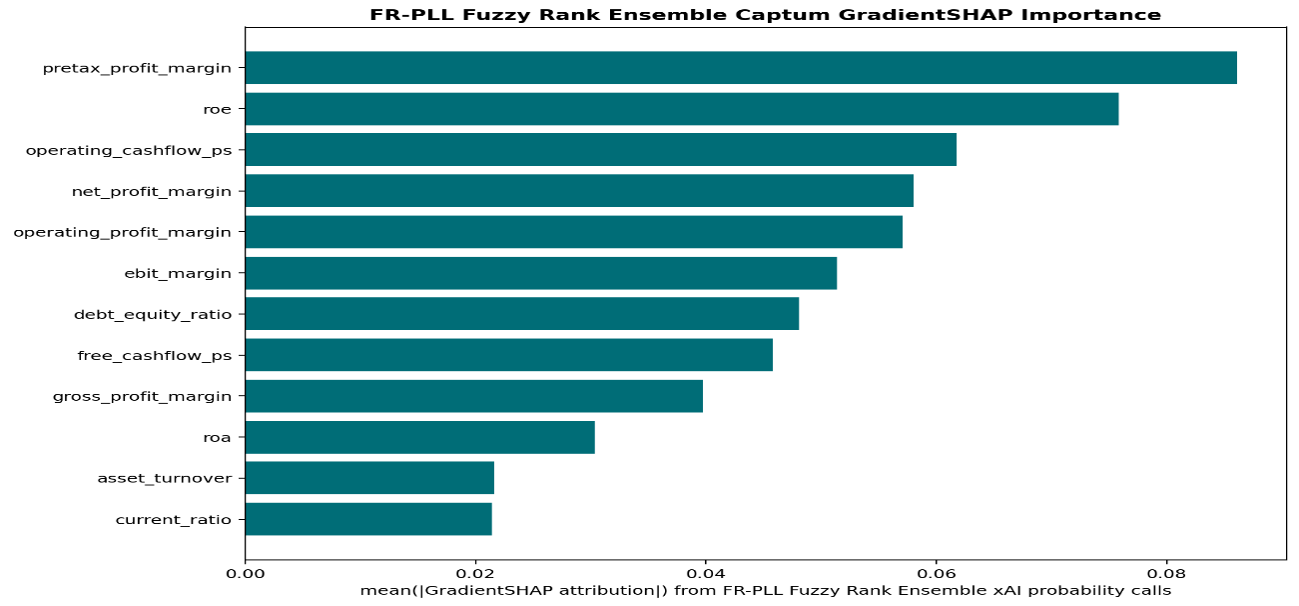
\includegraphics[width=0.55\linewidth]{acc-loss/shap-frpll.png} \\ \hline \textbf{Kết quả GradientSHAP của kịch bản 13} & \textbf{Kết quả GradientSHAP của kịch bản 14} \\ 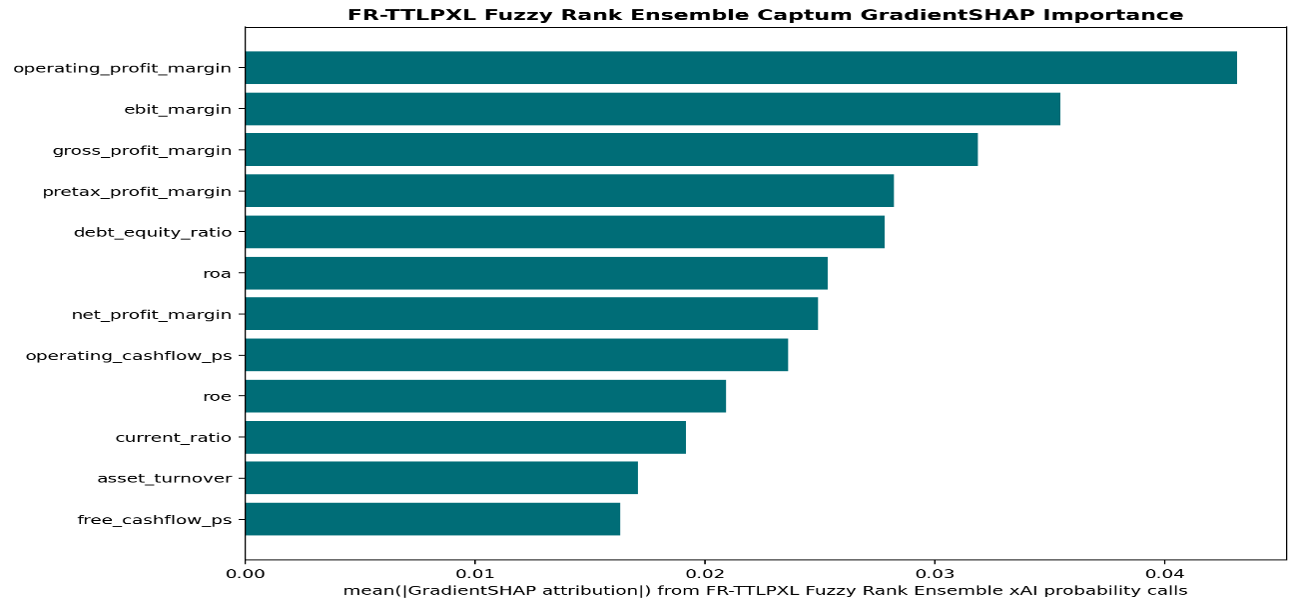
\includegraphics[width=0.55\linewidth]{acc-loss/shap-frttlpxl.png} & 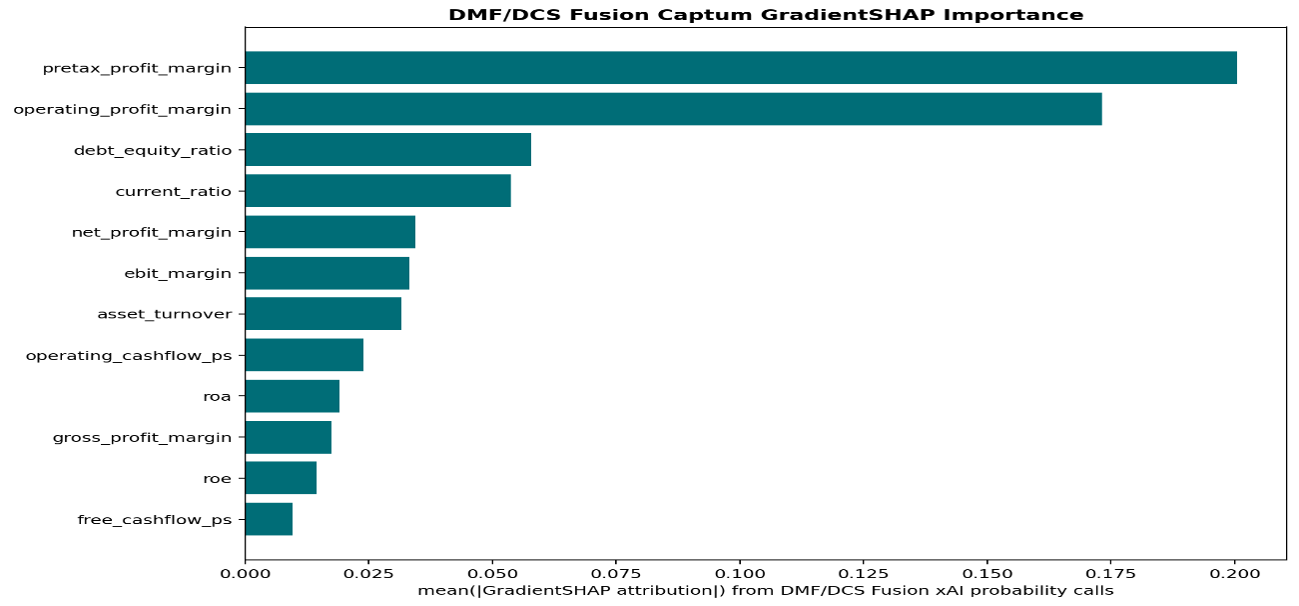
\includegraphics[width=0.55\linewidth]{acc-loss/shap-dmf.png} \\ \hline \end{tabular} \end{table}

GradientSHAP ghi nhận mức đóng góp lớn của các đặc trưng thuộc nhóm sinh lời, đòn bẩy và thanh khoản. Pretax Profit Margin và Operating Profit Margin thường xuất hiện trong nhóm đặc trưng có mức đóng góp cao. Debt-to-Equity Ratio và Current Ratio cũng được nhiều mô hình sử dụng khi phân biệt các nhóm rủi ro. T-LSTM và GraphSAGE còn phân bổ mức đóng góp cho ROA, ROE, Asset Turnover và các biến dòng tiền. Với DMF/DCS, các đặc trưng nổi bật gồm Pretax Profit Margin, Operating Profit Margin, Debt-to-Equity Ratio và Current Ratio. Các kết quả này nhất quán với vai trò thường được xem xét của khả năng sinh lời, đòn bẩy và thanh khoản trong phân tích tín dụng; chúng hỗ trợ diễn giải hành vi mô hình nhưng không xác lập quan hệ nhân quả.

\paragraph{LIME}
LIME được sử dụng như một phương pháp giải thích cục bộ, độc lập với mô hình. Trong nghiên cứu này, sau khi mô hình đưa ra kết quả xếp hạng tín dụng cho một doanh nghiệp cụ thể, LIME sẽ tạo ra nhiều mẫu dữ liệu nhiễu xung quanh mẫu gốc bằng cách thay đổi nhẹ các giá trị đặc trưng tài chính. Các mẫu nhiễu này sau đó được đưa vào mô hình đã huấn luyện để quan sát sự thay đổi trong xác suất dự báo. Trong biểu đồ LIME, màu cam thể hiện các đặc trưng có tác động làm tăng xác suất mô hình dự đoán vào lớp đang xét. Ngược lại, màu xanh thể hiện các đặc trưng có tác động làm giảm xác suất thuộc về lớp đó. Thanh càng dài thì mức độ ảnh hưởng của đặc trưng càng lớn.

\begin{table}[!htbp] 
\centering 
\caption{Kết quả LIME của các kịch bản trên tập kiểm thử} 
\label{tab:lime_results} 
\renewcommand{\arraystretch}{0.85} 
\setlength{\tabcolsep}{2pt} 
\begin{tabular}{|>{\centering\arraybackslash}m{0.47\textwidth}| >{\centering\arraybackslash}m{0.47\textwidth}|} 
\hline 
\textbf{Kết quả LIME của kịch bản 1} & 
\textbf{Kết quả LIME của kịch bản 2} \\ 
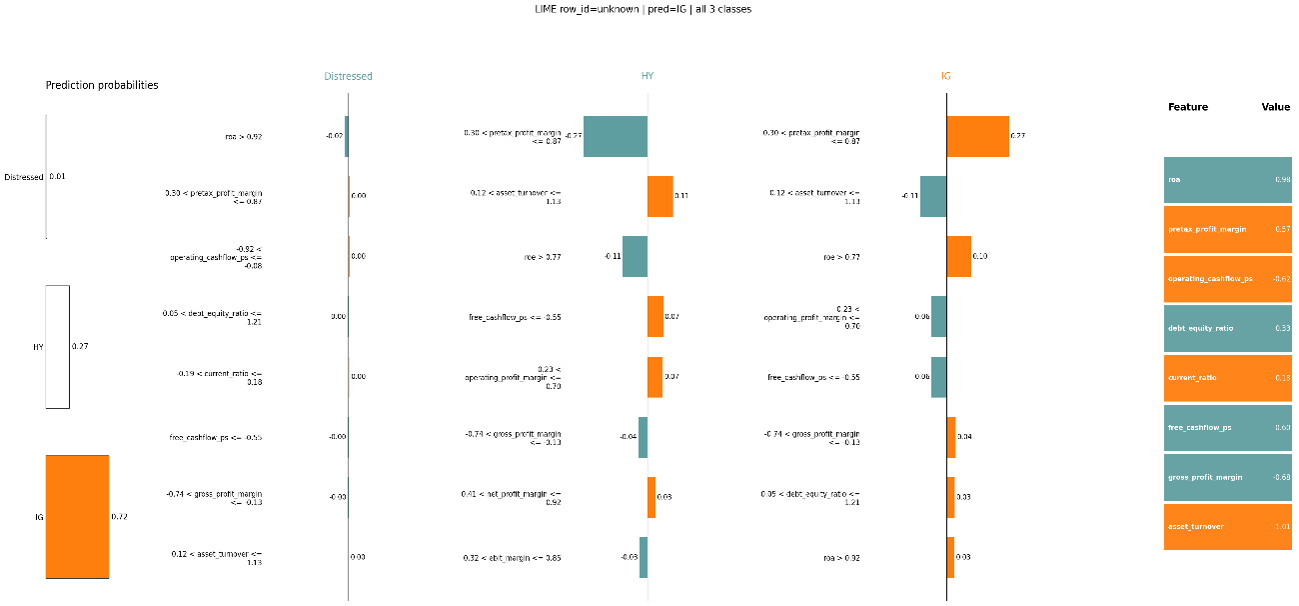
\includegraphics[width=0.55\linewidth]{acc-loss/lime-lightgbm.png} & 
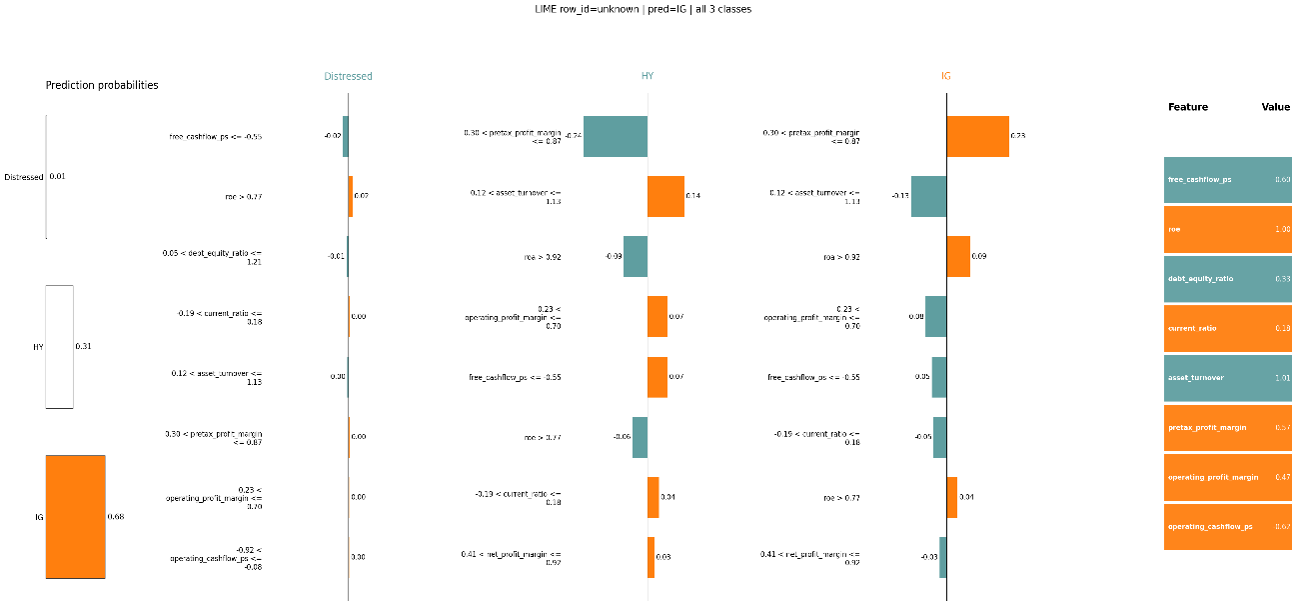
\includegraphics[width=0.55\linewidth]{acc-loss/lime-xgboost.png} \\ 
\hline 
\textbf{Kết quả LIME của kịch bản 3} & 
\textbf{Kết quả LIME của kịch bản 4} \\ 
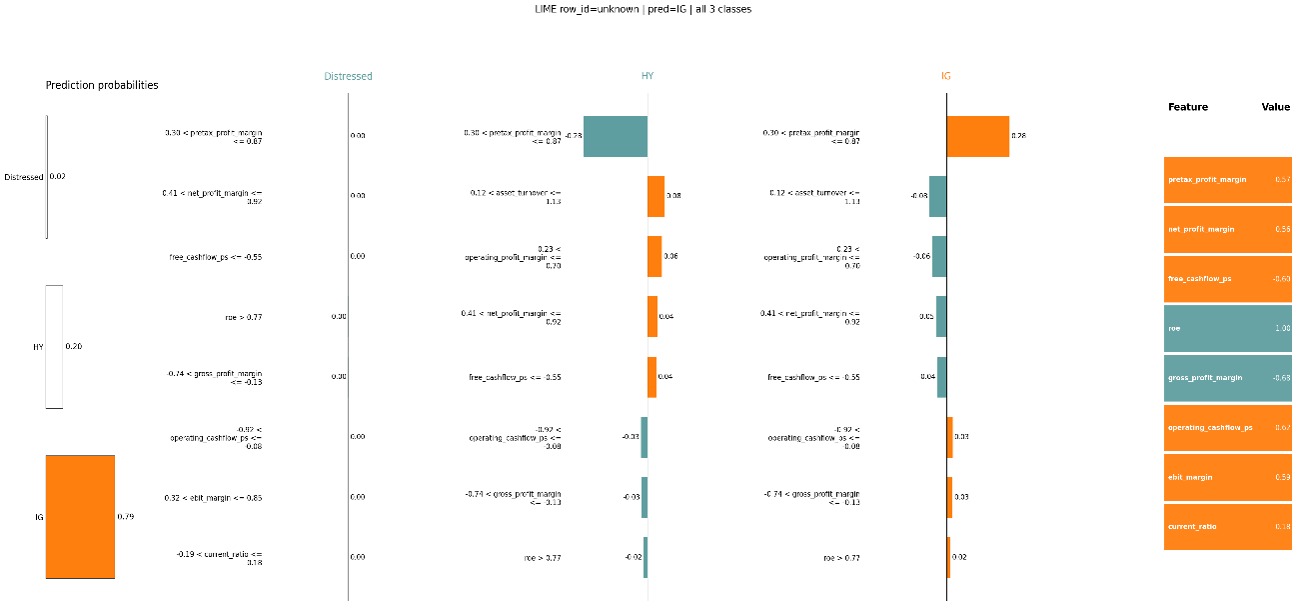
\includegraphics[width=0.55\linewidth]{acc-loss/lime-tcn.png} & 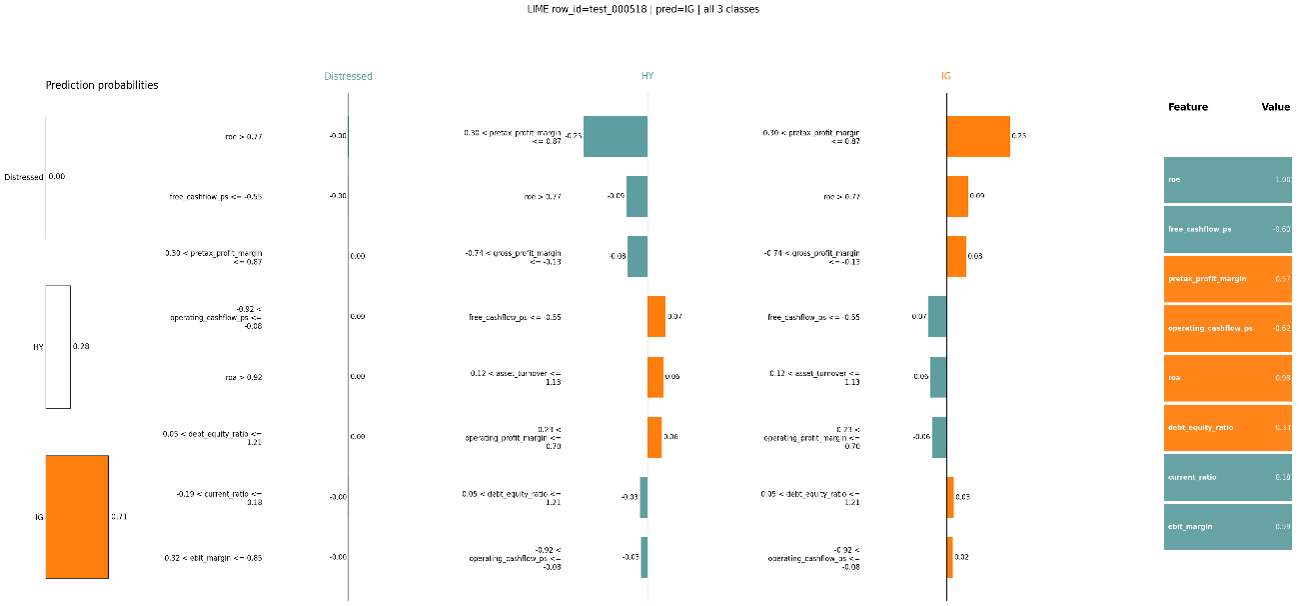
\includegraphics[width=0.55\linewidth]{acc-loss/lime-lstm.png} \\ 
\hline 
\textbf{Kết quả LIME của kịch bản 5} & 
\textbf{Kết quả LIME của kịch bản 6} \\ 
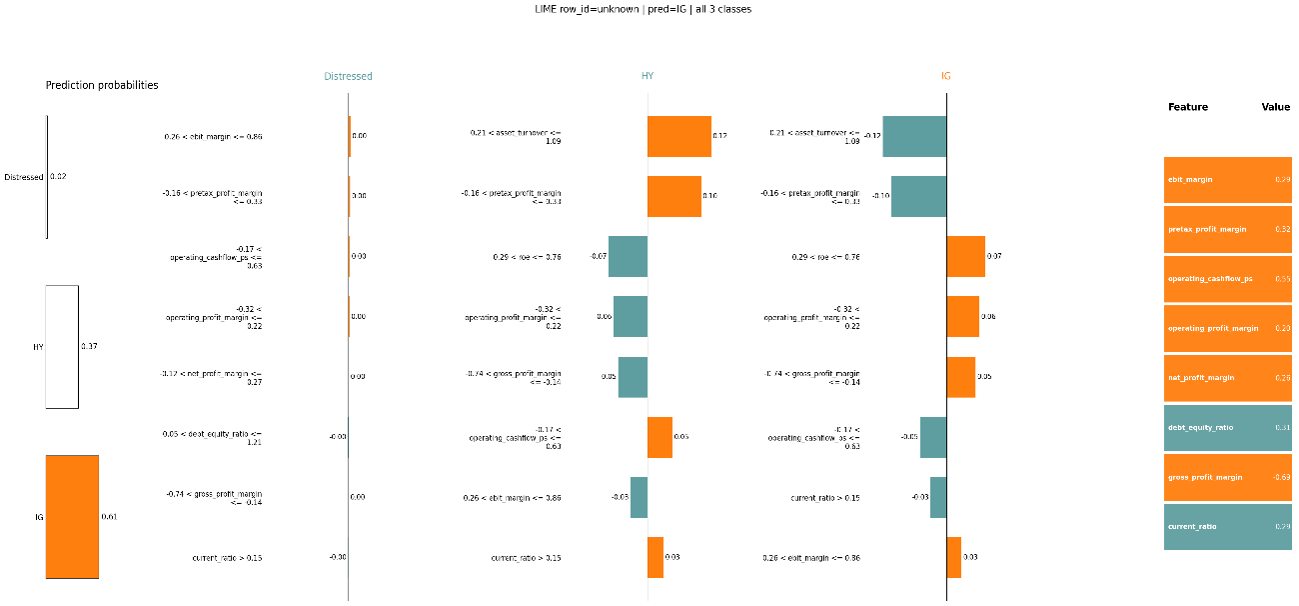
\includegraphics[width=0.55\linewidth]{acc-loss/lime-patchtst.png} & 
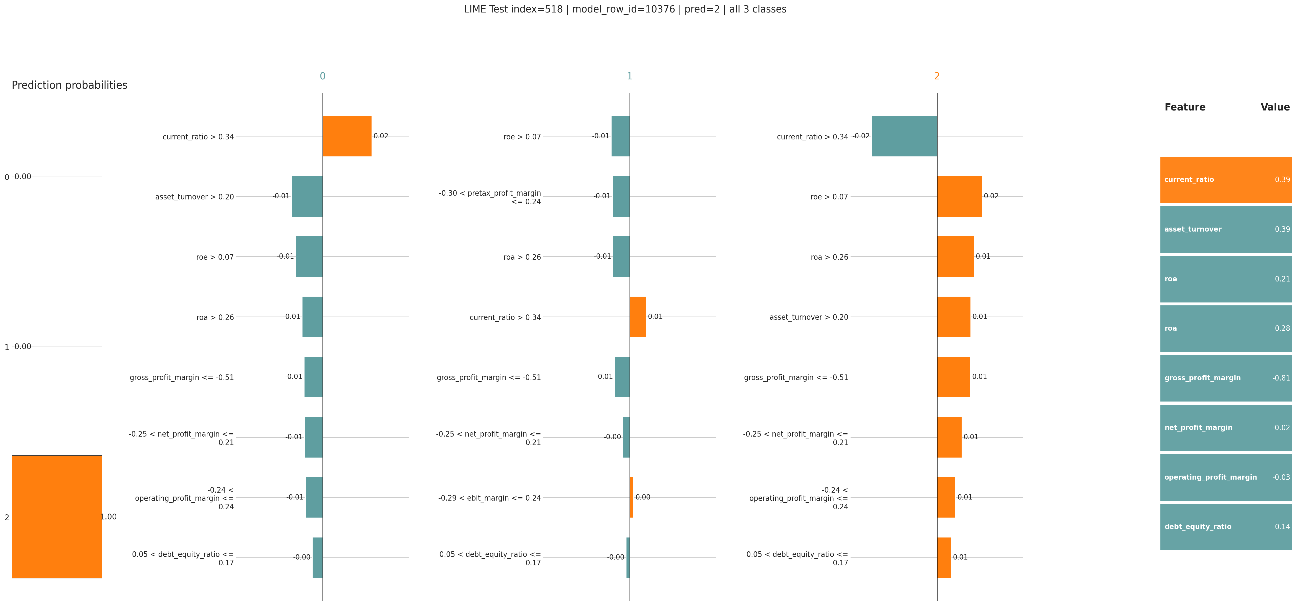
\includegraphics[width=0.55\linewidth]{acc-loss/lime-tlstm.png} \\ 
\hline 
\textbf{Kết quả LIME của kịch bản 7} & 
\textbf{Kết quả LIME của kịch bản 8} \\ 
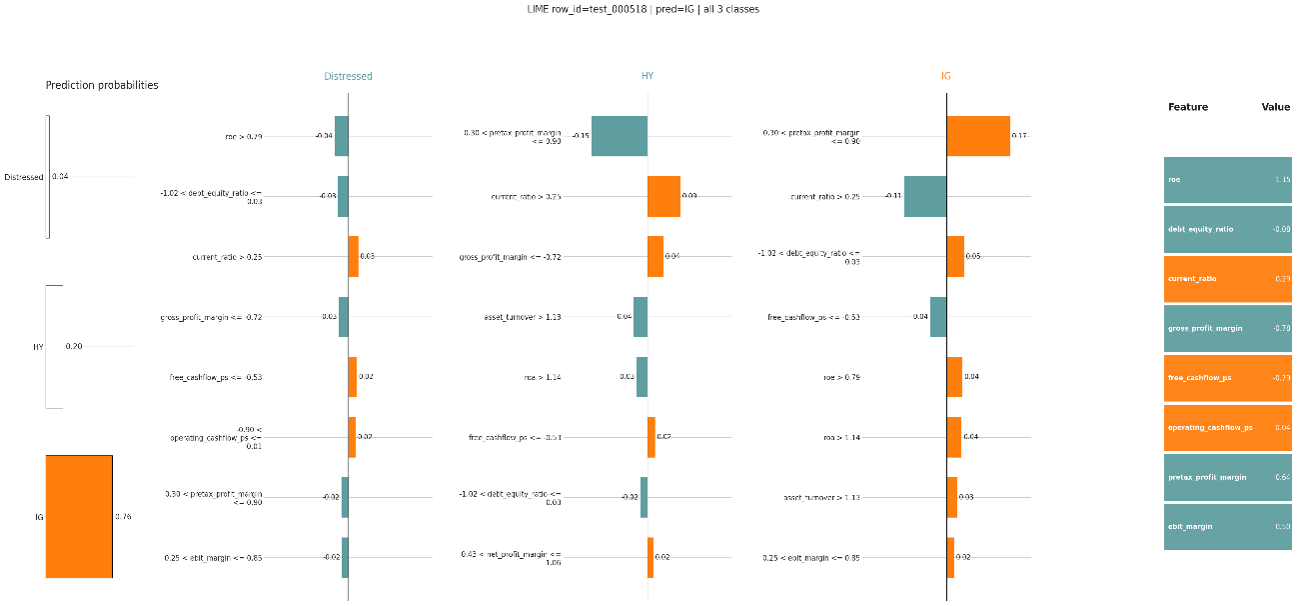
\includegraphics[width=0.55\linewidth]{acc-loss/lime-graph.png} & 
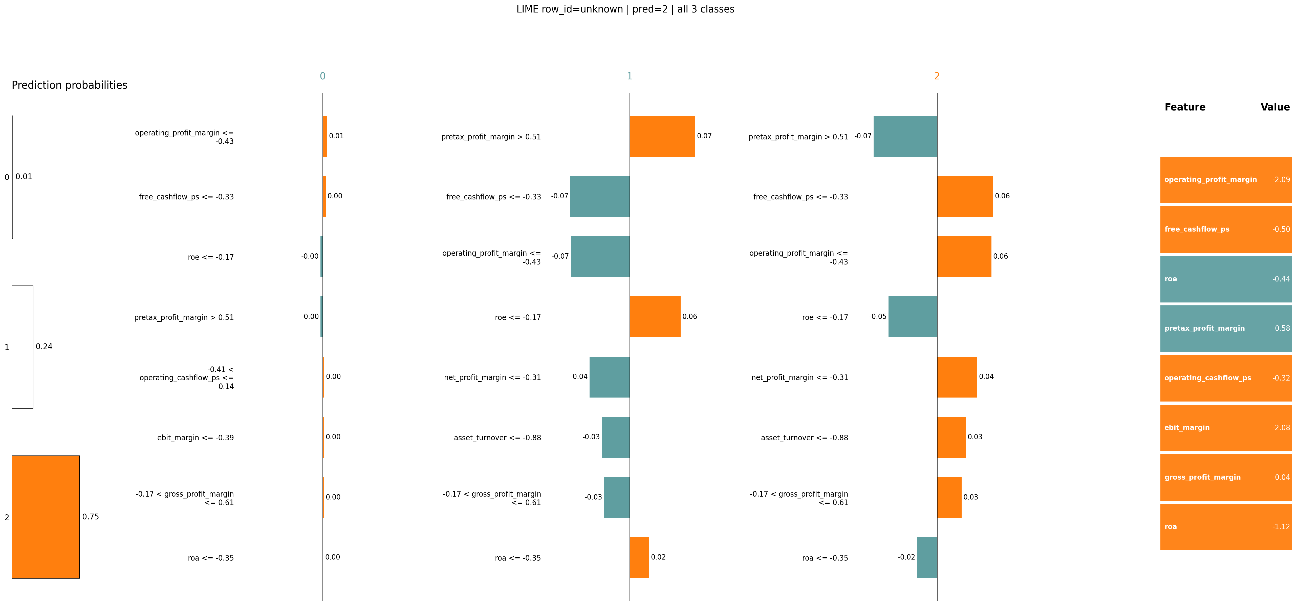
\includegraphics[width=0.55\linewidth]{acc-loss/lime-fittx.png} \\ 
\hline 
\textbf{Kết quả LIME của kịch bản 9} & 
\textbf{Kết quả LIME của kịch bản 10} \\ 
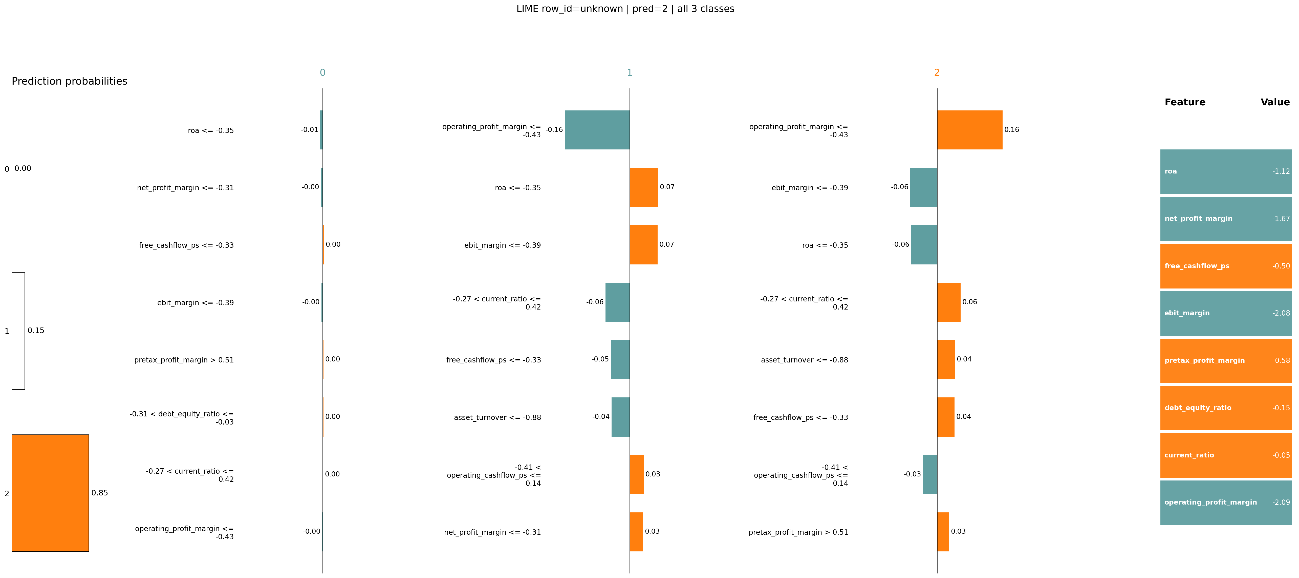
\includegraphics[width=0.55\linewidth]{acc-loss/lime-fipll.png} & 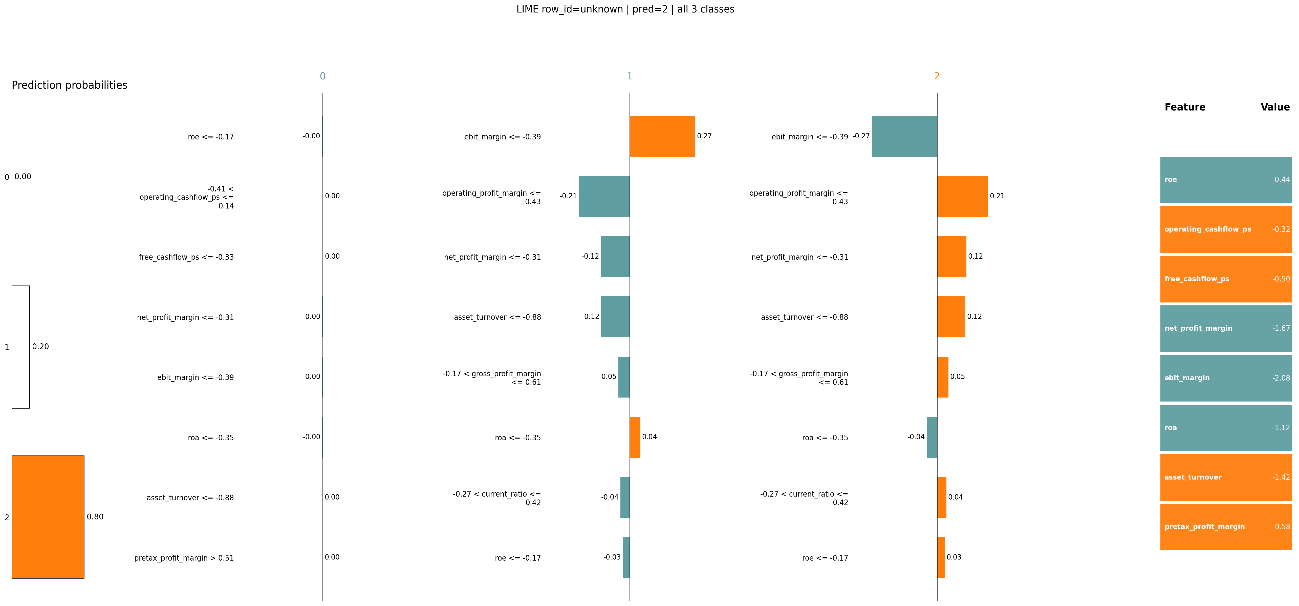
\includegraphics[width=0.55\linewidth]{acc-loss/lime-ttlpxl.png} \\ 
\hline 
\textbf{Kết quả LIME của kịch bản 11} & 
\textbf{Kết quả LIME của kịch bản 12} \\ 
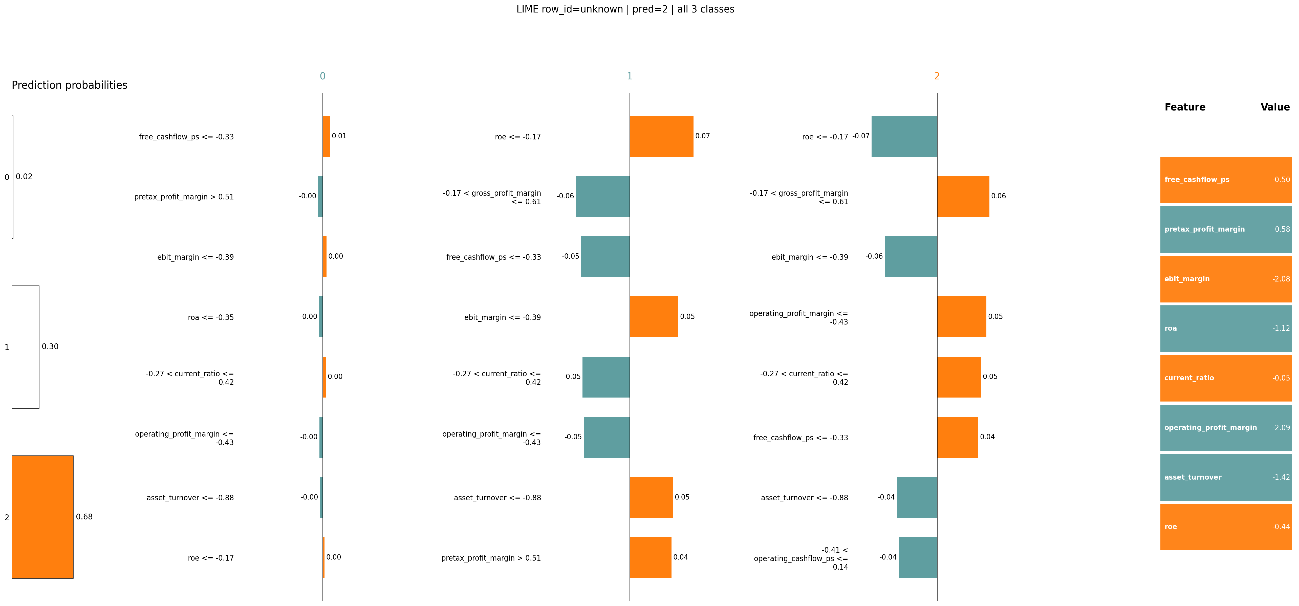
\includegraphics[width=0.55\linewidth]{acc-loss/lime-frttx.png} & 
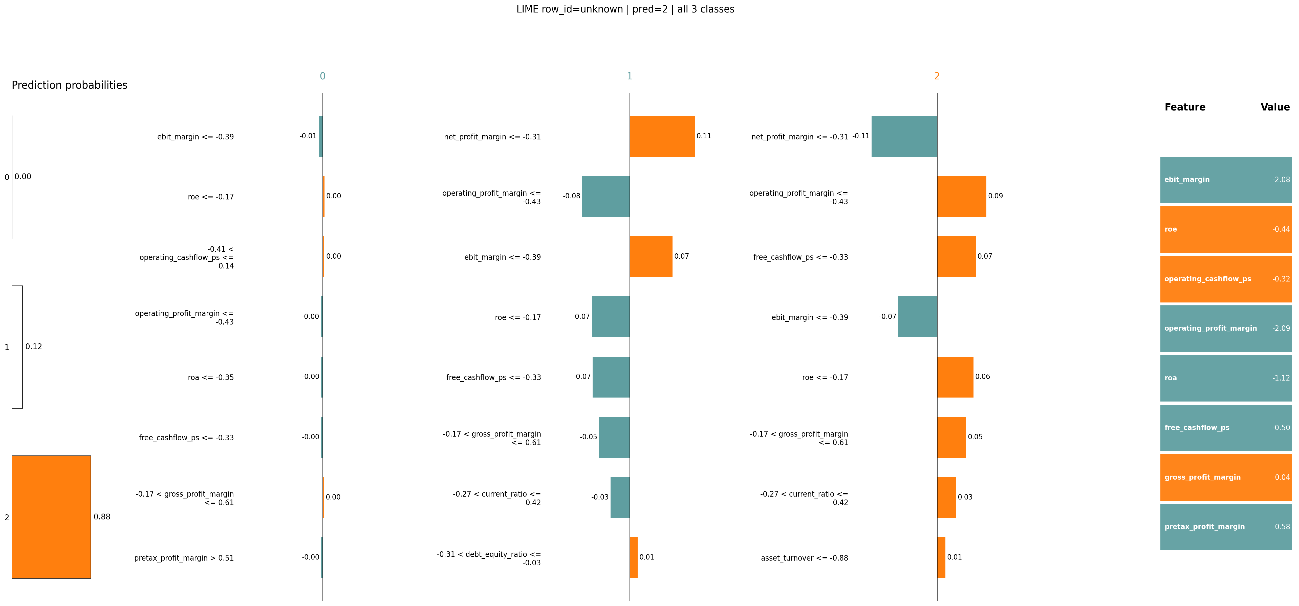
\includegraphics[width=0.55\linewidth]{acc-loss/lime-frpll.png} \\ 
\hline 
\textbf{Kết quả LIME của kịch bản 13} & 
\textbf{Kết quả LIME của kịch bản 14} \\ 
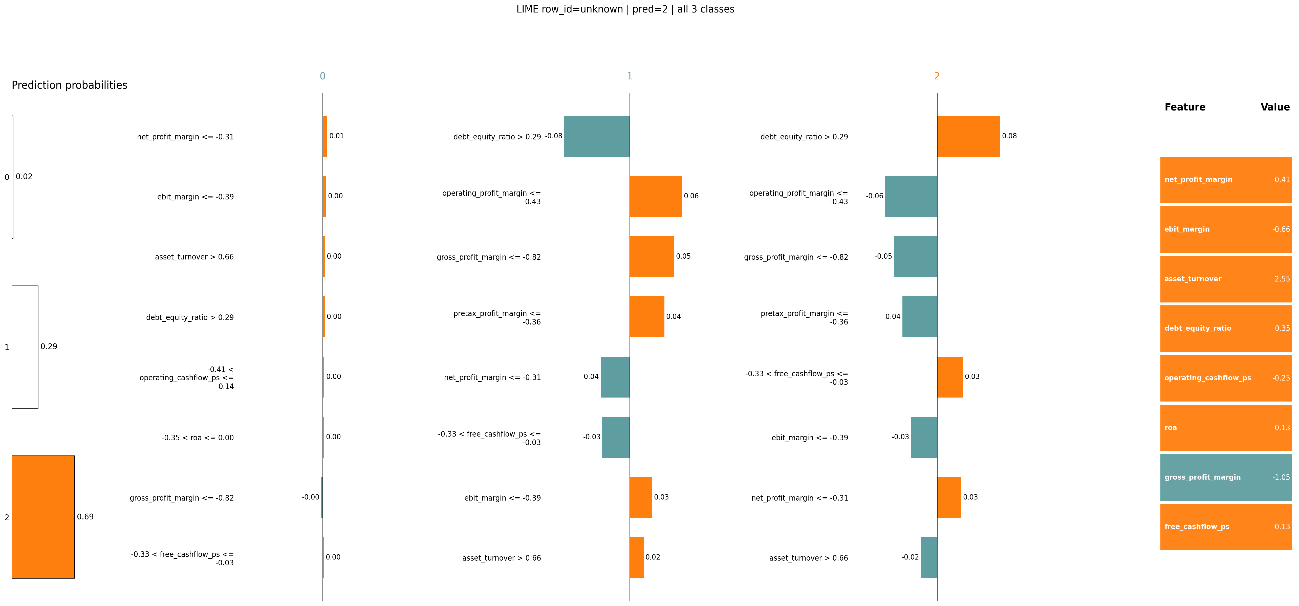
\includegraphics[width=0.55\linewidth]{acc-loss/lime-frttlpxl.png} & 
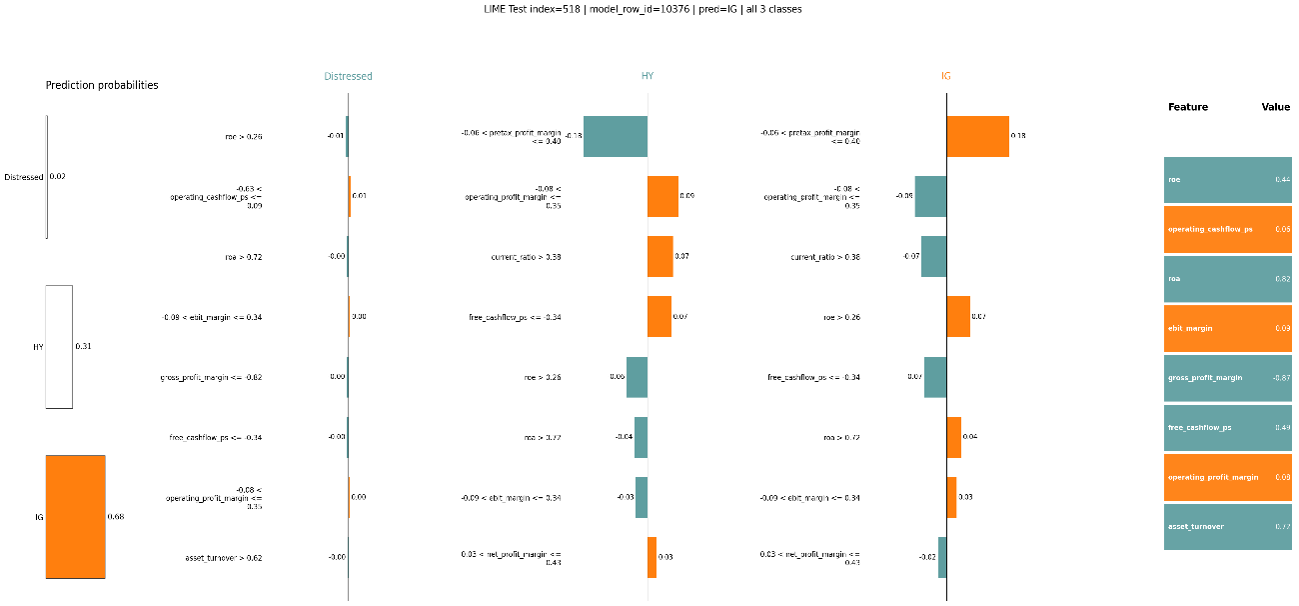
\includegraphics[width=0.55\linewidth]{acc-loss/lime-dmf.png} \\ 
\hline 
\end{tabular} 
\end{table}
GradientSHAP và LIME cung cấp hai mức diễn giải bổ sung. GradientSHAP mô tả mức đóng góp của đặc trưng trên nhiều quan sát, còn LIME xấp xỉ cục bộ hành vi của mô hình quanh một dự báo cụ thể. Hai phương pháp giúp truy vết các chỉ số tài chính liên quan đến dự báo, qua đó hỗ trợ tính minh bạch của hệ thống. Tuy nhiên, kết quả giải thích phụ thuộc vào mẫu nền, cách lấy mẫu nhiễu và cấu hình của từng phương pháp.
\subsection{So sánh và thảo luận}

\begin{table}[!htbp]
\centering
\caption{Bảng so sánh các kịch bản trên tập dữ liệu kiểm thử}
\label{tab:test_scenarios_comparison}
\begin{tabular}{c l c c c c}
\hline
\textbf{Kịch bản} & \textbf{Tên kịch bản} & \textbf{Accuracy (\%)} & \textbf{Precision (\%)} & \textbf{Recall (\%)} & \textbf{F1-score (\%)} \\
\hline
1  & LightGBM   & 91.99 & 91.88 & 91.99 & 91.90 \\
2  & XGBoost    & 92.05 & 91.94 & 92.05 & 91.95 \\
3  & TCN        & 91.93 & 91.76 & 91.93 & 91.78 \\
4  & LSTM       & 92.22 & 92.05 & 92.22 & 92.04 \\
5  & PatchTST   & 91.35 & 90.79 & 91.35 & 90.73 \\
6  & T-LSTM     & 92.51 & 92.10 & 92.51 & 92.23 \\
7  & GraphSAGE  & 92.34 & 92.35 & 92.34 & 92.34 \\
8  & FI-TTX     & 92.51 & 92.18 & 92.51 & 92.21 \\
9  & FI-PLL     & 92.34 & 92.20 & 92.34 & 92.22 \\
10 & FI-TTLPXL  & 92.16 & 91.75 & 92.16 & 91.82 \\
11 & FR-TTX     & 92.28 & 92.09 & 92.28 & 92.04 \\
12 & FR-PLL     & 92.40 & 92.26 & 92.40 & 92.27 \\
13 & FR-TTLPXL  & 92.46 & 92.33 & 92.46 & 92.31 \\
14 & DMF        & 92.98 & 92.67 & 92.98 & 92.60 \\
\hline
\end{tabular}
\end{table}
Bảng~\ref{tab:test_scenarios_comparison} cho thấy Accuracy dao động từ 91,35\% đến 92,98\%, còn F1-score dao động từ 90,73\% đến 92,60\%. Trong nhóm mô hình riêng lẻ, T-LSTM đạt Accuracy 92,51\% và F1-score 92,23\%; GraphSAGE đạt khoảng 92,34\% ở các chỉ số tổng thể. Trong nhóm học tập hợp mờ, FR-TTLPXL đạt Accuracy 92,46\% và F1-score 92,31\%. DMF đạt giá trị cao nhất ở cả bốn chỉ số tổng thể, nhưng mức tăng Accuracy so với T-LSTM và FI-TTX là 0,47 điểm phần trăm. Vì chưa thực hiện kiểm định thống kê hoặc đánh giá lặp lại trên nhiều lần chia dữ liệu, kết quả nên được diễn giải là bằng chứng thực nghiệm trên tập kiểm thử hiện tại, thay vì khẳng định ưu thế tổng quát.

\begin{table}[!htbp] \centering \caption{Kết quả so sánh giữa phương pháp đề xuất và các phương pháp khác} \label{tab:comparison_proposed_method} \small \renewcommand{\arraystretch}{1.35} \setlength{\tabcolsep}{4pt} \begin{tabular}{|p{3.2cm}|p{5.2cm}|p{3.0cm}|p{2.0cm}|} \hline \textbf{Nghiên cứu} & \textbf{Tập dữ liệu} & \textbf{Phương pháp đề xuất} & \textbf{Độ chính xác} \\ \hline Liu và Kok [63] & Bureau van Dijk (BVD) data platform & HTGNN & 70.57\% \\ \hline J. Darwish [64] & National Information and Credit Evaluation, Inc. (NICE) & Advanced feature selection & 72.03\% \\ \hline Morthens [11] & 318 doanh nghiệp huấn luyện và 112 doanh nghiệp chưa thấy trong huấn luyện & GRU; GRU-GCNGRU & 75.25\%; 74.44\% \\ \hline Mei Yang và cộng sự [65] & Compustat and Bloomberg & HDNN & 79.4\% \\ \hline Sanjiv Das và cộng sự [66] & Corporate Credit Rating và Synthetic Data & GNN+Tabular & 86.7\% \\ \hline D. T. T. Thùy và T. L. Hải [5] & 300 doanh nghiệp Việt Nam trong giai đoạn 2017--2019 & XGBoost & 87.73\% \\ \hline Fang và cộng sự [67] & Dữ liệu đa phương thức từ văn bản tài chính, chỉ số số và chuỗi thời gian & CNN-BiLSTM-AM & 88\% \\ \hline M. Kofune, K. Monden và S. Yamanaka [7] & AstraManager database, provided by Quick Inc & T-LSTM & 89.96\% \\ \hline B. Chen và S. Long [9] & People's Bank of China and Ji'an Rating & SMAGRU & 93.33\% \\ \hline Feng và cộng sự [66] & Bộ dữ liệu xếp hạng doanh nghiệp niêm yết tại Trung Quốc & CCR-GNN & 95\% \\ \hline \textbf{Phương pháp đề xuất} & Corporate Credit Rating with Financial Ratios và Corporate Credit Rating & \textbf{DMF} & \textbf{92.98\%} \\ \hline \end{tabular} \end{table}

Bảng~\ref{tab:comparison_proposed_method} tổng hợp các kết quả đã công bố với Accuracy từ 70,57\% đến 95\%. Tuy nhiên, các nghiên cứu sử dụng bộ dữ liệu, phân bố lớp, đặc trưng đầu vào và giao thức đánh giá khác nhau; vì vậy, các giá trị này không tạo thành một phép so sánh trực tiếp. Trên bộ dữ liệu của nghiên cứu hiện tại, DMF đạt Accuracy 92,98\%. Kết quả cho thấy cơ chế kết hợp T-LSTM và GraphSAGE là một hướng đáng khảo sát để khai thác đồng thời thông tin thời gian và cấu trúc đồ thị. Việc đánh giá khả năng tổng quát hóa cần thêm các bộ dữ liệu và giao thức thực nghiệm thống nhất.

\section{KẾT LUẬN}
Nghiên cứu xây dựng hệ thống xếp hạng tín dụng doanh nghiệp dựa trên các mô hình học máy, học sâu và mô hình đồ thị. Bảy mô hình riêng lẻ và bảy kịch bản học tập hợp được đánh giá trên ba nhóm IG, HY và Distressed. Trên tập kiểm thử hiện tại, DMF kết hợp T-LSTM và GraphSAGE đạt Accuracy cao nhất, ở mức 92,98\%. Mức chênh lệch so với các kịch bản gần nhất còn nhỏ và chưa được kiểm định thống kê, do đó kết quả chủ yếu gợi ý tiềm năng của cơ chế lựa chọn mô hình động.

GradientSHAP và LIME được sử dụng để hỗ trợ diễn giải dự báo. Pretax Profit Margin, Operating Profit Margin, Debt-to-Equity Ratio và Current Ratio thường có mức đóng góp đáng kể, nhất quán với vai trò của khả năng sinh lời, đòn bẩy và thanh khoản trong phân tích tín dụng. Tuy nhiên, Recall thấp của lớp Distressed cho thấy hệ thống vẫn hạn chế trong việc phát hiện doanh nghiệp có rủi ro cao. Các nghiên cứu tiếp theo cần đánh giá mô hình trên nhiều bộ dữ liệu, thực hiện kiểm định thống kê, cải thiện khả năng nhận diện lớp Distressed và bổ sung dữ liệu phi tài chính như tin tức, báo cáo thường niên, thông tin ngành và biến kinh tế vĩ mô.


\bibliographystyle{ieeetr}
\bibliography{thesis}

\end{document}
